introduction instructions
\chapter{Introduction}
This is a textual citation \citet{shannon44}. And this is a parenthetical citation \citep{shannon44}. You probably want to use the latter more often.

\section{Moving On}
Let's demonstrate a figure by looking at Fig.~\ref{bandwidth}. 

\begin{figure}[!h]
% Use "\centering" in floats (figure, table), but if you need to center
% some text (why?) use "\begin{center}...\end{center}".
\centering 
% Figure environments same as 0.8 * \textwidth please
% That does not necessarily mean the actual picture size,
% it is a guideline for the environment which could contain
% 2 or more pictures! Be consistent and follow the guidelines
% provided in your sources.
\includegraphics[width=0.8\textwidth]{images/bandwidth-colour.png}
\caption{Planning community bandwidth sharing costs. 
  Note caption capitalization.}
\label{bandwidth} 
% if you move the label it breaks the reference numbering; 
% always have it *after* the caption.
\end{figure}

% Remember how to include code with {\tt verbatim} 
% and to fix the tabs in {\sf python} in a verbatim environment? 
% It may be best to have an `include' command for code, 
% not to have to re-edit it all the time.
% \verbatimtabinput{code/mycode.py}



% Fix spacing before theorem environments
% \makeatletter\def\thm@space@setup{%
%   \thm@preskip=1.2\parskip\thm@postskip=0pt
%   }


% Reduce space before proof
% \renewenvironment{proof}[1][\proofname]{\par
%   \vspace{-\topsep}% remove the space after the theorem
%   \pushQED{\qed}%
%   \normalfont

  % For Arabic
% \usepackage{arabtex}
% \usepackage{utf8}
% \setcode{utf8}
% For tables:


% \usepackage{listings} % more flexible and complicated 
                        % than moreverb and algorithm
% 
% Others
% \usepackage[all]{xy}  %  if you use this uncomment \usepackage{etex} above to fix a conflict with tikz.
% \usepackage{sagetex}
% \usepackage{siunitx} % to typeset numbers, units, align decimals in tables.
% \usepackage{dcolumn} % less flexible but maybe faster than siunitx above.
% \usepackage{mathtools} % More maths, e.g. \mathclap.
%
% Others may be landscape, longtable, algorithm, algorithmic, etc.
% 
% ----------------------------------------------------------------------------
% An AIMS Essay can use the sectioning commands "\chapter", "\section",
% "\subsection". No "\subsubsection", "\paragraph", etc. They are disabled.
% 
% For Theorems and such, use the environments defined here:
% \begin{thm}...\end{thm} (or "lem", "defn", etc)
% 

% All other files are included via \input. 
% To compile in texmaker while viewing any of those
% without having to switch back, use
%   Options > Define Current Document as 'Master Document'
% To not have to close a PDF, remove viewpdf from quickbuild 
% and open the PDF (once) manually: it will auto-refresh or with control-r
% 
%-------------------------------------------------------------------------
% The abstract is the first thing we want to see. No acknowledgements or 
% dedications here. Fetch the abstract from a separate file.
% Please write it in English and in your mother tongue.
% An abstract should be less than half a page, so that both abstracts 
% (that is both languages) fit onto one page.
% We number roman numerals until the main body



% We switch to arabic numerals here where your page count starts
% Essays must be close to 30 pages long *starting here* and up to and including
% the conclcusion. It does not include the acknowledgements or references.
% 
% Figures may differ between topics, but they are not there
% to fill the pages -- they must add meaning.
% In general most figures should be 0.8 times the width of the page
% (perhaps wider in total when two or three columns of figures)
% See the example in chapter one for defining that. Be *consistent*
% in your presentation of information.

%-----------------------------------------------------------------------------
% Each chapter goes in a separate file
% Chapter titles are just examples
% Always have a question
% Note the Case Pattern used at AIMS


% \chapter{Introduction}

Over the last few years, advancements in large language models have primarily relied on scaling up the number of parameters alongside increasing dataset size and compute budgets. This strategy, often referred to as train-time compute scaling, has been remarkably effective, significantly and consistently improving model performance on tasks such as translation, general question answering, and sophisticated reasoning in mathematics and coding. However, the exponential growth in model size and the associated costs have become prohibitively expensive, pushing training budgets to the billion-dollar scale and raising concerns about resource sustainability, particularly as high-quality training data becomes scarcer.

Consequently, significant interest has shifted toward inference-time (or test-time) scaling techniques. Rather than focusing on costly retraining and larger models, inference-time scaling enhances existing models by dedicating additional computational resources during prediction. These methods enable models to "think longer" on challenging problems by dynamically generating multiple reasoning paths, employing voting mechanisms, or iteratively refining their outputs. Recent studies, such as DeepMind's compute-optimal scaling \citep{placeholder}, demonstrate how smaller models can achieve impressive performance through adaptive inference strategies, sometimes even outperforming substantially larger models.

In parallel with these developments, there has been a notable emergence of "reasoning" or "thinking" models, designed explicitly to enhance models' capabilities to reason through complex problems. A prime example is DeepSeek-R1, which explicitly trains models using reinforcement learning to produce long, structured chains of thought before providing an answer, enabling LLMs to systematically tackle tasks that were previously challenging even for large-scale models. DeepSeek released a series of small distilled models trained on reasoning datasets generated from the original R1 model, empowering them with remarkable reasoning capabilities and improving their performance relative to larger models.

Motivated by these developments, this work explores the promise of inference-time scaling techniques applied to small-scale language models-particularly those distilled from DeepSeek-that are specifically designed for coding and machine learning engineering tasks, areas still challenging even for frontier models. Smaller models have substantial advantages in accessibility, rapid deployment, and lower operational costs, but traditionally lack the advanced reasoning capabilities exhibited by larger models. Through systematic implementation and evaluation of strategies such as chain-of-thought prompting, iterative self-refinement, self-consistency, and other methods, this project aims to bridge the performance gap. Ultimately, this thesis evaluates the extent to which inference-time scaling can address complex tasks such as machine learning engineering. We demonstrate that, with carefully designed inference-time enhancements, small-scale models can significantly improve performance in complex coding and engineering contexts, presenting a viable and cost-effective alternative to training massive foundational models.

% \section{Introduction}
% The field of artificial intelligence is witnessing an unprecedented scaling race, where models with hundreds of billions of parameters demonstrate remarkable capabilities that seem to emerge from sheer computational scale. This phenomenon has created a stark divide in the AI landscape: while large proprietary models like GPT-4 and Claude achieve impressive performance on complex reasoning and coding tasks, smaller open-source alternatives lag significantly behind, creating substantial barriers to accessibility and democratization of AI capabilities.
% This performance gap is particularly pronounced in machine learning engineering tasks, where AI agents must not only write syntactically correct code but also reason about complex architectural decisions, debug intricate workflows, and navigate the nuanced requirements of end-to-end ML pipelines. Unlike general-purpose coding, ML engineering demands sophisticated reasoning about data preprocessing, model selection, hyperparameter optimization, and deployment considerations—capabilities that have remained largely the domain of expensive, proprietary models.
% The emergence of inference-time scaling (ITS) techniques offers a promising pathway to bridge this performance divide. Rather than requiring massive computational resources during training, ITS methods like chain-of-thought prompting, self-consistency, and iterative refinement allow smaller models to achieve enhanced performance by investing additional computation during inference. This paradigm shift suggests that the reasoning capabilities necessary for complex tasks might be accessible to open-source models through strategic application of ITS techniques.
% Recent advances in distilled reasoning models, particularly DeepSeek-R1's family of models ranging from 7B to 32B parameters, present an opportunity to test this hypothesis. These models demonstrate strong reasoning capabilities even at smaller scales, potentially providing the foundation needed for effective ML engineering agents when enhanced with appropriate ITS strategies.
% However, existing agentic frameworks have primarily focused on proprietary models accessed through APIs, leaving open-source implementations under-explored. While ITS techniques have been applied to coding tasks, their systematic integration with distilled reasoning models specifically for ML engineering remains largely uncharted territory. This gap represents both a technical opportunity and a practical necessity for organizations seeking to develop their own AI assistants without relying on expensive proprietary solutions.
% This thesis addresses these challenges by developing and evaluating an enhanced version of AIDE (AI-Driven Exploration), an open-source agentic scaffold specifically tailored for inference-time scaling with open-source models. Our approach integrates multiple ITS strategies—including self-consistency, iterative self-debugging, and modular task decomposition—with DeepSeek-R1 distilled models to create accessible ML engineering agents capable of autonomously tackling complex machine learning competitions.
% Contributions
% This work makes four key contributions to the field:

% High-Performance Open-Source Infrastructure: We develop a high-throughput parallel inference engine with multiprocess orchestration, enabling simultaneous experimentation across different models and tasks while maintaining competitive inference speeds for open-source deployments.
% Specialized Agentic Scaffold: We create an open-source agent framework specifically designed for the HuggingFace ecosystem, providing an alternative to proprietary API-based solutions and enabling broader accessibility to ML engineering automation.
% Systematic ITS Integration: We implement and evaluate multiple variants of AIDE, each incorporating different ITS strategies, providing a comprehensive exploration of inference-time scaling techniques for ML engineering tasks. These variants are made available as separate repository branches with a unified interface for strategy selection.
% Empirical Validation: We demonstrate that a 32B open-source model enhanced with appropriate ITS techniques can achieve performance comparable to GPT-4 Turbo on ML engineering tasks, reaching a practical level where the agent can autonomously solve Kaggle competitions end-to-end.

% Thesis Overview
% The remainder of this thesis is organized as follows. Chapter 2 provides essential background on agentic systems in research workflows, reviews the effectiveness of ITS techniques across domains, introduces the concept of agent scaffolding, and surveys existing benchmarks for evaluating ML engineering capabilities. Chapter 3 details our methodology, including the original AIDE framework, MLE-Bench evaluation protocols, and our systematic approach to integrating ITS strategies within the agentic scaffold. We discuss experimental design choices, cost considerations, baseline selection rationale, and provide detailed implementation insights for each ITS method. Chapter 4 presents comprehensive experimental results, including numerical evaluations of agent performance, analysis of observed behaviors, and discussion of failed approaches. Finally, Chapter 5 concludes with implications for future research and practical deployment considerations.
% Through this systematic investigation, we aim to demonstrate that the performance gap between proprietary and open-source models in ML engineering can be substantially reduced through careful application of inference-time scaling techniques, opening new avenues for accessible and democratized AI-driven automation in machine learning workflows. % Introduction is usually a chapter itself.
% \chapter{Background and Related Work}

\section{Background}

\subsection{Large Language Models (LLMs)}
Large Language Models (LLMs) are neural networks trained on extensive text datasets, capable of generating human-like text. Based primarily on the transformer architecture, these models utilize a straightforward predictive objective, leveraging enormous volumes of data to tackle complex problems and diverse natural language tasks [CITATION], including translation [CITATION], semantic analysis [CITATION], and information retrieval.

Recent advancements in LLMs, exemplified by models such as the GPT series [CITATION*3] and the Llama family [CITATION], have been driven by significant scale, reaching billions of parameters. This substantial scale has unlocked emergent abilities—advanced skills like reasoning and in-context learning—that smaller models typically do not exhibit. These emergent capabilities enable LLMs to solve arithmetic problems, answer intricate questions, and summarize complex passages, often without explicit task-specific training.

\subsection{Scaling Laws and Train-Time Compute}
Scaling lows shows how the performance of Large Language models improves in a predeictable way with the increase in the parameter size, training data and computationa; resources, openai ahs shown that LLMs performance as measured by metrics such as accuracy or perplexity follows a power low relationship with these scaling factors. Performance enhancements are steady yet exhibit diminishing returns as scale increases, motivating the development of increasingly larger models like PaLM and Chinchilla.

While scaling laws provided performance guarantees and drove a competitive race for building larger models, leading to current models in the hundreds of billions of parameters, practical limitations have surfaced. High-quality data is becoming scarce relative to growing model demands, and the significant costs and resource consumption associated with these models pose substantial challenges. Moreover, LLMs auto-regressive and token level prediction style is itself a limitation when it comes to complex reasoning tasks such as advanced mathematics or complex question answering. While recent years witnessed substantial developments in the models abilities, especially using post training and fine tuning, this requires massive computational resources and large scale datasets, encouraging researchers to to find cheaper approaches.

\subsection{Inference-Time Scaling (ITS)}
To address limitations associated with traditional scaling strategies, a new paradigm has emerged: inference-time scaling, also known as test-time scaling. Instead of allocating more resources to pretraining, this approach dynamically adjusts computational resources during inference, enabling models to "think longer" and thus handle more complex problems. Inference-time scaling involves techniques such as generating longer reasoning chains, sampling multiple possible answers, and iteratively refining outputs. This strategy has shown significant promise, allowing smaller models to surpass larger counterparts.

Techniques in inference-time scaling include:
\begin{itemize}
\item \textbf{Chain-of-Thought Prompting (CoT):} Encouraging models to explicitly generate intermediate reasoning steps.
\item \textbf{Iterative Self-Refinement:} Models iteratively identify and correct errors in their outputs.
\item \textbf{Self-Consistency:} Generating multiple independent outputs and selecting the most consistent result via voting.
\item \textbf{Verifier-Guided Search Techniques:} Utilizing reward-based verifiers or structured search methods to identify optimal answers from multiple generated solutions.
\end{itemize}

\subsection{Emergence of Reasoning Models}
Recent developments have highlighted the emergence of models focused on reasoninging specifically designed to enhanthe capabilities in multistep  logical and mathematical reasoning. These reasoning models utilize inference-time strategies like structured prompting, external tool usage, and systematic search without altering model weights. Techniques such as ReAct, PAL, Toolformer, and Tree-of-Thoughts have demonstrated significant improvements in reasoning abilities.

DeepSeek-R1 serves as a notable landmark, explicitly trained via reinforcement learning on structured reasoning datasets to generate coherent reasoning chains, significantly improving performance on complex reasoning tasks. DeepSeek's release of smaller distilled models, trained on datasets generated by R1, demonstrates the potential of distillation combined with structured inference strategies, achieving performance comparable or superior to larger models.

* the effect of rl training on producing long chains of thoughts
* the distilled models that were trained on the reasoning datata from R1 model

\subsection{Agentic Systems and Scaffolding}
"Scaffolding" reffers to code built up around an LLM in order to augment its capabilities. This does not typically include code which alters the LLM's internals, such as fine-tuning or activation steering. People use scaffolding because it can allow LLMs to use tools, reduce error rates, search for info, all of which make LLMs more capable.
Common types of scaffolds include:
Prompt templates: Perhaps the simplest scaffolds, "prompt templates" are just prompts with some blank sections to be filled in at runtime using some local data. E.g., a template like "You are a good assistant. The date is {INSERT DATE HERE}. Tell me how many days are left in the month." can be filled in with the current date before being used to prompt an LLM.
Retrieval Augmented Generation (RAG): For tasks which have some associated data, RAG is a way of automatically adding task-relevant info to prompts. RAG does this by looking for snippets of text/data in the database which are relevant to the user's prompt, and then adding those snippets to the prompt.
Search engines: Similar to RAG, giving an LLM access to a search engine lets it find info relevant to its prompt. Unlike RAG, the LLM decides what to search for and when.
Agent scaffolds: Scaffolds which try to make LLMs into goal-directed agents, i.e., giving an LLM some goal/task to perform, and ways to observe and act on the world. Usually, the LLM is put into a loop with a history of its observations and actions, until its task is done. Some agent frameworks give LLMs access to much more powerful high-level actions, which saves the AI from repeating many simple primitive actions and, therefore, speeds up planning.

Agent scaffolds are characterized by their capacity for perception, planning, and action within an environment, often governed by an iterative process that refines, reflects, and improves the solution over multiple cycles.

While agents scaffolds can be used in different domains and wide array of tasks, there has been increasing interest dedicated to developing agents capable of automating the machine learning research and engineering process. A notable example is the [AI scientist] system, which presents an end-to-end pipeline designed to automate the research workflow. Currently, data science, machine learning engineering, and more generally, coding agents and assistants have shown consistent improvements. as we now see agents like Gihub Capilot, Cognition | Introducing Devin, Cursor, or Claude code exhibit phenomenon coding abilities, but there is no significant progress in their open-source coding agents. 

The nature of coding problems presents a unique challenge for LLMs compared to other reasoning tasks, such as mathematics. In mathematical reasoning, there is often a single, unambiguously verifiable answer that can be derived through logical deduction. Conversely, generating a coding solution involves not only producing syntactically correct and executable code, but also navigating a vast solution space, where multiple functionally equivalent but structurally diverse implementations can exist. Crucially, the correctness and optimality of a coding solution often necessitate empirical validation through actual code execution and looking at traceback, rather than purely symbolic or logical verification. This inherent complexity, which demands iterative refinement and empirical testing, underscores the critical need for sophisticated agentic systems that can autonomously generate, execute, and iteratively refine solutions, even for highly capable foundational models.

\subsection{Relevance and Challenges in Coding and ML Engineering Tasks}
Machine learning engineering and coding tasks represent particularly challenging yet highly relevant applications for inference-time scaling due to their inherent complexity and precision requirements. Benchmarks like HumanEval, MBPP, and MLE-Bench exemplify these tasks, providing challenging evaluation contexts.

However, significant gaps persist in current research, such as limited open-source implementations and insufficient evaluation on realistic, complex coding tasks. This project explicitly addresses these gaps by systematically applying inference-time scaling techniques to small-scale distilled reasoning models, aiming to substantially enhance their performance and practical applicability in coding and ML engineering domains.

CITATION NEEDED
\section{Related Work}
% * systems such as aide, or any open source implemntaion
% * infercne time and how it improves small models
% *** I should find example for MATH of course ***
 

% \subsection{Inference-Time Scaling Techniques in the Coding Domain}

% The core idea in Inference-Time Scaling (ITS) for code generation is to allow a model to generate and evaluate multiple solutions or reasoning steps before finalizing an answer, much like a programmer iteratively writes, tests, and debugs code. This can enable smaller models to achieve results on par with much larger models by compensating with clever search and reasoning. Below is an overview of relevant ITS
% strategies in the context of code generation:

% \subsection{Multiple Sampling and Majority Voting}:
% The simplest form of test-time compute scaling is to sample many outputs and pick the best, much like an ensemble methods, this can be very effective as the LLMs output are not generally deterministic, and in theory. For coding, this might mean prompting a 7B model 10 times for a function implementation and then using a heuristic to choose among those attempts. Majority voting is one approach where if multiple samples converge on the same answer, that answer is taken as more likely correct. However, for complex coding problems (especially ones without a single "exact" answer), majority voting may not help much – if the model tends to make a consistent mistake, all samples will be wrong in the same way. Nonetheless, for simpler tasks (like leetcode-style problems with fixed outputs), self-consistency via voting can reduce random errors. 

% A more effective variant is "Best-of-N" selection, where instead of voting, the best candidate out of N is chosen based on an evaluation function. In coding, the evaluation function could be a set of unit tests or a code quality metric. For example, generate 5 different code solutions and then run all of them against some test cases, picking the one that passes the most tests. 

% This Best-of-N strategy was found to significantly improve math problem solving for small
% models when using an automated judge, and for code it can similarly boost correctness if a reliable evaluator is available. In practice, Best-of-N requires more inference runs (linear in N) and possibly running a reward model or tests to rank outputs, but it's a straightforward way to leverage extra compute. 

% Iterative Self-Improvement (Self-Reflection and Debugging): instead of generating
% many answers independently, another approach is to have the model improve
% a single solution by self-correcting mistakes in an iterative way. Techniques like self-
% reflection, as well as Self-Debugging and Reflexion feedback loops.

% The general pattern is: the model produces an initial solution, then the model (or another instance of it or another role controlled by the system prompt) is asked to inspect that solution for errors or flaws, and propose a fix, and this process repeats. In code generation, this mirrors the edit-compile-fix cycle programmers use. For example, Chen et al. (2023) introduced Self-Debugging, where an LLM is taught via examples to run the code (or at least simulate running it) and then asked to explain what the code is doing and identify any mistakes based on either runtime results or logical reasoning. Notably, their approach has the model look at execution results (e.g. error messages or failed tests) without human feedback, and then pinpoint the bug and fix it – effectively the model learns to debug itself. This yielded state-of-the-art results on several coding tasks, improving accuracy by up to 12\% on test-driven benchmarks by iteratively correcting errors.

% Reflexion, a recent idea for general reasoning, has the model generate a brief "reflec-
% tion" after a failed attempt, explaining what went wrong and how to adjust its next attempt. This reflection is then prepended to the next query so the model won't repeat the mistake. In coding, a similar approach can be used: after an unsuccessful run (say the model's code didn't produce a valid output or scored poorly), the agent can prompt the model to reflect: "Why did your solution perform poorly? What could be improved?" and use that answer to guide the next code revision.

% These self-corrective loops leverage the model's reasoning ability at inference time to gradually approach a correct solution, instead of having a perfect answer in one shot. 

% They are modular (generator + debugger) and don't require training new models – only cleverly designed prompt sequences and possibly a memory of past failures. This family of techniques is arguably one of the most promising for coding, because coding tasks naturally provide feedback (errors, test outcomes)
% that the model can learn from on the fly. 

% Search-Based Approaches (Beam Search, Tree-of-Thought, MCTS): Classic AI search algo-
% rithms can be applied at inference to guide the generation of code. Instead of treating the LLM as a black box that generates one solution, we can treat partial generations as states in a search tree. For instance, beam search is a technique where at each step of code generation, multiple possibilities are kept (`the beam') and the search explores several paths, not just the single most likely token sequence. In natural language generation this is tricky (due to the immense branching), but for structured tasks like code, researchers have attempted to incorporate it. A recent Hugging Face case study used beam search guided by a learned reward model to have a 1B model solve math problems step-by-step, expanding only the promising reasoning paths. 

% They further introduced Diverse Verifier Tree Search (DVTS), which explicitly encourages exploring diverse branches and uses a verifier to prune incorrect logic, preventing the search from converging on a wrong answer too early. Translating this to code: one could imagine generating different code approaches, one branch tries a neural network, another branch tries a gradient boosting model) and then evaluating both, continuing to refine whichever looks more promising. A search algorithm (DFS or BFS with pruning) explores combinations of these thoughts to find an overall successful solution. In coding tasks, a "thought" could be a high-level plan or a code snippet. By evaluating partial solutions (e.g., does the code run up to a certain point without error? Does a partial result look plausible?), an agent can systematically search for correct code. An Example is the S*framework augments parallel sampling with sequential debugging – generating multiple initial programs, then iteratively debugging each using execution feedback, and then selecting the best program at the end. It even uses adaptive test generation during selection: the LLM is asked to come up with specific inputs that differentiate two candidate programs, then it runs both programs on those inputs to see which one fails. Such adaptive search is quite advanced – effectively using the model to adversarially test its own outputs – and it was shown to let a 3B coder outperform models as large as 70B on code benchmarks. 

% In summary, search-based ITS techniques treat code generation as a search problem, leveraging multiple candidates and systematic exploration. These methods require more
% complex control logic (to manage the search and comparisons) and sometimes an external judge (which can be the model itself in a verifier role), but they can dramatically improve coverage of the solution space for tricky coding tasks.

% Tool-Assisted and Modular Reasoning: Another angle for inference-time improvement is
% giving the model external tools or modules to use while solving the problem. In coding, the
% most pertinent tool is a Python interpreter or execution environment. An agent with tool use ReAct paradigm or API toolformer approaches can decide to run a piece of code to see
% what happens and incorporate the result into its next step. For example, if the task is to write a function, the agent could generate a candidate, execute it on some test inputs, and observe the outputs or any exceptions, then adjust accordingly. for general coding tasks, letting the model search error messages or look up API usage could help a smaller model correct mistakes that it wouldn't know how to fix from training data alone. 

% A modular approach could also mean splitting the problem among specialized modules: for instance, a static analyzer module could lint the model's code for syntax errors or bad practices, and a test generator module could produce unit tests for the code. These modules might themselves be LLM prompts
% or traditional programs. Their feedback can then be fed into the model's next inference. Because
% these happen at inference time (no weights changed, just additional computation/feedback), they
% fall under ITS. example for this is to integrate a type-checker: the model writes Python code, run a type checker or even a lightweight symbolic execution to catch obvious misuses, then prompt
% the model with "The following variables might be undefined." By incorporating such tools in the loop,
% we can elevate a smaller model's performance – it doesn't need to have all knowledge internally
% if it can query an external helper. The ReAct framework demonstrated that even a single LLM
% agent can use tools effectively by interleaving reasoning and acting steps. In coding, this could
% mean the agent alternates between "think about how to solve" and "try running this piece" actions.
% Overall, tool-assisted inference allows modularizing the task and providing grounded feedback

% Agentic Scaffolding and Role Decomposition: Closely related to the above, many agent
% frameworks split the problem-solving into multiple roles or phases. An example would be a planner-executor paradigm: first prompt the LLM to write a high-level plan or pseudo-code, then in a second prompt have it implement that plan in actual code. This helps because the model can focus on logical planning in one stage and syntax in another, reducing cognitive load. Another example is having a separate critic agent: one model (or one chain of prompts) produces a solution, and another model (or later prompts of the same model) evaluates that solution. For coding, one might have: a "data scientist" agent that decides what model to use, a "coder" agent that writes the code, and a "tester" agent that runs and verifies the code. All could be orchestrated in one loop. Such modular, agentic strategies can dramatically improve outcomes since mistakes caught by one module can be fixed before the final answer. They don't require additional training if we use the same base model with different prompts, though they
% incur more inference calls. This approach has been demonstrated in other domains (for example, decomposition into sub-agents for math word problems). 
% In code generation, the AutoKaggle system (2024) uses a multi-agent workflow with different specialists collaborating on a competition problem. While complex, this shows promise in handling the many facets of ML engineering (data cleaning, modeling, hyperparameter tuning) through coordinated inference-time work.
% In summary, inference-time scaling in coding tasks includes sampling-based methods (generate many solutions, then filter or vote), iterative improvement (let the model refine its answer using feedback,
% either self-generated or from executing code).

% \subsection{Machine Learning Engineering Benchmarks and Automated research workflow}

% coding benchmarks like swebench*
% agent scaffolds like AutoML (H2O) etc *
% AI scientist, and kaggle agents.*


% Background and Related Work
% This chapter provides the technical foundation necessary to understand our approach to enhancing open-source machine learning engineering agents through inference-time scaling. We begin by establishing key concepts in large language models and their inference mechanisms, then explore how inference-time scaling has proven effective across various domains, before examining the specific challenges and opportunities in ML engineering automation.
% 2.1 Large Language Models and Inference
% 2.1.1 Foundation Models and Training Paradigms
% Large Language Models (LLMs) are transformer-based neural networks trained on vast text corpora to predict the next token in a sequence. The training process typically involves three stages: pretraining on diverse internet text to learn general language understanding, supervised fine-tuning on curated instruction-following datasets to align with human preferences, and reinforcement learning from human feedback (RLHF) to further refine behavior through preference optimization techniques like PPO or DPO.
% The pretraining phase establishes the model's foundational capabilities—its understanding of syntax, semantics, factual knowledge, and reasoning patterns. Fine-tuning then shapes how these capabilities are expressed, teaching the model to follow instructions, engage in dialogue, and perform specific tasks. This multi-stage approach has proven crucial for creating models that are both knowledgeable and helpful.
% 2.1.2 Inference Mechanisms and Decoding Strategies
% During inference, LLMs generate text through autoregressive decoding, where each token is predicted based on all previous tokens in the sequence. The decoding process involves several key parameters that significantly influence output quality and diversity:
% Temperature controls the randomness of token selection, with lower values (0.1-0.3) producing more deterministic outputs and higher values (0.7-1.0) increasing creativity and variability. Top-k sampling restricts token selection to the k most probable candidates, while top-p (nucleus) sampling dynamically adjusts the candidate pool based on cumulative probability mass, typically set between 0.8-0.95 for optimal balance between coherence and diversity.
% Beam search represents an alternative decoding strategy that maintains multiple candidate sequences simultaneously, exploring different paths through the probability space. While computationally more expensive than sampling methods, beam search can produce higher-quality outputs for tasks requiring careful reasoning or structured responses.
% The choice of decoding strategy and parameters can dramatically affect model performance on complex tasks, making inference-time optimization a critical consideration for practical applications.
% 2.1.3 Inference Engines and Deployment
% Modern LLM deployment relies on specialized inference engines that optimize memory usage, computational efficiency, and throughput. Popular frameworks include vLLM, which uses PagedAttention for efficient memory management, TensorRT-LLM for NVIDIA GPU optimization, llama.cpp for CPU inference, and Text Generation Inference (TGI) for production deployments.
% These engines implement various optimization techniques including dynamic batching, continuous batching, and KV-cache management to maximize hardware utilization. The choice of inference engine can significantly impact both the speed and cost of serving LLMs, particularly important considerations when deploying open-source models at scale.
% 2.2 Inference-Time Scaling: Beyond Training Scale
% While the field has long focused on scaling models through increased parameters and training compute, inference-time scaling (ITS) offers an alternative paradigm where additional computation during inference enhances model capabilities without requiring larger models or extended training.
% 2.2.1 Core ITS Techniques
% Chain-of-Thought (CoT) Prompting emerged as one of the first successful ITS techniques, where models are prompted to "think step by step" and show their reasoning process explicitly. This simple modification has shown remarkable effectiveness across mathematical reasoning, logical puzzles, and complex problem-solving tasks, often improving performance by 20-50% on challenging benchmarks.
% Self-Consistency extends CoT by generating multiple reasoning paths for the same problem and selecting the most frequent answer through majority voting. This technique leverages the insight that correct reasoning paths tend to converge on the same solution, while errors are more likely to be diverse and inconsistent. Self-consistency has demonstrated particular strength in mathematical and logical reasoning tasks.
% Iterative Self-Debugging allows models to review and refine their own outputs through multiple rounds of generation and critique. The model first produces an initial solution, then analyzes it for potential errors, and finally generates an improved version. This process can be repeated multiple times, with each iteration potentially improving solution quality.
% Self-Reflection involves explicit metacognitive processes where models evaluate their own reasoning, identify potential weaknesses, and adjust their approach accordingly. Unlike self-debugging, which focuses on error correction, self-reflection emphasizes strategic thinking about problem-solving approaches.
% 2.2.2 ITS Success Across Domains
% The effectiveness of ITS techniques has been demonstrated across numerous domains. In mathematical reasoning, techniques like self-consistency have improved performance on GSM8K and MATH benchmarks by substantial margins. In code generation, iterative refinement approaches have shown significant improvements on programming challenges, with models able to debug and optimize their initial solutions.
% Scientific reasoning tasks have also benefited from ITS, with models showing improved performance on physics problems, chemistry questions, and biological reasoning when given additional inference-time computation. The pattern is consistent: domains that require careful reasoning and step-by-step analysis tend to benefit most from ITS techniques.
% Notably, these improvements often scale predictably with inference-time compute, following power-law relationships similar to those observed in training-time scaling. This suggests that ITS represents a fundamental trade-off between model size and inference cost, potentially democratizing access to high-performance AI capabilities.
% 2.3 Reasoning Models and Distillation
% 2.3.1 The DeepSeek-R1 Family
% DeepSeek-R1 represents a significant advancement in open-source reasoning models, trained specifically to excel at step-by-step reasoning and complex problem-solving. The model family includes variants at 7B, 14B, and 32B parameters, each distilled from larger teacher models while maintaining strong reasoning capabilities.
% The distillation process preserves the reasoning patterns and step-by-step thinking that make larger models effective, compressing these capabilities into more accessible model sizes. This approach has proven particularly effective for mathematical reasoning, code generation, and logical problem-solving—precisely the capabilities needed for effective ML engineering agents.
% 2.3.2 Structured Output Generation
% Modern reasoning models increasingly support structured output generation, allowing them to produce JSON, XML, or custom formatted responses reliably. This capability is crucial for agentic applications, where models must interact with external tools and APIs through precise data formats.
% Function calling and tool use capabilities enable models to interact with external systems programmatically, calling predefined functions with structured arguments and processing their returns. These capabilities are essential for ML engineering agents that must interact with databases, APIs, file systems, and computational environments.
% 2.4 Agentic Systems and Scaffolding
% 2.4.1 From Language Models to Autonomous Agents
% The transition from language models to autonomous agents represents one of the most significant developments in recent AI research. While language models excel at generating text responses to prompts, agents can plan multi-step actions, maintain state across interactions, and pursue complex goals autonomously.
% This transformation requires scaffolding—the software architecture that enables language models to interact with environments, maintain memory, and execute complex workflows. Scaffolding typically includes components for planning, memory management, tool integration, and error handling, creating a bridge between the model's language capabilities and real-world task execution.
% 2.4.2 Agent Architectures for Coding
% Coding agents face unique challenges compared to general-purpose agents. They must understand complex technical specifications, navigate large codebases, execute and debug code, and maintain consistency across multiple files and functions. Several architectural patterns have emerged to address these challenges:
% Tree-search based agents explore multiple solution paths simultaneously, using techniques borrowed from game-playing AI to navigate the space of possible implementations. Iterative refinement agents start with simple solutions and progressively add complexity through multiple rounds of generation and testing. Modular agents decompose large problems into smaller subproblems, solving each component independently before integration.
% 2.4.3 The AIDE Framework
% AIDE (AI-Driven Exploration) represents a sophisticated agent scaffolding specifically designed for data science and machine learning tasks. The framework implements a tree-search approach where agents explore multiple solution strategies, evaluate their effectiveness, and refine their approaches based on feedback from code execution and validation metrics.
% AIDE's architecture includes several key components: a planner that decomposes high-level goals into executable steps, an executor that runs code and captures results, a evaluator that assesses solution quality, and a memory system that maintains context across interactions. This modular design allows for systematic exploration of solution spaces while maintaining coherent progress toward task objectives.
% The original AIDE framework demonstrated impressive performance on data science competitions, but its reliance on general-purpose tree search and single-shot operation execution leaves room for enhancement through inference-time scaling techniques.
% 2.5 Machine Learning Engineering Benchmarks
% 2.5.1 The MLE-Bench Suite
% MLE-Bench represents the first comprehensive benchmark specifically designed to evaluate AI agents on end-to-end machine learning engineering tasks. Unlike traditional coding benchmarks that focus on algorithmic problems or simple function implementation, MLE-Bench requires agents to handle complete ML workflows including data preprocessing, model selection, hyperparameter optimization, and submission formatting.
% The benchmark comprises competitions from multiple ML domains including computer vision, natural language processing, tabular data analysis, time series forecasting, recommendation systems, and specialized domains like bioinformatics and materials science. Each competition provides realistic datasets, evaluation metrics, and submission requirements that mirror real-world ML engineering challenges.
% 2.5.2 Evaluation Methodology
% MLE-Bench evaluations involve several stages: setup where agents access competition data and requirements, exploration where they analyze datasets and plan approaches, implementation where they develop and test solutions, and submission where they format results according to competition requirements.
% Success is measured not only by final performance on held-out test sets but also by the agent's ability to navigate the complete workflow autonomously. This includes handling data quality issues, selecting appropriate evaluation strategies, and producing properly formatted submissions—capabilities that are essential for practical ML engineering but often overlooked in traditional benchmarks.
% 2.6 Research Gaps and Opportunities
% Despite significant progress in both ITS techniques and agentic systems, several key gaps remain that motivate our work:
% Limited Integration: While ITS techniques have proven effective across various domains, their systematic integration with agentic scaffolds remains under-explored. Most existing work applies ITS techniques in isolation rather than as part of comprehensive agent architectures.
% Open-Source Focus: The majority of advanced agentic systems rely on proprietary models accessed through APIs, creating barriers to accessibility and customization. Open-source implementations that can be deployed independently remain limited.
% ML Engineering Specificity: While coding agents have received significant attention, ML engineering presents unique challenges that require specialized approaches. The combination of data analysis, model development, and systematic experimentation demands capabilities beyond general programming.
% Systematic Evaluation: Comprehensive evaluation of different ITS techniques within agentic contexts, particularly for specialized domains like ML engineering, remains limited. Most studies focus on single techniques or narrow task domains.
% Our work addresses these gaps by systematically integrating multiple ITS techniques within an open-source agentic scaffold, specifically tailored for ML engineering tasks and evaluated comprehensively on realistic benchmarks. This approach enables us to explore fundamental questions about the effectiveness of inference-time scaling for complex, multi-step reasoning tasks while providing practical tools for the broader research community. % Chapters might go from 2. problem statement, 
%                  % through 3. model, to 4. analysis & results
% \chapter{Experimental Setup}
in this chapter, we describe the Experimental setup, explain the design choices that went into adapting, building and evaluating our methods, starting with the agent scaffold, the Mlebench benchmark and the implemented ITS strategies

This chapter details the comprehensive methodology employed in this research, encompassing the experimental setup, the design choices made in adapting and building upon existing frameworks, and the specific procedures for evaluating the proposed inference-time scaling (ITS) strategies. The primary objective is to establish a transparent, rigorous, and replicable evaluation framework capable of quantitatively assessing the impact of these ITS techniques when applied to open-source Large Language Models (LLMs) engaged in complex machine learning engineering tasks.

\section{AIDE: AI-Driven Exploration in the Code Space}
At the center of this work, and the most critical component in my experimental setup is the agent scaffold itself, For this research work, I am leveraging AI-Driven Exploration (Aide), an open source agent scaffold, developed by WecoAi (Schmidt et al., 2025). AIDE is specifically designed to automate the trial and error process in developing machine learning models, working iteratively to find a solution in a tree search manner, exploring the `Code space`. 

The core principle behind AIDE is to address the significant amount of time that engineers and scientists spend on iterative experimentation, rather than to focus on conceptualizing and innovating.  To achieve that, AIDE frames the entire machine learning engineering process as a code optimization problem, modeling the trial and error as a tree search within a space of potential code solutions, each node is a potential solution problem (i.e. a code script), and each edge is an attempt at improving/debugging that solution.

At its heart. and as many other agent scaffolds, AIDE is powered by Large Language Models (LLMs), typically a strong model like gpt4 or Claude. These LLMs are responsible for proposing new code, debugging existing scripts, or suggesting and improvement or refinement to promising solutions. AIDE then reuses and refines these solutions, effectively trading computational resources for improved performance. Essentially, AIDE is performing some sort of inference time scaling, but the scope and the level of this scaling is of high-level nature. The implementation of AIDE is publicly available, which was a key factor in its selection for this thesis, allowing integration of custom inference time scaling methods.

% \subsection{Core Components and Methodology of AIDE}
% Below is a breakdown of how AIDE operates as outlined in there original paper(shmidt et al)
% \begin{figure}
%     \centering
%     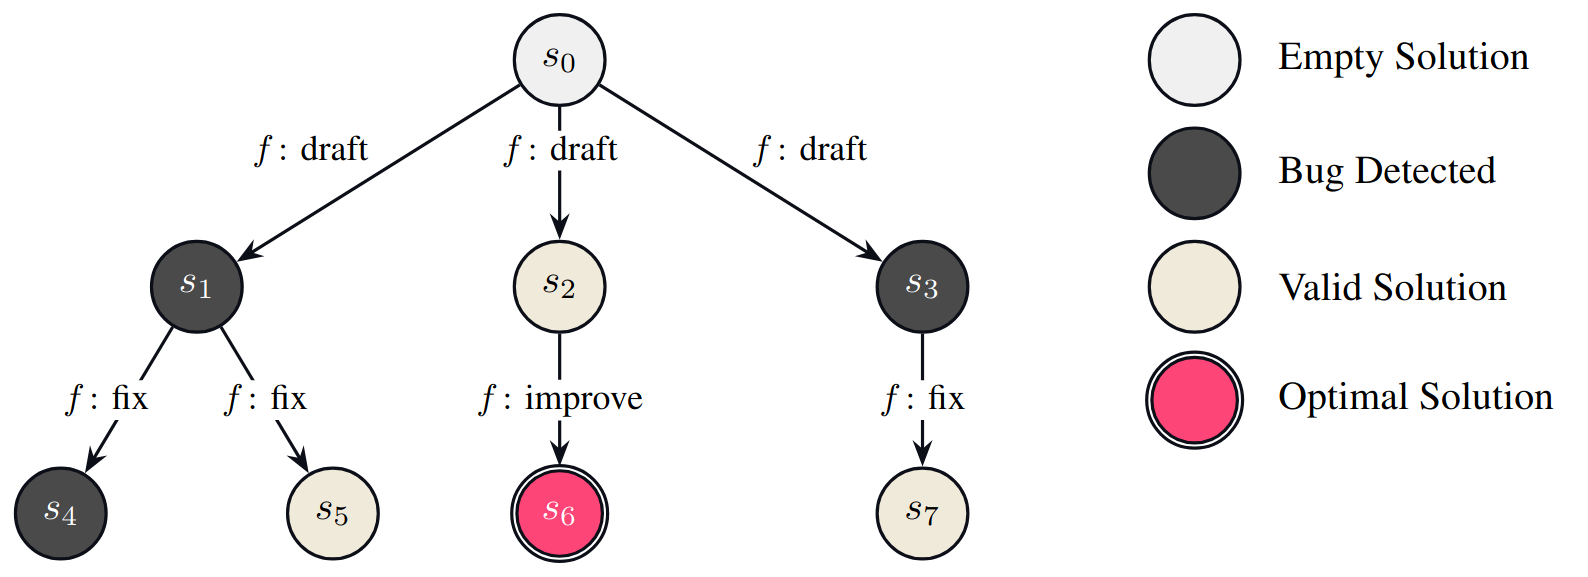
\includegraphics[width=0.8\linewidth]{images/aide-solution-tree.png}
%     \caption{A sample solution tree for AIDE, illustrating the drafting, fixing, and improvement steps. (Source: Schmidt et al., 2025, p. 4)}
%     \label{fig:enter-label}
% \end{figure}

% The Solution Tree ($T$): This is all discovered/proposed solutions (Python code scripts) and the improvement attempts (edges linking them) stored in a tree structure. The root solution ($s_0$) is typically an empty script, a node with value 'None'.

% Evaluator ($h$): This is a stateless function that takes a solution script as input and returns a scalar score (e.g., validation accuracy, loss). This score guides the search process. this evaluator is composed of a code interpreter that executes the code, then another LLM then takes the execution result (the trace back) and produces a structured output via function calling. this particular role is considered stateless since it always produce the same score, and it does not include past attempts in its evaluation, and this is important in the overall tree search for the best solution as every node or possible solution is evaluated primary on this.

% Search Policy ($\pi$): AIDE uses a simple, hard-coded search policy that determines the next step or next action. Based on the current state of the solution tree, it decides to:

% 1. Draft a new initial solution (if a desired number of diverse starting points hasn't been reached).

% 2. Debug a buggy node (if it's within a certain debug depth).

% 3. Improve an existing, non-buggy solution (typically targeting the current best-performing one).

% This policy has practical heuristics, such as initially exploring diverse solutions and then iteratively refining the most promising ones, while also limiting attempts to fix persistently broken solutions. Although this might be the most obvious area of improvement in the AIDE pipline, weather that was using a learned model that guides this search, the nature of the problems that small open source models have is largely not caused by the search heuristic, rather it is more fundamental in terms of ability to generate valid code in the first place, or correct usage of libraries and APIs.

% Coding Operator ($F$): This is the LLM itself as it proposes new scripts. It has three main entry points, each with specialized prompts:

% Drafting: Create a completely new solution `exploration`. The LLM is prompted to outline a plan to solve the problem (e.g., specify a neural network architecture and feature engineering ideas) and then generate a single-file Python program implementing that plan. These are then separated using regular expressions.

% Debugging: Repairing buggy solutions by inspecting error logs and execution traces. It attempts to fix issues like broken imports or incorrect tensor dimensions while preserving the overall approach.

% Improving: Called when a valid, non-buggy solution exists but could benefit from modifications (data preprocessing changes, architectural adjustments, or optimization tweaks and hiperparameter tuning). The LLM is prompted to propose a single `atomic` change, such as switching an optimizer or adding a regularization technique, so its impact on performance can be directly measured.

% Finally, to manage the LLM's context window and avoid `prompt explosion' from an  the growing history being fed to the model during the debugging and improvement phases, AIDE uses a summarization operator. Instead of appending all historical logs, this operator selectively extracts relevant information from the solution tree, such as Performance metrics (accuracy, AUC-ROC, etc.), Hyperparameter settings from previous attempts, Relevant hints for debugging (e.g., misaligned array shapes from trace-backs), This concise summary allows each code revision to be somewhat stateless yet guided by prior information, maintaining efficiency.

% Data Preview in Coding Prompts: AIDE also includes a small, static `data preview' in its coding prompts, providing the LLM with basic knowledge of the dataset's size or feature layout without needing extensive exploratory data analysis (EDA) at each step. As there is a code interpreter part of this iterative process, this Data preview tells the model exactly where and how the data is organized, and where to save its output or `submission.csv`

% The choice of AIDE as the foundational scaffold for this research is deliberate. It is open-source , it allows for the modification and integration of the inference-time scaling methods (self-consistency and self-reflection, etc) that are central to our work. Furthermore, AIDE's design, which explicitly models ML engineering as an iterative code optimization and tree search process powered by an LLM, provides a structured environment to study the effects of these techniques. It is established and proven to work effectively in solving ML tasks, as demonstrated in its original paper and subsequent evaluations on benchmarks like MLE-Bench, offers a great platform for experimentation. 

% AIDE has been tested and evaluated only using lagre-scale propriety LLMs, and our aim is to investigate how inference-time strategies can enhance AIDE's problem-solving capabilities, particularly its ability to make an open source, small-scale LLM generate more robust and higher-performing solutions on the challenging task like Machine learning Engineering.


% \section{MLE-Bench}
% To assess the performance of the enhanced aide scaffold we developed, we utilize the newly released MLE-bench, a benchmark for measuring how well AI agents perform at machine learning engineering, it is composed of 75 kaggle competitions, curated carefully from the Metakaggle dataset that contains around 5000 Kaggle competitions.
% This benchmark is designed specifically to be a benchmark for evaluating the performance of AI agents at machine learning engineering. MLE-Bench vary in category, scale, and complexity. This benchmark is designed not merely to test isolated skills, but to measure an agent's capacity for autonomous, end-to-end problem-solving—a workflow that spans model creation, training, evaluation, and iterative refinement.

% While MLE-Bench is a recent development, it is built upon a foundation of prior work aimed at evaluating LLMs coding and agentic abilities. Benchmarks like APPS (Hendrycks et al., 2021) and early evaluations of models such as Codex (Chen et al., 2021) have been used to measure general coding competence. The choice of MLE-Bench, and its particular relevance to this thesis, lies in its focus on tasks that are both representative of modern industry practices and known to be challenging for current AI systems, it offers a more specialized and demanding evaluation. However, it is very big benchmark, and evaluating on the 75 competitions is computationally infeasable for this thesis, hece, we opted for a subset of the benchmark,
% The core design of MLE-Bench is mostly around its task selection. The 75 selected competitions present an extremly difficult challenge for any coding agent. Essentially, MLE-Bench provides an offline Kaggle competition environment. For context, Kaggle is a platform that hosts data science and ML competitions where participants build predictive models to solve real-world challenges, competing for the best score on predefined metrics and earning rankings on a leaderboard. Top performers are often awarded monetary prizes, in addition to recognition with a bronze, silver, or gold medals. MLE-Bench adopts a similar structure to Kaggle, allowing for a realistic comparison of agent performance against historical human achievements 'offline leaderboard. The final results in this benchmark are often presented in terms of the average number of medals an agent would have won, determined by comparing its solution's metric on an unseen test set against the saved leaderboard from the original Kaggle competition.



% \section{Experiment Setup}

% To provide a rigorous and reliable evaluation of the inference-time strategies proposed in this thesis, a carefully designed experimental setup is essential. This section outlines the benchmark competitions, the baselines for comparison, the specific metrics used for evaluation, and the overall experimental procedure. The primary goal is to establish a solid evaluation framework that can take a given agent configuration as input and produce clear, quantitative metrics to determine its effectiveness relative to other methods.

% 1. Benchmark Competitions

% The foundation of our evaluation is a representative subset of competitions from the official MLE-Bench framework. While the full MLE-Bench is extensive, running experiments on all 75 competitions is computationally prohibitive for this project. Therefore, I have selected a curated subset of 10 competitions from the 'lite' complexity category. This choice was driven by several factors:

% Diversity: The selected competitions span 6 distinct machine learning categories, ensuring that our evaluation is not biased towards a single problem type. This diversity is crucial for assessing the general applicability of the proposed inference strategies.

% Feasibility: By focusing on 'lite' competitions, which are relatively lightweight in terms of data size and complexity, our experiments can focus on the quality of the agent's problem-solving process rather than being constrained by the technical overhead of handling massive datasets.

% Representativeness: This subset is a good representation of the full 'lite' category and provides a strong, empirical basis for evaluation.

% Flexibility: The chosen set is flexible enough to be extended in future work, either by including more competitions from the 'lite' category for a full standard comparison or by adding selected 'medium' complexity tasks to further test the limits of our methods.

% The 10 competitions selected for this benchmark are detailed in Table \ref{tab:competitions}.

% % \begin{table}[h!]
% % \centering
% % \caption{Selected Benchmark Competitions from MLE-Bench 'Lite' Category}
% % \label{tab:competitions}
% % \begin{tabular}{ll}
% % \hline
% % \textbf{Competition Name} & \textbf{Category} \ \hline
% % aerial-cactus-identification & Image Classification \
% % leaf-classification & Image Classification \
% % spooky-author-identification & Text Classification \
% % random-acts-of-pizza & Text Classification \
% % tabular-playground-series-may-2022 & Tabular \
% % nomad2018-predict-transparent-conductors & Tabular \
% % denoising-dirty-documents & Image to Image \
% % text-normalization-challenge-english-language & Sequence to Sequence \
% % text-normalization-challenge-russian-language & Sequence to Sequence \
% % mlsp-2013-birds & Audio Classification \ \hline
% % \end{tabular}
% % \end{table}

% 2. Baselines for Comparison

% To properly contextualize the performance of our proposed methods, we will benchmark them against a diverse set of established baselines. The aim is twofold: first, to prove that our strategies provide a meaningful improvement over a standard open-source model, and second, to demonstrate that these strategies make open-source models competitive with both closed-source counterparts and human experts.

% The baselines are summarized in Table \ref{tab:baselines}.

% % \begin{table}[h!]
% % \centering
% % \caption{Baselines for Performance Comparison}
% % \label{tab:baselines}
% % \begin{tabular}{lll}
% % \hline
% % \textbf{Baseline} & \textbf{Type} & \textbf{Reason for Inclusion} \ \hline
% % \textbf{AIDE + GPT-4o} & CS / High-Capability & Represents a strong, widely-used frontier model. \
% % & & Provides a high-water mark for performance. \ \
% % \textbf{AIDE + o4-mini} & CS / Reasoning-Optimized & Assumed to be a cost-effective, state-of-the-art reasoning \
% % & & model from OpenAI. Serves as a key SOTA reference. \ \
% % \textbf{AIDE + Llama 3.1 (405B)} & OS / High-Capability & A top-tier open-source model. Outperforming this \
% % & & demonstrates the power of our strategy. \ \
% % \textbf{Our Model + Default AIDE} & OS / Ablation & \textbf{Critical baseline.} This isolates the performance gain \
% % & & attributable specifically to our inference strategies, \
% % & & by removing them from our chosen model. \ \
% % \textbf{Human Performance} & Human Eval & Provides real-world context by comparing agent scores \
% % & & to the original Kaggle leaderboards. \ \hline
% % \end{tabular}
% % \end{table}

% 3. Evaluation Metrics

% To capture a holistic view of agent performance, we will use a suite of metrics inspired directly by the MLE-Bench and AIDE papers. These metrics evaluate an agent's ability to produce functional code, understand the task requirements, and ultimately generate an optimal solution.

% Code and Submission Generation: These metrics assess the fundamental ability of the agent to generate working code and complete the task.

% Valid Code Rate (\%): The number of steps that produce a valid, executable script divided by the total number of steps, averaged across seeds and competitions. A higher rate indicates a stronger fundamental code generation capability.

% Valid Submission Rate (\%): The percentage of independent runs (i.e., per seed, per competition) that successfully produce a submission file that passes the benchmark's validity checks. This is a stricter measure of task completion.

% Performance Against Human Baselines: Once a valid submission is produced, its quality is scored against the historical human leaderboard.

% Above Median (\%): The percentage of competitions where the agent's best score is strictly better than the median score achieved by human participants.

% Any Medal (\%): The percentage of competitions where the agent's best score is high enough to have earned a bronze, silver, or gold medal according to official Kaggle rules. This is our headline metric for overall success.

% The final results for each agent configuration will be presented in a summary table, as shown in the template in Table \ref{tab:results_template}.

% % \begin{table}[h!]
% % \centering
% % \caption{Template for Aggregated Results Table}
% % \label{tab:results_template}
% % \begin{tabular}{lccc}
% % \hline
% % \textbf{Model + Method} & \textbf{Valid Submission (\%)} & \textbf{Above Median (\%)} & \textbf{Any Medal (\%)} \ \hline
% % AIDE + o4-mini & X% 
% % ±
% % ±
% %  Y & X% 
% % ±
% % ±
% %  Y & X% 
% % ±
% % ±
% %  Y \
% % Our Model + Strategy 1 & X% 
% % ±
% % ±
% %  Y & X% 
% % ±
% % ±
% %  Y & X% 
% % ±
% % ±
% %  Y \
% % Our Model + Default AIDE & X% 
% % ±
% % ±
% %  Y & X% 
% % ±
% % ±
% %  Y & X% 
% % ±
% % ±
% %  Y \ \hline
% % \end{tabular}
% % \end{table}

% 4. Experimental Procedure

% To ensure a fair and repeatable evaluation, all experiments are conducted using a standardized protocol within a consistent environment.

% Environment: All runs are executed within a Dockerized environment to ensure consistency. AIDE is configured with fixed hyperparameters for all methods (e.g., 20 steps per attempt, 5 initial drafts).

% Execution: For each of the 10 competitions, every agent configuration ("Method") is run for k=3 independent attempts (seeds). This helps account for the inherent stochasticity of LLMs.

% Data Collection: After each run, we automatically collect the raw data, including whether a valid submission was generated and its corresponding score.

% Metric Calculation: Using the collected data, we calculate the flags for Valid Submission, Above Median, and Any Medal for each run.

% Aggregation: These flags are then aggregated. For metrics like Above Median and Any Medal, we consider a competition "solved" if at least one of the three seeds was successful (a pass@3 approach). The final percentages are averaged across the 10 competitions, with results reported as mean ± standard error.

% This standardized pipeline ensures that as we introduce and test new inference-time strategies, the results are directly and fairly comparable to our established baselines.



% % This is essentially what AIDE’s “solution tree” does conceptually – it navigates a solution space tree by proposing variations and seeing which yields better scores. Another formulation is the Tree-of-Thoughts
% % approach (Yao et al., 2023) where the model can propose multiple thoughts (steps of a solution)

% % This is somewhat what AIDE does by default (running the full training code to get a score), but one could go further and allow fine-grained tool use: the agent could execute just a part of the code (say a data pre-processing step) to inspect intermediate results, or call a library function to check documentation, etc. Another tool is a web browser or documentation fetcher, useful if the coding problem needs external knowledge
% % (though MLE-bench specifically disallows internet to prevent cheating). Still, 

% % For instance, in
% % OpenAI’s tests, they tried different “scaffolds”: AIDE, ResearchAgent, CodeAct, etc., each of which
% % structures the LLM’s process differently. 

% % AIDE’s self-reflection is essentially
% % an internal critic role given to the same model. We could also have a different model entirely
% % serve as the critic – for instance, use a 13B model to generate code and a more reliable 13B or
% % a set of heuristic rules to review it. This two-model system was not explicitly used in AIDE (to
% % our knowledge, AIDE uses one model for everything), but it’s a viable ITS approach: compose
% % multiple smaller experts rather than rely on one monolith. Each expert at inference time does
% % part of the task. 

% % search algorithms to explore solution space, tool use to gain information or verify outputs during generation, and modular agent frameworks that break the task into
% % pieces handled sequentially. These methods have proven effective: for example, using a Process Reward
% % Model + search enabled a 3B model to outperform a 70B model on a math benchmark, and
% % self-debugging allowed models to fix errors that they would otherwise miss. Importantly, most of these
% % techniques do not require fine-tuning the base model – they work by manipulating the inference
% % process (through prompting, iterating, or orchestration). Some advanced methods do introduce learned
% % components (e.g. training a verifier network, or fine-tuning the model to better utilize reflections), which blurs the line between pure inference-time and training. We’ll discuss a few such cases as well, but
% % the primary focus is on what can be done on the fly with an off-the-shelf model. The ultimate goal of
% % 5these strategies is well captured by OpenAI’s notion of “self-verification”, where the model can reliably
% % check its own work instead of relying on a giant ensemble or an external judge. In the next section,
% % we propose concrete techniques from these categories that AIDE could adopt to further empower its
% % small-model code generation in the ML domain.
% % **EITHER SPEAK ABOUT AIDE AND MLE BENCH HERE OR IN THE METHODS SECTINO** % You do not need to have exactly 4 chapters.
%                  % It is probably a good minimum, with 5 chapters 
%                  % average, and 7 chapters might be a maximum.
% % \chapter{Summary of Results}

% This chapter provides a concise overview of the experimental results, presenting the key aggregate performance metrics and empirical code generation capabilities for the evaluated agent configurations on the MLE-Bench subset.

% \section{Aggregate Performance Summary}

% Table \ref{tab:summary_aggregate} summarizes the overall performance of each model configuration, focusing on key metrics such as Valid Submission Rate (VSR), Above Median Rate (AMR), and Any Medal Rate (Pass@3). Made Submission is also included as a primary pipeline success indicator.

% \begin{table}[h!]
%     \centering
%     \caption{Summary of Aggregate Performance Metrics}
%     \label{tab:summary_aggregate}
%     % Using tabularx to make the table fit within the text width
%     \begin{tabularx}{\textwidth}{p{4.5cm} *{4}{>{\centering\arraybackslash}X}}
%         \toprule
%         Method                      & Made Submission (\%) & Valid Submission (\%) & Above Median (\%) & Any Medal (Pass@3 \%) \\
%         \midrule
%         \textbf{AIDE} & & & & \\
%         AIDE + o1-preview          & - & - & - & - \\
%         AIDE + GPT-4-turbo         & 73.3 $\pm$ 3.3 & 63.3 $\pm$ 3.3 & 20.0 $\pm$ 5.8 & 6.7 \\ % Pass@3 based on provided table
%         AIDE + gpt-4o-mini         & 76.7 $\pm$ 2.4 & 63.3 $\pm$ 2.4 & 26.7 $\pm$ 2.4 & 10.0 \\ % Pass@3 based on provided table
%         AIDE + DeepSeek-7B (Base)  & 23.3 $\pm$ 3.3 & 20.0 $\pm$ 0.0 & 0.0 $\pm$ 0.0 & 0.0 \\ % Pass@3 based on provided table
%         AIDE + DeepSeek-7B + SR    & - & - & - & - \\
%         AIDE + DeepSeek-14B (Base) & 73.3 $\pm$ 2.4 & 60.0 $\pm$ 4.1 & 10.0 $\pm$ 4.1 & 10.0 \\ % Pass@3 based on provided table
%         AIDE + DeepSeek-14B + SR   & - & - & - & - \\
%         AIDE + DeepSeek-32B (Base) & 76.7 $\pm$ 3.3 & 63.3 $\pm$ 3.3 & 33.3 $\pm$ 3.3 & 20.0 \\ % Pass@3 based on provided table
%         AIDE + DeepSeek-32B + SR   & - & - & - & - \\
%         \midrule
%         \textbf{Human Performance} & - & - & 50.0 & 12.4 \\
%         \bottomrule
%     \end{tabularx}
%     \caption*{\textbf{Note}: Metrics are mean $\pm$ standard error of the mean, averaged across 10 competitions and 3 seeds, except for Pass@3 which is the percentage of competitions with at least one medal across 3 seeds. SR denotes Self-Reflection strategy. Entries marked '-' indicate data was not available in the provided context.}
% \end{table}

% \section{Empirical Code Generation and Submission Attempt Summary}

% Table \ref{tab:summary_empirical} provides a summary of the average empirical metrics, highlighting the agent's code generation capabilities and pipeline progression based on Valid Code Generation Rate (VCGR), CSV Submission Attempt Rate (CSAR), Average Steps to First Working Output (StepsToWO), and Average Code Quality.

% \begin{table}[h!]
%     \centering
%     \caption{Summary of Empirical Code Generation and Submission Attempt Metrics}
%     \label{tab:summary_empirical}
%     % Using tabularx to make the table fit within the text width
%     \begin{tabularx}{\textwidth}{p{4.5cm} *{5}{>{\centering\arraybackslash}X}}
%         \toprule
%         Metric                     & AIDE + gpt-4o-mini & AIDE + GPT-4-turbo & AIDE + DeepSeek-7B (Base) & AIDE + DeepSeek-14B (Base) & AIDE + DeepSeek-32B (Base) \\
%         \midrule
%         VCGR (\%)                   & 40.53              & 40.40              & 3.73                      & 24.83                      & 25.63                      \\
%         CSAR (\%)                   & 41.47              & 41.87              & 4.93                      & 29.24                      & 26.50                      \\
%         Avg. Steps to First WO     & 9.77               & 12.00              & 28.77                     & 13.86                      & 13.56                      \\
%         Avg. Code Quality (1-10)    & 5.76               & 5.86               & 3.66                      & 5.00                       & 5.26                       \\
%         \bottomrule
%     \end{tabularx}
%     \caption*{\textbf{Note}: Metrics are averaged over all available runs (typically 10 competitions $\times$ 3 seeds). VCGR is the percentage of steps generating valid code. CSAR is the percentage of steps attempting a CSV submission. StepsToWO is the average number of steps to the first working output (using the \texttt{StepsToWO\_inf\_replaced} value from the source data). Avg. Code Quality is on a scale of 1--10. Data for models with the Self-Reflection strategy was not available in the provided aggregate empirical summaries.}
% \end{table} % Conclusion is usually a chapter itself. 
% \chapter{Discussion and Conclusion}

This chapter provides a concise overview of the experimental results, presenting the key aggregate performance metrics and empirical code generation capabilities for the evaluated agent configurations on the MLE-Bench subset.

\section{Aggregate Performance Summary}

Table \ref{tab:summary_aggregate} summarizes the overall performance of each model configuration, focusing on key metrics such as Valid Submission Rate (VSR), Above Median Rate (AMR), and Any Medal Rate (Pass@3). Made Submission is also included as a primary pipeline success indicator.

\begin{table}[h!]
    \centering
    \caption{Summary of Aggregate Performance Metrics}
    \label{tab:summary_aggregate}
    % Using tabularx to make the table fit within the text width
    \begin{tabularx}{\textwidth}{p{4.5cm} *{4}{>{\centering\arraybackslash}X}}
        \toprule
        Method                      & Made Submission (\%) & Valid Submission (\%) & Above Median (\%) & Any Medal (Pass@3 \%) \\
        \midrule
        \textbf{AIDE} & & & & \\
        AIDE + o1-preview          & - & - & - & - \\
        AIDE + GPT-4-turbo         & 73.3 $\pm$ 3.3 & 63.3 $\pm$ 3.3 & 20.0 $\pm$ 5.8 & 6.7 \\ % Pass@3 based on provided table
        AIDE + gpt-4o-mini         & 76.7 $\pm$ 2.4 & 63.3 $\pm$ 2.4 & 26.7 $\pm$ 2.4 & 10.0 \\ % Pass@3 based on provided table
        AIDE + DeepSeek-7B (Base)  & 23.3 $\pm$ 3.3 & 20.0 $\pm$ 0.0 & 0.0 $\pm$ 0.0 & 0.0 \\ % Pass@3 based on provided table
        AIDE + DeepSeek-7B + SR    & - & - & - & - \\
        AIDE + DeepSeek-14B (Base) & 73.3 $\pm$ 2.4 & 60.0 $\pm$ 4.1 & 10.0 $\pm$ 4.1 & 10.0 \\ % Pass@3 based on provided table
        AIDE + DeepSeek-14B + SR   & - & - & - & - \\
        AIDE + DeepSeek-32B (Base) & 76.7 $\pm$ 3.3 & 63.3 $\pm$ 3.3 & 33.3 $\pm$ 3.3 & 20.0 \\ % Pass@3 based on provided table
        AIDE + DeepSeek-32B + SR   & - & - & - & - \\
        \midrule
        \textbf{Human Performance} & - & - & 50.0 & 12.4 \\
        \bottomrule
    \end{tabularx}
    \caption*{\textbf{Note}: Metrics are mean $\pm$ standard error of the mean, averaged across 10 competitions and 3 seeds, except for Pass@3 which is the percentage of competitions with at least one medal across 3 seeds. SR denotes Self-Reflection strategy. Entries marked '-' indicate data was not available in the provided context.}
\end{table}

% \section{Empirical Code Generation and Submission Attempt Summary}

% Table \ref{tab:summary_empirical} provides a summary of the average empirical metrics, highlighting the agent's code generation capabilities and pipeline progression based on Valid Code Generation Rate (VCGR), CSV Submission Attempt Rate (CSAR), Average Steps to First Working Output (StepsToWO), and Average Code Quality.

% \begin{table}[h!]
%     \centering
%     \caption{Summary of Empirical Code Generation and Submission Attempt Metrics}
%     \label{tab:summary_empirical}
%     % Using tabularx to make the table fit within the text width
%     \begin{tabularx}{\textwidth}{p{4.5cm} *{5}{>{\centering\arraybackslash}X}}
%         \toprule
%         Metric                     & AIDE + gpt-4o-mini & AIDE + GPT-4-turbo & AIDE + DeepSeek-7B (Base) & AIDE + DeepSeek-14B (Base) & AIDE + DeepSeek-32B (Base) \\
%         \midrule
%         VCGR (\%)                   & 40.53              & 40.40              & 3.73                      & 24.83                      & 25.63                      \\
%         CSAR (\%)                   & 41.47              & 41.87              & 4.93                      & 29.24                      & 26.50                      \\
%         Avg. Steps to First WO     & 9.77               & 12.00              & 28.77                     & 13.86                      & 13.56                      \\
%         Avg. Code Quality (1-10)    & 5.76               & 5.86               & 3.66                      & 5.00                       & 5.26                       \\
%         \bottomrule
%     \end{tabularx}
%     \caption*{\textbf{Note}: Metrics are averaged over all available runs (typically 10 competitions $\times$ 3 seeds). VCGR is the percentage of steps generating valid code. CSAR is the percentage of steps attempting a CSV submission. StepsToWO is the average number of steps to the first working output (using the \texttt{StepsToWO\_inf\_replaced} value from the source data). Avg. Code Quality is on a scale of 1--10. Data for models with the Self-Reflection strategy was not available in the provided aggregate empirical summaries.}
% \end{table} % You may have more chapters. (Use e.g. git add FILE)
% This is where we stop counting pages.
% Acknowledgements and References are not counted.
%-----------------------------------------------------------------------------
% See the acknowledgement.tex file and follow the instructions there.

%-----------------------------------------------------------------------------
% Note the errata page is not for now, it is for use during the examination.
% Not that you're going to have any errata.
%-----------------------------------------------------------------------------
% THE BIBLIOGRAPHY 
% Bibliography styles define how the bibliography is 
% listed and formatted. This is part of the AIMS house
% style and is only changed under exceptional circumstances



% % ----------------------------------------------------------------------------
% % An AIMS Essay can use the sectioning commands "\chapter", "\section",
% % "\subsection". No "\subsubsection", "\paragraph", etc. They are disabled.
% % 
% % For Theorems and such, use the environments defined here:
% % \begin{thm}...\end{thm} (or "lem", "defn", etc)
% % 
% % We put the number to the left of the Theorem heading.
% \swapnumbers 
% % 
% % Theorems are in italics.
% \theoremstyle{plain}
% \newtheorem{thm}[subsection]{Theorem}
% %
% % Rest is not in italics.
% \theoremstyle{definition} 
% \newtheorem{lem}[subsection]{Lemma}
% \newtheorem{cor}[subsection]{Corollary}
% \newtheorem{conj}[subsection]{Conjecture}
% \newtheorem{pro}[subsection]{Proposition}
% \newtheorem{exa}[subsection]{Example}
% \newtheorem{defn}[subsection]{Definition}
% \newtheorem{rem}[subsection]{Remark}
% % 
% % If you have no theorems, but a lot of equations, maybe the
% % following two lines are good. Beware of corresponding Equation
% % and Example numbers though! Number equations by sections.
% % 
% \numberwithin{equation}{section}
% %
% %-----------------------------------------------------------------------------
% % Abstracts are usually written in English, with a version in your
% % mother tongue underneath.
% %
% % French, Igbo, Malagasy, etc. students use normal LaTeX
% % for special characters, for example \'{e}
% %
% % Amharic students use LibreOffice to write Amharic,
% % export and include a figure.
% %
% %\begin{RLtext}    
% %Here is where the arabic text goes.
% %You can just type it with an arabic keyboard
% %\end{RLtext}\\
% %-----------------------------------------------------------------------------
 
% % Your own command shortcuts can go here
% % keep them clearly separate from other sections of the preamble
% % It is good style to have only a few of these so that
% % we can read one another's code. If you have to many, 
% % then your code does not compile in someone else's template easily,
% % and it makes it harder to read. These definitions are only
% % meant for very often-used commands to save typing; Examples:
% %
% %\newcommand {\be}{\begin{equation}}
% %\newcommand {\ee}{\end{equation}}
% %\newcommand {\C}{\mathbb{C}} % Complex
% %\newcommand {\Z}{\mathbb{Z}} % Integers
% %\newcommand {\R}{\mathbb{R}} % Real
% %\DeclareMathOperator{\sech}{sech} % declaring new math operators like \sin.
% %  
% %-----------------------------------------------------------------------------
% % Title & Author


% % On this page you must have NO full-word capitalizations, bold, or colour. 
% % All AIMS research projects per year have the same title page.
% % In English your family name is written last, i.e. Firstname LASTNAME
% % English Capitalization, not as in some Francophone countries where
% % you write LASTNAME, Firstname.
% % Put your AIMS email address only please, for consistency,
% % not gmail or some other webmail address.
% \title{The Essay Title goes here Rafa\l Rafa\L{} test}
% % Your name must be in English Capitalisation with no comma, 
% % and the Family name comes last.
% \author{Firstname Middlename Familyname (email@aims.ac.za)\\
% % Then in the MAIN BODY use this:          


% %%%%%%%%%%%%%%%%%%%%%%%%%%%%%%%%%%%%%
% % Amharic students speak to me about how to add your name in your own alphabet.
% % Everything here is prescribed; do not enter bold or ALL CAPS here,
% % it will not be accepted.
% African Institute for Mathematical Sciences (AIMS)\\
% \\
% % Example1
% {\small Supervised by: Title Firstname Lastname}\\
% {\small Institute of Supervisor, Country}%\\
% % For second/more supervisors, continue with another line, e.g.
% % {\small and Dr So And-so}
% % {\small University of Life, Country}
% % Don't put the department, it becomes too long.
% }
% \date{{\small 24 October 2024}\\%
%   {\scriptsize\it Submitted in partial fulfillment of 
%     a structured masters degree at AIMS South Africa}\\%
%   \vspace{0.5cm}{\includegraphics{images/AIMS_SA_Logo.pdf}}}
% %-------------------------------------------------------------------------
% \begin{document}
% %\selectlanguage{english}
% \pagestyle{empty}
% \maketitle
% % All other files are included via \input. 
% % To compile in texmaker while viewing any of those
% % without having to switch back, use
% %   Options > Define Current Document as 'Master Document'
% % To not have to close a PDF, remove viewpdf from quickbuild 
% % and open the PDF (once) manually: it will auto-refresh or with control-r
% % 
% %-------------------------------------------------------------------------
% % The abstract is the first thing we want to see. No acknowledgements or 
% % dedications here. Fetch the abstract from a separate file.
% % Please write it in English and in your mother tongue.
% % An abstract should be less than half a page, so that both abstracts 
% % (that is both languages) fit onto one page.
% % We number roman numerals until the main body
% \pagenumbering{roman}
% \chapter*{Abstract}
\addcontentsline{toc}{chapter}{Abstract}
Recent findings suggest that reasoning strategies applied during inference can yield more significant performance gains in large language models (LLMs) than merely increasing their parameter scale. Furthermore, the emergence of advanced open-source LLMs, such as those distilled from DeepSeek-R1—which matches the performance of its closed-source counterpart, OpenAI-o1, offers new opportunities for exploration. Leveraging these more capable LLMs, we aim to evaluate their performance on complex tasks in machine learning engineering.

To this end, MLE-Bench provides an ideal benchmark. Designed to assess the machine learning engineering capabilities of AI agents, MLE-Bench comprises 75 diverse Kaggle competitions. Its primary goal is to comprehensively evaluate AI agents' ability to design and implement end-to-end machine learning pipelines, making it a rigorous testbed for these advanced LLMs.

This project examines the effectiveness of these distilled open-source LLMs when paired with inference-time reasoning strategies within and Agentic framework, on the machine learning tasks presented by MLE-Bench. The primary objective is to compare the performance of these open-source models with the more established LLM-based approaches outlined in the MLE-Bench paper. Ultimately, this work supports the broader vision of integrating LLM-based agentic systems into AI research workflows.

% \begin{otherlanguage}{arabic}
%     هذا هو الملخص العربي لمشروع البحث الخاص بك.
% \end{otherlanguage}
\vfill

\section*{Declaration}

I, the undersigned, hereby declare that the work contained in this research project is my original work, and that any work done by others or by myself previously has been acknowledged and referenced accordingly.
% \includegraphics[height=2cm]{images/signature.png} \newline \hrule

Asim Osman, 12 June 2025
% % Don't go typing out the contents.
% \tableofcontents
% \newpage
% % We switch to arabic numerals here where your page count starts
% % Essays must be close to 30 pages long *starting here* and up to and including
% % the conclcusion. It does not include the acknowledgements or references.
% % 
% % Figures may differ between topics, but they are not there
% % to fill the pages -- they must add meaning.
% % In general most figures should be 0.8 times the width of the page
% % (perhaps wider in total when two or three columns of figures)
% % See the example in chapter one for defining that. Be *consistent*
% % in your presentation of information.
% \pagenumbering{arabic}
% \pagestyle{myheadings}
% %-----------------------------------------------------------------------------
% % Each chapter goes in a separate file
% % Chapter titles are just examples
% % Always have a question
% % Note the Case Pattern used at AIMS
% \chapter{Introduction}

Over the last few years, advancements in large language models have primarily relied on scaling up the number of parameters alongside increasing dataset size and compute budgets. This strategy, often referred to as train-time compute scaling, has been remarkably effective, significantly and consistently improving model performance on tasks such as translation, general question answering, and sophisticated reasoning in mathematics and coding. However, the exponential growth in model size and the associated costs have become prohibitively expensive, pushing training budgets to the billion-dollar scale and raising concerns about resource sustainability, particularly as high-quality training data becomes scarcer.

Consequently, significant interest has shifted toward inference-time (or test-time) scaling techniques. Rather than focusing on costly retraining and larger models, inference-time scaling enhances existing models by dedicating additional computational resources during prediction. These methods enable models to "think longer" on challenging problems by dynamically generating multiple reasoning paths, employing voting mechanisms, or iteratively refining their outputs. Recent studies, such as DeepMind's compute-optimal scaling \citep{placeholder}, demonstrate how smaller models can achieve impressive performance through adaptive inference strategies, sometimes even outperforming substantially larger models.

In parallel with these developments, there has been a notable emergence of "reasoning" or "thinking" models, designed explicitly to enhance models' capabilities to reason through complex problems. A prime example is DeepSeek-R1, which explicitly trains models using reinforcement learning to produce long, structured chains of thought before providing an answer, enabling LLMs to systematically tackle tasks that were previously challenging even for large-scale models. DeepSeek released a series of small distilled models trained on reasoning datasets generated from the original R1 model, empowering them with remarkable reasoning capabilities and improving their performance relative to larger models.

Motivated by these developments, this work explores the promise of inference-time scaling techniques applied to small-scale language models-particularly those distilled from DeepSeek-that are specifically designed for coding and machine learning engineering tasks, areas still challenging even for frontier models. Smaller models have substantial advantages in accessibility, rapid deployment, and lower operational costs, but traditionally lack the advanced reasoning capabilities exhibited by larger models. Through systematic implementation and evaluation of strategies such as chain-of-thought prompting, iterative self-refinement, self-consistency, and other methods, this project aims to bridge the performance gap. Ultimately, this thesis evaluates the extent to which inference-time scaling can address complex tasks such as machine learning engineering. We demonstrate that, with carefully designed inference-time enhancements, small-scale models can significantly improve performance in complex coding and engineering contexts, presenting a viable and cost-effective alternative to training massive foundational models.

% \section{Introduction}
% The field of artificial intelligence is witnessing an unprecedented scaling race, where models with hundreds of billions of parameters demonstrate remarkable capabilities that seem to emerge from sheer computational scale. This phenomenon has created a stark divide in the AI landscape: while large proprietary models like GPT-4 and Claude achieve impressive performance on complex reasoning and coding tasks, smaller open-source alternatives lag significantly behind, creating substantial barriers to accessibility and democratization of AI capabilities.
% This performance gap is particularly pronounced in machine learning engineering tasks, where AI agents must not only write syntactically correct code but also reason about complex architectural decisions, debug intricate workflows, and navigate the nuanced requirements of end-to-end ML pipelines. Unlike general-purpose coding, ML engineering demands sophisticated reasoning about data preprocessing, model selection, hyperparameter optimization, and deployment considerations—capabilities that have remained largely the domain of expensive, proprietary models.
% The emergence of inference-time scaling (ITS) techniques offers a promising pathway to bridge this performance divide. Rather than requiring massive computational resources during training, ITS methods like chain-of-thought prompting, self-consistency, and iterative refinement allow smaller models to achieve enhanced performance by investing additional computation during inference. This paradigm shift suggests that the reasoning capabilities necessary for complex tasks might be accessible to open-source models through strategic application of ITS techniques.
% Recent advances in distilled reasoning models, particularly DeepSeek-R1's family of models ranging from 7B to 32B parameters, present an opportunity to test this hypothesis. These models demonstrate strong reasoning capabilities even at smaller scales, potentially providing the foundation needed for effective ML engineering agents when enhanced with appropriate ITS strategies.
% However, existing agentic frameworks have primarily focused on proprietary models accessed through APIs, leaving open-source implementations under-explored. While ITS techniques have been applied to coding tasks, their systematic integration with distilled reasoning models specifically for ML engineering remains largely uncharted territory. This gap represents both a technical opportunity and a practical necessity for organizations seeking to develop their own AI assistants without relying on expensive proprietary solutions.
% This thesis addresses these challenges by developing and evaluating an enhanced version of AIDE (AI-Driven Exploration), an open-source agentic scaffold specifically tailored for inference-time scaling with open-source models. Our approach integrates multiple ITS strategies—including self-consistency, iterative self-debugging, and modular task decomposition—with DeepSeek-R1 distilled models to create accessible ML engineering agents capable of autonomously tackling complex machine learning competitions.
% Contributions
% This work makes four key contributions to the field:

% High-Performance Open-Source Infrastructure: We develop a high-throughput parallel inference engine with multiprocess orchestration, enabling simultaneous experimentation across different models and tasks while maintaining competitive inference speeds for open-source deployments.
% Specialized Agentic Scaffold: We create an open-source agent framework specifically designed for the HuggingFace ecosystem, providing an alternative to proprietary API-based solutions and enabling broader accessibility to ML engineering automation.
% Systematic ITS Integration: We implement and evaluate multiple variants of AIDE, each incorporating different ITS strategies, providing a comprehensive exploration of inference-time scaling techniques for ML engineering tasks. These variants are made available as separate repository branches with a unified interface for strategy selection.
% Empirical Validation: We demonstrate that a 32B open-source model enhanced with appropriate ITS techniques can achieve performance comparable to GPT-4 Turbo on ML engineering tasks, reaching a practical level where the agent can autonomously solve Kaggle competitions end-to-end.

% Thesis Overview
% The remainder of this thesis is organized as follows. Chapter 2 provides essential background on agentic systems in research workflows, reviews the effectiveness of ITS techniques across domains, introduces the concept of agent scaffolding, and surveys existing benchmarks for evaluating ML engineering capabilities. Chapter 3 details our methodology, including the original AIDE framework, MLE-Bench evaluation protocols, and our systematic approach to integrating ITS strategies within the agentic scaffold. We discuss experimental design choices, cost considerations, baseline selection rationale, and provide detailed implementation insights for each ITS method. Chapter 4 presents comprehensive experimental results, including numerical evaluations of agent performance, analysis of observed behaviors, and discussion of failed approaches. Finally, Chapter 5 concludes with implications for future research and practical deployment considerations.
% Through this systematic investigation, we aim to demonstrate that the performance gap between proprietary and open-source models in ML engineering can be substantially reduced through careful application of inference-time scaling techniques, opening new avenues for accessible and democratized AI-driven automation in machine learning workflows. % Introduction is usually a chapter itself.
% \chapter{Background and Related Work}

\section{Background}

\subsection{Large Language Models (LLMs)}
Large Language Models (LLMs) are neural networks trained on extensive text datasets, capable of generating human-like text. Based primarily on the transformer architecture, these models utilize a straightforward predictive objective, leveraging enormous volumes of data to tackle complex problems and diverse natural language tasks [CITATION], including translation [CITATION], semantic analysis [CITATION], and information retrieval.

Recent advancements in LLMs, exemplified by models such as the GPT series [CITATION*3] and the Llama family [CITATION], have been driven by significant scale, reaching billions of parameters. This substantial scale has unlocked emergent abilities—advanced skills like reasoning and in-context learning—that smaller models typically do not exhibit. These emergent capabilities enable LLMs to solve arithmetic problems, answer intricate questions, and summarize complex passages, often without explicit task-specific training.

\subsection{Scaling Laws and Train-Time Compute}
Scaling lows shows how the performance of Large Language models improves in a predeictable way with the increase in the parameter size, training data and computationa; resources, openai ahs shown that LLMs performance as measured by metrics such as accuracy or perplexity follows a power low relationship with these scaling factors. Performance enhancements are steady yet exhibit diminishing returns as scale increases, motivating the development of increasingly larger models like PaLM and Chinchilla.

While scaling laws provided performance guarantees and drove a competitive race for building larger models, leading to current models in the hundreds of billions of parameters, practical limitations have surfaced. High-quality data is becoming scarce relative to growing model demands, and the significant costs and resource consumption associated with these models pose substantial challenges. Moreover, LLMs auto-regressive and token level prediction style is itself a limitation when it comes to complex reasoning tasks such as advanced mathematics or complex question answering. While recent years witnessed substantial developments in the models abilities, especially using post training and fine tuning, this requires massive computational resources and large scale datasets, encouraging researchers to to find cheaper approaches.

\subsection{Inference-Time Scaling (ITS)}
To address limitations associated with traditional scaling strategies, a new paradigm has emerged: inference-time scaling, also known as test-time scaling. Instead of allocating more resources to pretraining, this approach dynamically adjusts computational resources during inference, enabling models to "think longer" and thus handle more complex problems. Inference-time scaling involves techniques such as generating longer reasoning chains, sampling multiple possible answers, and iteratively refining outputs. This strategy has shown significant promise, allowing smaller models to surpass larger counterparts.

Techniques in inference-time scaling include:
\begin{itemize}
\item \textbf{Chain-of-Thought Prompting (CoT):} Encouraging models to explicitly generate intermediate reasoning steps.
\item \textbf{Iterative Self-Refinement:} Models iteratively identify and correct errors in their outputs.
\item \textbf{Self-Consistency:} Generating multiple independent outputs and selecting the most consistent result via voting.
\item \textbf{Verifier-Guided Search Techniques:} Utilizing reward-based verifiers or structured search methods to identify optimal answers from multiple generated solutions.
\end{itemize}

\subsection{Emergence of Reasoning Models}
Recent developments have highlighted the emergence of models focused on reasoninging specifically designed to enhanthe capabilities in multistep  logical and mathematical reasoning. These reasoning models utilize inference-time strategies like structured prompting, external tool usage, and systematic search without altering model weights. Techniques such as ReAct, PAL, Toolformer, and Tree-of-Thoughts have demonstrated significant improvements in reasoning abilities.

DeepSeek-R1 serves as a notable landmark, explicitly trained via reinforcement learning on structured reasoning datasets to generate coherent reasoning chains, significantly improving performance on complex reasoning tasks. DeepSeek's release of smaller distilled models, trained on datasets generated by R1, demonstrates the potential of distillation combined with structured inference strategies, achieving performance comparable or superior to larger models.

* the effect of rl training on producing long chains of thoughts
* the distilled models that were trained on the reasoning datata from R1 model

\subsection{Agentic Systems and Scaffolding}
"Scaffolding" reffers to code built up around an LLM in order to augment its capabilities. This does not typically include code which alters the LLM's internals, such as fine-tuning or activation steering. People use scaffolding because it can allow LLMs to use tools, reduce error rates, search for info, all of which make LLMs more capable.
Common types of scaffolds include:
Prompt templates: Perhaps the simplest scaffolds, "prompt templates" are just prompts with some blank sections to be filled in at runtime using some local data. E.g., a template like "You are a good assistant. The date is {INSERT DATE HERE}. Tell me how many days are left in the month." can be filled in with the current date before being used to prompt an LLM.
Retrieval Augmented Generation (RAG): For tasks which have some associated data, RAG is a way of automatically adding task-relevant info to prompts. RAG does this by looking for snippets of text/data in the database which are relevant to the user's prompt, and then adding those snippets to the prompt.
Search engines: Similar to RAG, giving an LLM access to a search engine lets it find info relevant to its prompt. Unlike RAG, the LLM decides what to search for and when.
Agent scaffolds: Scaffolds which try to make LLMs into goal-directed agents, i.e., giving an LLM some goal/task to perform, and ways to observe and act on the world. Usually, the LLM is put into a loop with a history of its observations and actions, until its task is done. Some agent frameworks give LLMs access to much more powerful high-level actions, which saves the AI from repeating many simple primitive actions and, therefore, speeds up planning.

Agent scaffolds are characterized by their capacity for perception, planning, and action within an environment, often governed by an iterative process that refines, reflects, and improves the solution over multiple cycles.

While agents scaffolds can be used in different domains and wide array of tasks, there has been increasing interest dedicated to developing agents capable of automating the machine learning research and engineering process. A notable example is the [AI scientist] system, which presents an end-to-end pipeline designed to automate the research workflow. Currently, data science, machine learning engineering, and more generally, coding agents and assistants have shown consistent improvements. as we now see agents like Gihub Capilot, Cognition | Introducing Devin, Cursor, or Claude code exhibit phenomenon coding abilities, but there is no significant progress in their open-source coding agents. 

The nature of coding problems presents a unique challenge for LLMs compared to other reasoning tasks, such as mathematics. In mathematical reasoning, there is often a single, unambiguously verifiable answer that can be derived through logical deduction. Conversely, generating a coding solution involves not only producing syntactically correct and executable code, but also navigating a vast solution space, where multiple functionally equivalent but structurally diverse implementations can exist. Crucially, the correctness and optimality of a coding solution often necessitate empirical validation through actual code execution and looking at traceback, rather than purely symbolic or logical verification. This inherent complexity, which demands iterative refinement and empirical testing, underscores the critical need for sophisticated agentic systems that can autonomously generate, execute, and iteratively refine solutions, even for highly capable foundational models.

\subsection{Relevance and Challenges in Coding and ML Engineering Tasks}
Machine learning engineering and coding tasks represent particularly challenging yet highly relevant applications for inference-time scaling due to their inherent complexity and precision requirements. Benchmarks like HumanEval, MBPP, and MLE-Bench exemplify these tasks, providing challenging evaluation contexts.

However, significant gaps persist in current research, such as limited open-source implementations and insufficient evaluation on realistic, complex coding tasks. This project explicitly addresses these gaps by systematically applying inference-time scaling techniques to small-scale distilled reasoning models, aiming to substantially enhance their performance and practical applicability in coding and ML engineering domains.

CITATION NEEDED
\section{Related Work}
% * systems such as aide, or any open source implemntaion
% * infercne time and how it improves small models
% *** I should find example for MATH of course ***
 

% \subsection{Inference-Time Scaling Techniques in the Coding Domain}

% The core idea in Inference-Time Scaling (ITS) for code generation is to allow a model to generate and evaluate multiple solutions or reasoning steps before finalizing an answer, much like a programmer iteratively writes, tests, and debugs code. This can enable smaller models to achieve results on par with much larger models by compensating with clever search and reasoning. Below is an overview of relevant ITS
% strategies in the context of code generation:

% \subsection{Multiple Sampling and Majority Voting}:
% The simplest form of test-time compute scaling is to sample many outputs and pick the best, much like an ensemble methods, this can be very effective as the LLMs output are not generally deterministic, and in theory. For coding, this might mean prompting a 7B model 10 times for a function implementation and then using a heuristic to choose among those attempts. Majority voting is one approach where if multiple samples converge on the same answer, that answer is taken as more likely correct. However, for complex coding problems (especially ones without a single "exact" answer), majority voting may not help much – if the model tends to make a consistent mistake, all samples will be wrong in the same way. Nonetheless, for simpler tasks (like leetcode-style problems with fixed outputs), self-consistency via voting can reduce random errors. 

% A more effective variant is "Best-of-N" selection, where instead of voting, the best candidate out of N is chosen based on an evaluation function. In coding, the evaluation function could be a set of unit tests or a code quality metric. For example, generate 5 different code solutions and then run all of them against some test cases, picking the one that passes the most tests. 

% This Best-of-N strategy was found to significantly improve math problem solving for small
% models when using an automated judge, and for code it can similarly boost correctness if a reliable evaluator is available. In practice, Best-of-N requires more inference runs (linear in N) and possibly running a reward model or tests to rank outputs, but it's a straightforward way to leverage extra compute. 

% Iterative Self-Improvement (Self-Reflection and Debugging): instead of generating
% many answers independently, another approach is to have the model improve
% a single solution by self-correcting mistakes in an iterative way. Techniques like self-
% reflection, as well as Self-Debugging and Reflexion feedback loops.

% The general pattern is: the model produces an initial solution, then the model (or another instance of it or another role controlled by the system prompt) is asked to inspect that solution for errors or flaws, and propose a fix, and this process repeats. In code generation, this mirrors the edit-compile-fix cycle programmers use. For example, Chen et al. (2023) introduced Self-Debugging, where an LLM is taught via examples to run the code (or at least simulate running it) and then asked to explain what the code is doing and identify any mistakes based on either runtime results or logical reasoning. Notably, their approach has the model look at execution results (e.g. error messages or failed tests) without human feedback, and then pinpoint the bug and fix it – effectively the model learns to debug itself. This yielded state-of-the-art results on several coding tasks, improving accuracy by up to 12\% on test-driven benchmarks by iteratively correcting errors.

% Reflexion, a recent idea for general reasoning, has the model generate a brief "reflec-
% tion" after a failed attempt, explaining what went wrong and how to adjust its next attempt. This reflection is then prepended to the next query so the model won't repeat the mistake. In coding, a similar approach can be used: after an unsuccessful run (say the model's code didn't produce a valid output or scored poorly), the agent can prompt the model to reflect: "Why did your solution perform poorly? What could be improved?" and use that answer to guide the next code revision.

% These self-corrective loops leverage the model's reasoning ability at inference time to gradually approach a correct solution, instead of having a perfect answer in one shot. 

% They are modular (generator + debugger) and don't require training new models – only cleverly designed prompt sequences and possibly a memory of past failures. This family of techniques is arguably one of the most promising for coding, because coding tasks naturally provide feedback (errors, test outcomes)
% that the model can learn from on the fly. 

% Search-Based Approaches (Beam Search, Tree-of-Thought, MCTS): Classic AI search algo-
% rithms can be applied at inference to guide the generation of code. Instead of treating the LLM as a black box that generates one solution, we can treat partial generations as states in a search tree. For instance, beam search is a technique where at each step of code generation, multiple possibilities are kept (`the beam') and the search explores several paths, not just the single most likely token sequence. In natural language generation this is tricky (due to the immense branching), but for structured tasks like code, researchers have attempted to incorporate it. A recent Hugging Face case study used beam search guided by a learned reward model to have a 1B model solve math problems step-by-step, expanding only the promising reasoning paths. 

% They further introduced Diverse Verifier Tree Search (DVTS), which explicitly encourages exploring diverse branches and uses a verifier to prune incorrect logic, preventing the search from converging on a wrong answer too early. Translating this to code: one could imagine generating different code approaches, one branch tries a neural network, another branch tries a gradient boosting model) and then evaluating both, continuing to refine whichever looks more promising. A search algorithm (DFS or BFS with pruning) explores combinations of these thoughts to find an overall successful solution. In coding tasks, a "thought" could be a high-level plan or a code snippet. By evaluating partial solutions (e.g., does the code run up to a certain point without error? Does a partial result look plausible?), an agent can systematically search for correct code. An Example is the S*framework augments parallel sampling with sequential debugging – generating multiple initial programs, then iteratively debugging each using execution feedback, and then selecting the best program at the end. It even uses adaptive test generation during selection: the LLM is asked to come up with specific inputs that differentiate two candidate programs, then it runs both programs on those inputs to see which one fails. Such adaptive search is quite advanced – effectively using the model to adversarially test its own outputs – and it was shown to let a 3B coder outperform models as large as 70B on code benchmarks. 

% In summary, search-based ITS techniques treat code generation as a search problem, leveraging multiple candidates and systematic exploration. These methods require more
% complex control logic (to manage the search and comparisons) and sometimes an external judge (which can be the model itself in a verifier role), but they can dramatically improve coverage of the solution space for tricky coding tasks.

% Tool-Assisted and Modular Reasoning: Another angle for inference-time improvement is
% giving the model external tools or modules to use while solving the problem. In coding, the
% most pertinent tool is a Python interpreter or execution environment. An agent with tool use ReAct paradigm or API toolformer approaches can decide to run a piece of code to see
% what happens and incorporate the result into its next step. For example, if the task is to write a function, the agent could generate a candidate, execute it on some test inputs, and observe the outputs or any exceptions, then adjust accordingly. for general coding tasks, letting the model search error messages or look up API usage could help a smaller model correct mistakes that it wouldn't know how to fix from training data alone. 

% A modular approach could also mean splitting the problem among specialized modules: for instance, a static analyzer module could lint the model's code for syntax errors or bad practices, and a test generator module could produce unit tests for the code. These modules might themselves be LLM prompts
% or traditional programs. Their feedback can then be fed into the model's next inference. Because
% these happen at inference time (no weights changed, just additional computation/feedback), they
% fall under ITS. example for this is to integrate a type-checker: the model writes Python code, run a type checker or even a lightweight symbolic execution to catch obvious misuses, then prompt
% the model with "The following variables might be undefined." By incorporating such tools in the loop,
% we can elevate a smaller model's performance – it doesn't need to have all knowledge internally
% if it can query an external helper. The ReAct framework demonstrated that even a single LLM
% agent can use tools effectively by interleaving reasoning and acting steps. In coding, this could
% mean the agent alternates between "think about how to solve" and "try running this piece" actions.
% Overall, tool-assisted inference allows modularizing the task and providing grounded feedback

% Agentic Scaffolding and Role Decomposition: Closely related to the above, many agent
% frameworks split the problem-solving into multiple roles or phases. An example would be a planner-executor paradigm: first prompt the LLM to write a high-level plan or pseudo-code, then in a second prompt have it implement that plan in actual code. This helps because the model can focus on logical planning in one stage and syntax in another, reducing cognitive load. Another example is having a separate critic agent: one model (or one chain of prompts) produces a solution, and another model (or later prompts of the same model) evaluates that solution. For coding, one might have: a "data scientist" agent that decides what model to use, a "coder" agent that writes the code, and a "tester" agent that runs and verifies the code. All could be orchestrated in one loop. Such modular, agentic strategies can dramatically improve outcomes since mistakes caught by one module can be fixed before the final answer. They don't require additional training if we use the same base model with different prompts, though they
% incur more inference calls. This approach has been demonstrated in other domains (for example, decomposition into sub-agents for math word problems). 
% In code generation, the AutoKaggle system (2024) uses a multi-agent workflow with different specialists collaborating on a competition problem. While complex, this shows promise in handling the many facets of ML engineering (data cleaning, modeling, hyperparameter tuning) through coordinated inference-time work.
% In summary, inference-time scaling in coding tasks includes sampling-based methods (generate many solutions, then filter or vote), iterative improvement (let the model refine its answer using feedback,
% either self-generated or from executing code).

% \subsection{Machine Learning Engineering Benchmarks and Automated research workflow}

% coding benchmarks like swebench*
% agent scaffolds like AutoML (H2O) etc *
% AI scientist, and kaggle agents.*


% Background and Related Work
% This chapter provides the technical foundation necessary to understand our approach to enhancing open-source machine learning engineering agents through inference-time scaling. We begin by establishing key concepts in large language models and their inference mechanisms, then explore how inference-time scaling has proven effective across various domains, before examining the specific challenges and opportunities in ML engineering automation.
% 2.1 Large Language Models and Inference
% 2.1.1 Foundation Models and Training Paradigms
% Large Language Models (LLMs) are transformer-based neural networks trained on vast text corpora to predict the next token in a sequence. The training process typically involves three stages: pretraining on diverse internet text to learn general language understanding, supervised fine-tuning on curated instruction-following datasets to align with human preferences, and reinforcement learning from human feedback (RLHF) to further refine behavior through preference optimization techniques like PPO or DPO.
% The pretraining phase establishes the model's foundational capabilities—its understanding of syntax, semantics, factual knowledge, and reasoning patterns. Fine-tuning then shapes how these capabilities are expressed, teaching the model to follow instructions, engage in dialogue, and perform specific tasks. This multi-stage approach has proven crucial for creating models that are both knowledgeable and helpful.
% 2.1.2 Inference Mechanisms and Decoding Strategies
% During inference, LLMs generate text through autoregressive decoding, where each token is predicted based on all previous tokens in the sequence. The decoding process involves several key parameters that significantly influence output quality and diversity:
% Temperature controls the randomness of token selection, with lower values (0.1-0.3) producing more deterministic outputs and higher values (0.7-1.0) increasing creativity and variability. Top-k sampling restricts token selection to the k most probable candidates, while top-p (nucleus) sampling dynamically adjusts the candidate pool based on cumulative probability mass, typically set between 0.8-0.95 for optimal balance between coherence and diversity.
% Beam search represents an alternative decoding strategy that maintains multiple candidate sequences simultaneously, exploring different paths through the probability space. While computationally more expensive than sampling methods, beam search can produce higher-quality outputs for tasks requiring careful reasoning or structured responses.
% The choice of decoding strategy and parameters can dramatically affect model performance on complex tasks, making inference-time optimization a critical consideration for practical applications.
% 2.1.3 Inference Engines and Deployment
% Modern LLM deployment relies on specialized inference engines that optimize memory usage, computational efficiency, and throughput. Popular frameworks include vLLM, which uses PagedAttention for efficient memory management, TensorRT-LLM for NVIDIA GPU optimization, llama.cpp for CPU inference, and Text Generation Inference (TGI) for production deployments.
% These engines implement various optimization techniques including dynamic batching, continuous batching, and KV-cache management to maximize hardware utilization. The choice of inference engine can significantly impact both the speed and cost of serving LLMs, particularly important considerations when deploying open-source models at scale.
% 2.2 Inference-Time Scaling: Beyond Training Scale
% While the field has long focused on scaling models through increased parameters and training compute, inference-time scaling (ITS) offers an alternative paradigm where additional computation during inference enhances model capabilities without requiring larger models or extended training.
% 2.2.1 Core ITS Techniques
% Chain-of-Thought (CoT) Prompting emerged as one of the first successful ITS techniques, where models are prompted to "think step by step" and show their reasoning process explicitly. This simple modification has shown remarkable effectiveness across mathematical reasoning, logical puzzles, and complex problem-solving tasks, often improving performance by 20-50% on challenging benchmarks.
% Self-Consistency extends CoT by generating multiple reasoning paths for the same problem and selecting the most frequent answer through majority voting. This technique leverages the insight that correct reasoning paths tend to converge on the same solution, while errors are more likely to be diverse and inconsistent. Self-consistency has demonstrated particular strength in mathematical and logical reasoning tasks.
% Iterative Self-Debugging allows models to review and refine their own outputs through multiple rounds of generation and critique. The model first produces an initial solution, then analyzes it for potential errors, and finally generates an improved version. This process can be repeated multiple times, with each iteration potentially improving solution quality.
% Self-Reflection involves explicit metacognitive processes where models evaluate their own reasoning, identify potential weaknesses, and adjust their approach accordingly. Unlike self-debugging, which focuses on error correction, self-reflection emphasizes strategic thinking about problem-solving approaches.
% 2.2.2 ITS Success Across Domains
% The effectiveness of ITS techniques has been demonstrated across numerous domains. In mathematical reasoning, techniques like self-consistency have improved performance on GSM8K and MATH benchmarks by substantial margins. In code generation, iterative refinement approaches have shown significant improvements on programming challenges, with models able to debug and optimize their initial solutions.
% Scientific reasoning tasks have also benefited from ITS, with models showing improved performance on physics problems, chemistry questions, and biological reasoning when given additional inference-time computation. The pattern is consistent: domains that require careful reasoning and step-by-step analysis tend to benefit most from ITS techniques.
% Notably, these improvements often scale predictably with inference-time compute, following power-law relationships similar to those observed in training-time scaling. This suggests that ITS represents a fundamental trade-off between model size and inference cost, potentially democratizing access to high-performance AI capabilities.
% 2.3 Reasoning Models and Distillation
% 2.3.1 The DeepSeek-R1 Family
% DeepSeek-R1 represents a significant advancement in open-source reasoning models, trained specifically to excel at step-by-step reasoning and complex problem-solving. The model family includes variants at 7B, 14B, and 32B parameters, each distilled from larger teacher models while maintaining strong reasoning capabilities.
% The distillation process preserves the reasoning patterns and step-by-step thinking that make larger models effective, compressing these capabilities into more accessible model sizes. This approach has proven particularly effective for mathematical reasoning, code generation, and logical problem-solving—precisely the capabilities needed for effective ML engineering agents.
% 2.3.2 Structured Output Generation
% Modern reasoning models increasingly support structured output generation, allowing them to produce JSON, XML, or custom formatted responses reliably. This capability is crucial for agentic applications, where models must interact with external tools and APIs through precise data formats.
% Function calling and tool use capabilities enable models to interact with external systems programmatically, calling predefined functions with structured arguments and processing their returns. These capabilities are essential for ML engineering agents that must interact with databases, APIs, file systems, and computational environments.
% 2.4 Agentic Systems and Scaffolding
% 2.4.1 From Language Models to Autonomous Agents
% The transition from language models to autonomous agents represents one of the most significant developments in recent AI research. While language models excel at generating text responses to prompts, agents can plan multi-step actions, maintain state across interactions, and pursue complex goals autonomously.
% This transformation requires scaffolding—the software architecture that enables language models to interact with environments, maintain memory, and execute complex workflows. Scaffolding typically includes components for planning, memory management, tool integration, and error handling, creating a bridge between the model's language capabilities and real-world task execution.
% 2.4.2 Agent Architectures for Coding
% Coding agents face unique challenges compared to general-purpose agents. They must understand complex technical specifications, navigate large codebases, execute and debug code, and maintain consistency across multiple files and functions. Several architectural patterns have emerged to address these challenges:
% Tree-search based agents explore multiple solution paths simultaneously, using techniques borrowed from game-playing AI to navigate the space of possible implementations. Iterative refinement agents start with simple solutions and progressively add complexity through multiple rounds of generation and testing. Modular agents decompose large problems into smaller subproblems, solving each component independently before integration.
% 2.4.3 The AIDE Framework
% AIDE (AI-Driven Exploration) represents a sophisticated agent scaffolding specifically designed for data science and machine learning tasks. The framework implements a tree-search approach where agents explore multiple solution strategies, evaluate their effectiveness, and refine their approaches based on feedback from code execution and validation metrics.
% AIDE's architecture includes several key components: a planner that decomposes high-level goals into executable steps, an executor that runs code and captures results, a evaluator that assesses solution quality, and a memory system that maintains context across interactions. This modular design allows for systematic exploration of solution spaces while maintaining coherent progress toward task objectives.
% The original AIDE framework demonstrated impressive performance on data science competitions, but its reliance on general-purpose tree search and single-shot operation execution leaves room for enhancement through inference-time scaling techniques.
% 2.5 Machine Learning Engineering Benchmarks
% 2.5.1 The MLE-Bench Suite
% MLE-Bench represents the first comprehensive benchmark specifically designed to evaluate AI agents on end-to-end machine learning engineering tasks. Unlike traditional coding benchmarks that focus on algorithmic problems or simple function implementation, MLE-Bench requires agents to handle complete ML workflows including data preprocessing, model selection, hyperparameter optimization, and submission formatting.
% The benchmark comprises competitions from multiple ML domains including computer vision, natural language processing, tabular data analysis, time series forecasting, recommendation systems, and specialized domains like bioinformatics and materials science. Each competition provides realistic datasets, evaluation metrics, and submission requirements that mirror real-world ML engineering challenges.
% 2.5.2 Evaluation Methodology
% MLE-Bench evaluations involve several stages: setup where agents access competition data and requirements, exploration where they analyze datasets and plan approaches, implementation where they develop and test solutions, and submission where they format results according to competition requirements.
% Success is measured not only by final performance on held-out test sets but also by the agent's ability to navigate the complete workflow autonomously. This includes handling data quality issues, selecting appropriate evaluation strategies, and producing properly formatted submissions—capabilities that are essential for practical ML engineering but often overlooked in traditional benchmarks.
% 2.6 Research Gaps and Opportunities
% Despite significant progress in both ITS techniques and agentic systems, several key gaps remain that motivate our work:
% Limited Integration: While ITS techniques have proven effective across various domains, their systematic integration with agentic scaffolds remains under-explored. Most existing work applies ITS techniques in isolation rather than as part of comprehensive agent architectures.
% Open-Source Focus: The majority of advanced agentic systems rely on proprietary models accessed through APIs, creating barriers to accessibility and customization. Open-source implementations that can be deployed independently remain limited.
% ML Engineering Specificity: While coding agents have received significant attention, ML engineering presents unique challenges that require specialized approaches. The combination of data analysis, model development, and systematic experimentation demands capabilities beyond general programming.
% Systematic Evaluation: Comprehensive evaluation of different ITS techniques within agentic contexts, particularly for specialized domains like ML engineering, remains limited. Most studies focus on single techniques or narrow task domains.
% Our work addresses these gaps by systematically integrating multiple ITS techniques within an open-source agentic scaffold, specifically tailored for ML engineering tasks and evaluated comprehensively on realistic benchmarks. This approach enables us to explore fundamental questions about the effectiveness of inference-time scaling for complex, multi-step reasoning tasks while providing practical tools for the broader research community. % Chapters might go from 2. problem statement, 
%                  % through 3. model, to 4. analysis & results
% \chapter{Experimental Setup}
in this chapter, we describe the Experimental setup, explain the design choices that went into adapting, building and evaluating our methods, starting with the agent scaffold, the Mlebench benchmark and the implemented ITS strategies

This chapter details the comprehensive methodology employed in this research, encompassing the experimental setup, the design choices made in adapting and building upon existing frameworks, and the specific procedures for evaluating the proposed inference-time scaling (ITS) strategies. The primary objective is to establish a transparent, rigorous, and replicable evaluation framework capable of quantitatively assessing the impact of these ITS techniques when applied to open-source Large Language Models (LLMs) engaged in complex machine learning engineering tasks.

\section{AIDE: AI-Driven Exploration in the Code Space}
At the center of this work, and the most critical component in my experimental setup is the agent scaffold itself, For this research work, I am leveraging AI-Driven Exploration (Aide), an open source agent scaffold, developed by WecoAi (Schmidt et al., 2025). AIDE is specifically designed to automate the trial and error process in developing machine learning models, working iteratively to find a solution in a tree search manner, exploring the `Code space`. 

The core principle behind AIDE is to address the significant amount of time that engineers and scientists spend on iterative experimentation, rather than to focus on conceptualizing and innovating.  To achieve that, AIDE frames the entire machine learning engineering process as a code optimization problem, modeling the trial and error as a tree search within a space of potential code solutions, each node is a potential solution problem (i.e. a code script), and each edge is an attempt at improving/debugging that solution.

At its heart. and as many other agent scaffolds, AIDE is powered by Large Language Models (LLMs), typically a strong model like gpt4 or Claude. These LLMs are responsible for proposing new code, debugging existing scripts, or suggesting and improvement or refinement to promising solutions. AIDE then reuses and refines these solutions, effectively trading computational resources for improved performance. Essentially, AIDE is performing some sort of inference time scaling, but the scope and the level of this scaling is of high-level nature. The implementation of AIDE is publicly available, which was a key factor in its selection for this thesis, allowing integration of custom inference time scaling methods.

% \subsection{Core Components and Methodology of AIDE}
% Below is a breakdown of how AIDE operates as outlined in there original paper(shmidt et al)
% \begin{figure}
%     \centering
%     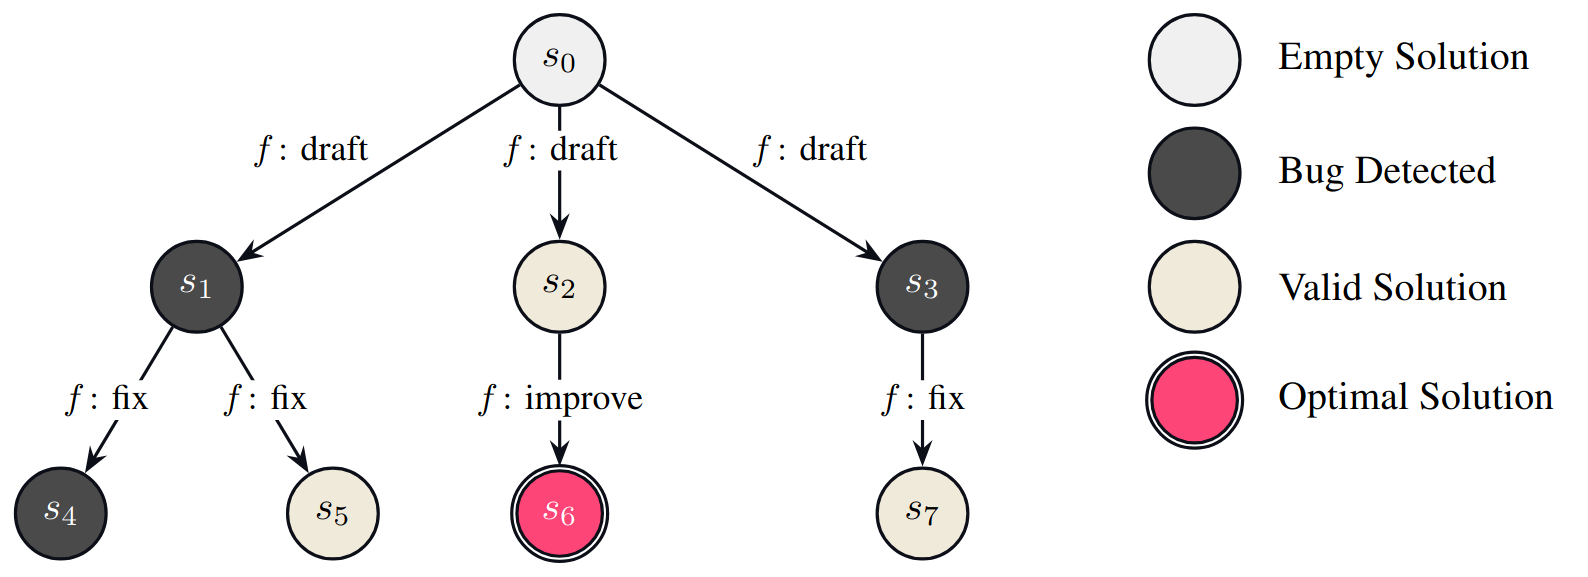
\includegraphics[width=0.8\linewidth]{images/aide-solution-tree.png}
%     \caption{A sample solution tree for AIDE, illustrating the drafting, fixing, and improvement steps. (Source: Schmidt et al., 2025, p. 4)}
%     \label{fig:enter-label}
% \end{figure}

% The Solution Tree ($T$): This is all discovered/proposed solutions (Python code scripts) and the improvement attempts (edges linking them) stored in a tree structure. The root solution ($s_0$) is typically an empty script, a node with value 'None'.

% Evaluator ($h$): This is a stateless function that takes a solution script as input and returns a scalar score (e.g., validation accuracy, loss). This score guides the search process. this evaluator is composed of a code interpreter that executes the code, then another LLM then takes the execution result (the trace back) and produces a structured output via function calling. this particular role is considered stateless since it always produce the same score, and it does not include past attempts in its evaluation, and this is important in the overall tree search for the best solution as every node or possible solution is evaluated primary on this.

% Search Policy ($\pi$): AIDE uses a simple, hard-coded search policy that determines the next step or next action. Based on the current state of the solution tree, it decides to:

% 1. Draft a new initial solution (if a desired number of diverse starting points hasn't been reached).

% 2. Debug a buggy node (if it's within a certain debug depth).

% 3. Improve an existing, non-buggy solution (typically targeting the current best-performing one).

% This policy has practical heuristics, such as initially exploring diverse solutions and then iteratively refining the most promising ones, while also limiting attempts to fix persistently broken solutions. Although this might be the most obvious area of improvement in the AIDE pipline, weather that was using a learned model that guides this search, the nature of the problems that small open source models have is largely not caused by the search heuristic, rather it is more fundamental in terms of ability to generate valid code in the first place, or correct usage of libraries and APIs.

% Coding Operator ($F$): This is the LLM itself as it proposes new scripts. It has three main entry points, each with specialized prompts:

% Drafting: Create a completely new solution `exploration`. The LLM is prompted to outline a plan to solve the problem (e.g., specify a neural network architecture and feature engineering ideas) and then generate a single-file Python program implementing that plan. These are then separated using regular expressions.

% Debugging: Repairing buggy solutions by inspecting error logs and execution traces. It attempts to fix issues like broken imports or incorrect tensor dimensions while preserving the overall approach.

% Improving: Called when a valid, non-buggy solution exists but could benefit from modifications (data preprocessing changes, architectural adjustments, or optimization tweaks and hiperparameter tuning). The LLM is prompted to propose a single `atomic` change, such as switching an optimizer or adding a regularization technique, so its impact on performance can be directly measured.

% Finally, to manage the LLM's context window and avoid `prompt explosion' from an  the growing history being fed to the model during the debugging and improvement phases, AIDE uses a summarization operator. Instead of appending all historical logs, this operator selectively extracts relevant information from the solution tree, such as Performance metrics (accuracy, AUC-ROC, etc.), Hyperparameter settings from previous attempts, Relevant hints for debugging (e.g., misaligned array shapes from trace-backs), This concise summary allows each code revision to be somewhat stateless yet guided by prior information, maintaining efficiency.

% Data Preview in Coding Prompts: AIDE also includes a small, static `data preview' in its coding prompts, providing the LLM with basic knowledge of the dataset's size or feature layout without needing extensive exploratory data analysis (EDA) at each step. As there is a code interpreter part of this iterative process, this Data preview tells the model exactly where and how the data is organized, and where to save its output or `submission.csv`

% The choice of AIDE as the foundational scaffold for this research is deliberate. It is open-source , it allows for the modification and integration of the inference-time scaling methods (self-consistency and self-reflection, etc) that are central to our work. Furthermore, AIDE's design, which explicitly models ML engineering as an iterative code optimization and tree search process powered by an LLM, provides a structured environment to study the effects of these techniques. It is established and proven to work effectively in solving ML tasks, as demonstrated in its original paper and subsequent evaluations on benchmarks like MLE-Bench, offers a great platform for experimentation. 

% AIDE has been tested and evaluated only using lagre-scale propriety LLMs, and our aim is to investigate how inference-time strategies can enhance AIDE's problem-solving capabilities, particularly its ability to make an open source, small-scale LLM generate more robust and higher-performing solutions on the challenging task like Machine learning Engineering.


% \section{MLE-Bench}
% To assess the performance of the enhanced aide scaffold we developed, we utilize the newly released MLE-bench, a benchmark for measuring how well AI agents perform at machine learning engineering, it is composed of 75 kaggle competitions, curated carefully from the Metakaggle dataset that contains around 5000 Kaggle competitions.
% This benchmark is designed specifically to be a benchmark for evaluating the performance of AI agents at machine learning engineering. MLE-Bench vary in category, scale, and complexity. This benchmark is designed not merely to test isolated skills, but to measure an agent's capacity for autonomous, end-to-end problem-solving—a workflow that spans model creation, training, evaluation, and iterative refinement.

% While MLE-Bench is a recent development, it is built upon a foundation of prior work aimed at evaluating LLMs coding and agentic abilities. Benchmarks like APPS (Hendrycks et al., 2021) and early evaluations of models such as Codex (Chen et al., 2021) have been used to measure general coding competence. The choice of MLE-Bench, and its particular relevance to this thesis, lies in its focus on tasks that are both representative of modern industry practices and known to be challenging for current AI systems, it offers a more specialized and demanding evaluation. However, it is very big benchmark, and evaluating on the 75 competitions is computationally infeasable for this thesis, hece, we opted for a subset of the benchmark,
% The core design of MLE-Bench is mostly around its task selection. The 75 selected competitions present an extremly difficult challenge for any coding agent. Essentially, MLE-Bench provides an offline Kaggle competition environment. For context, Kaggle is a platform that hosts data science and ML competitions where participants build predictive models to solve real-world challenges, competing for the best score on predefined metrics and earning rankings on a leaderboard. Top performers are often awarded monetary prizes, in addition to recognition with a bronze, silver, or gold medals. MLE-Bench adopts a similar structure to Kaggle, allowing for a realistic comparison of agent performance against historical human achievements 'offline leaderboard. The final results in this benchmark are often presented in terms of the average number of medals an agent would have won, determined by comparing its solution's metric on an unseen test set against the saved leaderboard from the original Kaggle competition.



% \section{Experiment Setup}

% To provide a rigorous and reliable evaluation of the inference-time strategies proposed in this thesis, a carefully designed experimental setup is essential. This section outlines the benchmark competitions, the baselines for comparison, the specific metrics used for evaluation, and the overall experimental procedure. The primary goal is to establish a solid evaluation framework that can take a given agent configuration as input and produce clear, quantitative metrics to determine its effectiveness relative to other methods.

% 1. Benchmark Competitions

% The foundation of our evaluation is a representative subset of competitions from the official MLE-Bench framework. While the full MLE-Bench is extensive, running experiments on all 75 competitions is computationally prohibitive for this project. Therefore, I have selected a curated subset of 10 competitions from the 'lite' complexity category. This choice was driven by several factors:

% Diversity: The selected competitions span 6 distinct machine learning categories, ensuring that our evaluation is not biased towards a single problem type. This diversity is crucial for assessing the general applicability of the proposed inference strategies.

% Feasibility: By focusing on 'lite' competitions, which are relatively lightweight in terms of data size and complexity, our experiments can focus on the quality of the agent's problem-solving process rather than being constrained by the technical overhead of handling massive datasets.

% Representativeness: This subset is a good representation of the full 'lite' category and provides a strong, empirical basis for evaluation.

% Flexibility: The chosen set is flexible enough to be extended in future work, either by including more competitions from the 'lite' category for a full standard comparison or by adding selected 'medium' complexity tasks to further test the limits of our methods.

% The 10 competitions selected for this benchmark are detailed in Table \ref{tab:competitions}.

% % \begin{table}[h!]
% % \centering
% % \caption{Selected Benchmark Competitions from MLE-Bench 'Lite' Category}
% % \label{tab:competitions}
% % \begin{tabular}{ll}
% % \hline
% % \textbf{Competition Name} & \textbf{Category} \ \hline
% % aerial-cactus-identification & Image Classification \
% % leaf-classification & Image Classification \
% % spooky-author-identification & Text Classification \
% % random-acts-of-pizza & Text Classification \
% % tabular-playground-series-may-2022 & Tabular \
% % nomad2018-predict-transparent-conductors & Tabular \
% % denoising-dirty-documents & Image to Image \
% % text-normalization-challenge-english-language & Sequence to Sequence \
% % text-normalization-challenge-russian-language & Sequence to Sequence \
% % mlsp-2013-birds & Audio Classification \ \hline
% % \end{tabular}
% % \end{table}

% 2. Baselines for Comparison

% To properly contextualize the performance of our proposed methods, we will benchmark them against a diverse set of established baselines. The aim is twofold: first, to prove that our strategies provide a meaningful improvement over a standard open-source model, and second, to demonstrate that these strategies make open-source models competitive with both closed-source counterparts and human experts.

% The baselines are summarized in Table \ref{tab:baselines}.

% % \begin{table}[h!]
% % \centering
% % \caption{Baselines for Performance Comparison}
% % \label{tab:baselines}
% % \begin{tabular}{lll}
% % \hline
% % \textbf{Baseline} & \textbf{Type} & \textbf{Reason for Inclusion} \ \hline
% % \textbf{AIDE + GPT-4o} & CS / High-Capability & Represents a strong, widely-used frontier model. \
% % & & Provides a high-water mark for performance. \ \
% % \textbf{AIDE + o4-mini} & CS / Reasoning-Optimized & Assumed to be a cost-effective, state-of-the-art reasoning \
% % & & model from OpenAI. Serves as a key SOTA reference. \ \
% % \textbf{AIDE + Llama 3.1 (405B)} & OS / High-Capability & A top-tier open-source model. Outperforming this \
% % & & demonstrates the power of our strategy. \ \
% % \textbf{Our Model + Default AIDE} & OS / Ablation & \textbf{Critical baseline.} This isolates the performance gain \
% % & & attributable specifically to our inference strategies, \
% % & & by removing them from our chosen model. \ \
% % \textbf{Human Performance} & Human Eval & Provides real-world context by comparing agent scores \
% % & & to the original Kaggle leaderboards. \ \hline
% % \end{tabular}
% % \end{table}

% 3. Evaluation Metrics

% To capture a holistic view of agent performance, we will use a suite of metrics inspired directly by the MLE-Bench and AIDE papers. These metrics evaluate an agent's ability to produce functional code, understand the task requirements, and ultimately generate an optimal solution.

% Code and Submission Generation: These metrics assess the fundamental ability of the agent to generate working code and complete the task.

% Valid Code Rate (\%): The number of steps that produce a valid, executable script divided by the total number of steps, averaged across seeds and competitions. A higher rate indicates a stronger fundamental code generation capability.

% Valid Submission Rate (\%): The percentage of independent runs (i.e., per seed, per competition) that successfully produce a submission file that passes the benchmark's validity checks. This is a stricter measure of task completion.

% Performance Against Human Baselines: Once a valid submission is produced, its quality is scored against the historical human leaderboard.

% Above Median (\%): The percentage of competitions where the agent's best score is strictly better than the median score achieved by human participants.

% Any Medal (\%): The percentage of competitions where the agent's best score is high enough to have earned a bronze, silver, or gold medal according to official Kaggle rules. This is our headline metric for overall success.

% The final results for each agent configuration will be presented in a summary table, as shown in the template in Table \ref{tab:results_template}.

% % \begin{table}[h!]
% % \centering
% % \caption{Template for Aggregated Results Table}
% % \label{tab:results_template}
% % \begin{tabular}{lccc}
% % \hline
% % \textbf{Model + Method} & \textbf{Valid Submission (\%)} & \textbf{Above Median (\%)} & \textbf{Any Medal (\%)} \ \hline
% % AIDE + o4-mini & X% 
% % ±
% % ±
% %  Y & X% 
% % ±
% % ±
% %  Y & X% 
% % ±
% % ±
% %  Y \
% % Our Model + Strategy 1 & X% 
% % ±
% % ±
% %  Y & X% 
% % ±
% % ±
% %  Y & X% 
% % ±
% % ±
% %  Y \
% % Our Model + Default AIDE & X% 
% % ±
% % ±
% %  Y & X% 
% % ±
% % ±
% %  Y & X% 
% % ±
% % ±
% %  Y \ \hline
% % \end{tabular}
% % \end{table}

% 4. Experimental Procedure

% To ensure a fair and repeatable evaluation, all experiments are conducted using a standardized protocol within a consistent environment.

% Environment: All runs are executed within a Dockerized environment to ensure consistency. AIDE is configured with fixed hyperparameters for all methods (e.g., 20 steps per attempt, 5 initial drafts).

% Execution: For each of the 10 competitions, every agent configuration ("Method") is run for k=3 independent attempts (seeds). This helps account for the inherent stochasticity of LLMs.

% Data Collection: After each run, we automatically collect the raw data, including whether a valid submission was generated and its corresponding score.

% Metric Calculation: Using the collected data, we calculate the flags for Valid Submission, Above Median, and Any Medal for each run.

% Aggregation: These flags are then aggregated. For metrics like Above Median and Any Medal, we consider a competition "solved" if at least one of the three seeds was successful (a pass@3 approach). The final percentages are averaged across the 10 competitions, with results reported as mean ± standard error.

% This standardized pipeline ensures that as we introduce and test new inference-time strategies, the results are directly and fairly comparable to our established baselines.



% % This is essentially what AIDE’s “solution tree” does conceptually – it navigates a solution space tree by proposing variations and seeing which yields better scores. Another formulation is the Tree-of-Thoughts
% % approach (Yao et al., 2023) where the model can propose multiple thoughts (steps of a solution)

% % This is somewhat what AIDE does by default (running the full training code to get a score), but one could go further and allow fine-grained tool use: the agent could execute just a part of the code (say a data pre-processing step) to inspect intermediate results, or call a library function to check documentation, etc. Another tool is a web browser or documentation fetcher, useful if the coding problem needs external knowledge
% % (though MLE-bench specifically disallows internet to prevent cheating). Still, 

% % For instance, in
% % OpenAI’s tests, they tried different “scaffolds”: AIDE, ResearchAgent, CodeAct, etc., each of which
% % structures the LLM’s process differently. 

% % AIDE’s self-reflection is essentially
% % an internal critic role given to the same model. We could also have a different model entirely
% % serve as the critic – for instance, use a 13B model to generate code and a more reliable 13B or
% % a set of heuristic rules to review it. This two-model system was not explicitly used in AIDE (to
% % our knowledge, AIDE uses one model for everything), but it’s a viable ITS approach: compose
% % multiple smaller experts rather than rely on one monolith. Each expert at inference time does
% % part of the task. 

% % search algorithms to explore solution space, tool use to gain information or verify outputs during generation, and modular agent frameworks that break the task into
% % pieces handled sequentially. These methods have proven effective: for example, using a Process Reward
% % Model + search enabled a 3B model to outperform a 70B model on a math benchmark, and
% % self-debugging allowed models to fix errors that they would otherwise miss. Importantly, most of these
% % techniques do not require fine-tuning the base model – they work by manipulating the inference
% % process (through prompting, iterating, or orchestration). Some advanced methods do introduce learned
% % components (e.g. training a verifier network, or fine-tuning the model to better utilize reflections), which blurs the line between pure inference-time and training. We’ll discuss a few such cases as well, but
% % the primary focus is on what can be done on the fly with an off-the-shelf model. The ultimate goal of
% % 5these strategies is well captured by OpenAI’s notion of “self-verification”, where the model can reliably
% % check its own work instead of relying on a giant ensemble or an external judge. In the next section,
% % we propose concrete techniques from these categories that AIDE could adopt to further empower its
% % small-model code generation in the ML domain.
% % **EITHER SPEAK ABOUT AIDE AND MLE BENCH HERE OR IN THE METHODS SECTINO** % You do not need to have exactly 4 chapters.
%                  % It is probably a good minimum, with 5 chapters 
%                  % average, and 7 chapters might be a maximum.
% % \chapter{Summary of Results}

% This chapter provides a concise overview of the experimental results, presenting the key aggregate performance metrics and empirical code generation capabilities for the evaluated agent configurations on the MLE-Bench subset.

% \section{Aggregate Performance Summary}

% Table \ref{tab:summary_aggregate} summarizes the overall performance of each model configuration, focusing on key metrics such as Valid Submission Rate (VSR), Above Median Rate (AMR), and Any Medal Rate (Pass@3). Made Submission is also included as a primary pipeline success indicator.

% \begin{table}[h!]
%     \centering
%     \caption{Summary of Aggregate Performance Metrics}
%     \label{tab:summary_aggregate}
%     % Using tabularx to make the table fit within the text width
%     \begin{tabularx}{\textwidth}{p{4.5cm} *{4}{>{\centering\arraybackslash}X}}
%         \toprule
%         Method                      & Made Submission (\%) & Valid Submission (\%) & Above Median (\%) & Any Medal (Pass@3 \%) \\
%         \midrule
%         \textbf{AIDE} & & & & \\
%         AIDE + o1-preview          & - & - & - & - \\
%         AIDE + GPT-4-turbo         & 73.3 $\pm$ 3.3 & 63.3 $\pm$ 3.3 & 20.0 $\pm$ 5.8 & 6.7 \\ % Pass@3 based on provided table
%         AIDE + gpt-4o-mini         & 76.7 $\pm$ 2.4 & 63.3 $\pm$ 2.4 & 26.7 $\pm$ 2.4 & 10.0 \\ % Pass@3 based on provided table
%         AIDE + DeepSeek-7B (Base)  & 23.3 $\pm$ 3.3 & 20.0 $\pm$ 0.0 & 0.0 $\pm$ 0.0 & 0.0 \\ % Pass@3 based on provided table
%         AIDE + DeepSeek-7B + SR    & - & - & - & - \\
%         AIDE + DeepSeek-14B (Base) & 73.3 $\pm$ 2.4 & 60.0 $\pm$ 4.1 & 10.0 $\pm$ 4.1 & 10.0 \\ % Pass@3 based on provided table
%         AIDE + DeepSeek-14B + SR   & - & - & - & - \\
%         AIDE + DeepSeek-32B (Base) & 76.7 $\pm$ 3.3 & 63.3 $\pm$ 3.3 & 33.3 $\pm$ 3.3 & 20.0 \\ % Pass@3 based on provided table
%         AIDE + DeepSeek-32B + SR   & - & - & - & - \\
%         \midrule
%         \textbf{Human Performance} & - & - & 50.0 & 12.4 \\
%         \bottomrule
%     \end{tabularx}
%     \caption*{\textbf{Note}: Metrics are mean $\pm$ standard error of the mean, averaged across 10 competitions and 3 seeds, except for Pass@3 which is the percentage of competitions with at least one medal across 3 seeds. SR denotes Self-Reflection strategy. Entries marked '-' indicate data was not available in the provided context.}
% \end{table}

% \section{Empirical Code Generation and Submission Attempt Summary}

% Table \ref{tab:summary_empirical} provides a summary of the average empirical metrics, highlighting the agent's code generation capabilities and pipeline progression based on Valid Code Generation Rate (VCGR), CSV Submission Attempt Rate (CSAR), Average Steps to First Working Output (StepsToWO), and Average Code Quality.

% \begin{table}[h!]
%     \centering
%     \caption{Summary of Empirical Code Generation and Submission Attempt Metrics}
%     \label{tab:summary_empirical}
%     % Using tabularx to make the table fit within the text width
%     \begin{tabularx}{\textwidth}{p{4.5cm} *{5}{>{\centering\arraybackslash}X}}
%         \toprule
%         Metric                     & AIDE + gpt-4o-mini & AIDE + GPT-4-turbo & AIDE + DeepSeek-7B (Base) & AIDE + DeepSeek-14B (Base) & AIDE + DeepSeek-32B (Base) \\
%         \midrule
%         VCGR (\%)                   & 40.53              & 40.40              & 3.73                      & 24.83                      & 25.63                      \\
%         CSAR (\%)                   & 41.47              & 41.87              & 4.93                      & 29.24                      & 26.50                      \\
%         Avg. Steps to First WO     & 9.77               & 12.00              & 28.77                     & 13.86                      & 13.56                      \\
%         Avg. Code Quality (1-10)    & 5.76               & 5.86               & 3.66                      & 5.00                       & 5.26                       \\
%         \bottomrule
%     \end{tabularx}
%     \caption*{\textbf{Note}: Metrics are averaged over all available runs (typically 10 competitions $\times$ 3 seeds). VCGR is the percentage of steps generating valid code. CSAR is the percentage of steps attempting a CSV submission. StepsToWO is the average number of steps to the first working output (using the \texttt{StepsToWO\_inf\_replaced} value from the source data). Avg. Code Quality is on a scale of 1--10. Data for models with the Self-Reflection strategy was not available in the provided aggregate empirical summaries.}
% \end{table} % Conclusion is usually a chapter itself. 
% %\chapter{Discussion and Conclusion}

This chapter provides a concise overview of the experimental results, presenting the key aggregate performance metrics and empirical code generation capabilities for the evaluated agent configurations on the MLE-Bench subset.

\section{Aggregate Performance Summary}

Table \ref{tab:summary_aggregate} summarizes the overall performance of each model configuration, focusing on key metrics such as Valid Submission Rate (VSR), Above Median Rate (AMR), and Any Medal Rate (Pass@3). Made Submission is also included as a primary pipeline success indicator.

\begin{table}[h!]
    \centering
    \caption{Summary of Aggregate Performance Metrics}
    \label{tab:summary_aggregate}
    % Using tabularx to make the table fit within the text width
    \begin{tabularx}{\textwidth}{p{4.5cm} *{4}{>{\centering\arraybackslash}X}}
        \toprule
        Method                      & Made Submission (\%) & Valid Submission (\%) & Above Median (\%) & Any Medal (Pass@3 \%) \\
        \midrule
        \textbf{AIDE} & & & & \\
        AIDE + o1-preview          & - & - & - & - \\
        AIDE + GPT-4-turbo         & 73.3 $\pm$ 3.3 & 63.3 $\pm$ 3.3 & 20.0 $\pm$ 5.8 & 6.7 \\ % Pass@3 based on provided table
        AIDE + gpt-4o-mini         & 76.7 $\pm$ 2.4 & 63.3 $\pm$ 2.4 & 26.7 $\pm$ 2.4 & 10.0 \\ % Pass@3 based on provided table
        AIDE + DeepSeek-7B (Base)  & 23.3 $\pm$ 3.3 & 20.0 $\pm$ 0.0 & 0.0 $\pm$ 0.0 & 0.0 \\ % Pass@3 based on provided table
        AIDE + DeepSeek-7B + SR    & - & - & - & - \\
        AIDE + DeepSeek-14B (Base) & 73.3 $\pm$ 2.4 & 60.0 $\pm$ 4.1 & 10.0 $\pm$ 4.1 & 10.0 \\ % Pass@3 based on provided table
        AIDE + DeepSeek-14B + SR   & - & - & - & - \\
        AIDE + DeepSeek-32B (Base) & 76.7 $\pm$ 3.3 & 63.3 $\pm$ 3.3 & 33.3 $\pm$ 3.3 & 20.0 \\ % Pass@3 based on provided table
        AIDE + DeepSeek-32B + SR   & - & - & - & - \\
        \midrule
        \textbf{Human Performance} & - & - & 50.0 & 12.4 \\
        \bottomrule
    \end{tabularx}
    \caption*{\textbf{Note}: Metrics are mean $\pm$ standard error of the mean, averaged across 10 competitions and 3 seeds, except for Pass@3 which is the percentage of competitions with at least one medal across 3 seeds. SR denotes Self-Reflection strategy. Entries marked '-' indicate data was not available in the provided context.}
\end{table}

% \section{Empirical Code Generation and Submission Attempt Summary}

% Table \ref{tab:summary_empirical} provides a summary of the average empirical metrics, highlighting the agent's code generation capabilities and pipeline progression based on Valid Code Generation Rate (VCGR), CSV Submission Attempt Rate (CSAR), Average Steps to First Working Output (StepsToWO), and Average Code Quality.

% \begin{table}[h!]
%     \centering
%     \caption{Summary of Empirical Code Generation and Submission Attempt Metrics}
%     \label{tab:summary_empirical}
%     % Using tabularx to make the table fit within the text width
%     \begin{tabularx}{\textwidth}{p{4.5cm} *{5}{>{\centering\arraybackslash}X}}
%         \toprule
%         Metric                     & AIDE + gpt-4o-mini & AIDE + GPT-4-turbo & AIDE + DeepSeek-7B (Base) & AIDE + DeepSeek-14B (Base) & AIDE + DeepSeek-32B (Base) \\
%         \midrule
%         VCGR (\%)                   & 40.53              & 40.40              & 3.73                      & 24.83                      & 25.63                      \\
%         CSAR (\%)                   & 41.47              & 41.87              & 4.93                      & 29.24                      & 26.50                      \\
%         Avg. Steps to First WO     & 9.77               & 12.00              & 28.77                     & 13.86                      & 13.56                      \\
%         Avg. Code Quality (1-10)    & 5.76               & 5.86               & 3.66                      & 5.00                       & 5.26                       \\
%         \bottomrule
%     \end{tabularx}
%     \caption*{\textbf{Note}: Metrics are averaged over all available runs (typically 10 competitions $\times$ 3 seeds). VCGR is the percentage of steps generating valid code. CSAR is the percentage of steps attempting a CSV submission. StepsToWO is the average number of steps to the first working output (using the \texttt{StepsToWO\_inf\_replaced} value from the source data). Avg. Code Quality is on a scale of 1--10. Data for models with the Self-Reflection strategy was not available in the provided aggregate empirical summaries.}
% \end{table} % You may have more chapters. (Use e.g. git add FILE)
% % This is where we stop counting pages.
% % Acknowledgements and References are not counted.
% %-----------------------------------------------------------------------------
% % See the acknowledgement.tex file and follow the instructions there.
% \chapter*{Acknowledgements}
% Don't change anything above this.
% We do not number this or add it to the contents!
% Overly long acknowledgements are not professional.

I want to acknowledge AIMS and it's funders for supporting this work, as well as my supervisor, Prof Arnu Pretorius from University of Stellenbosch, and my co-supervisor, Arnol Fokam from InstaDeep.

I would also like to thank my family and friends, and my colleagues at AIMS for their support and encouragement.

% %-----------------------------------------------------------------------------
% % Note the errata page is not for now, it is for use during the examination.
% % Not that you're going to have any errata.
% %-----------------------------------------------------------------------------
% % THE BIBLIOGRAPHY 
% % Bibliography styles define how the bibliography is 
% % listed and formatted. This is part of the AIMS house
% % style and is only changed under exceptional circumstances
% \renewcommand{\bibname}{References}
% \nocite{*}
% \bibliographystyle{myabbrvnat}
% \bibliography{references}
% \addcontentsline{toc}{chapter}{References}
% %-----------------------------------------------------------------------------
% \end{document}



% \end{RLtext}\\
% \vfill
% \section*{Declaration}
% I, the undersigned, hereby declare that the work contained in this research project is my original work, and that any work done by others or by myself previously has been acknowledged and referenced accordingly.

% % \includegraphics[height=2cm]{images/signature.png} \newline \hrule
% Asim Osman, 12 May 2025


% A short, abstracted description of your research project goes here. 
% It should be about 100 words long. But write it last.

% An abstract is not a summary of your research project: it's an abstraction of that. 
% It tells the readers why they should be interested in your research project but summarises all
% they need to know if they read no further.

% The writing style used in an abstract is like the style used in the rest of your research project: concise, clear and direct. 
% In the rest of the research project, however, you will introduce and use technical terms. In the abstract you should
% avoid them in order to make the result comprehensible to all.

% You may like to repeat the abstract in your mother tongue.

% At a unviersity like Stellenbosch you *must* produce an abstract in Afrikaans for your masters.
% At AIMS you are encouraged to repeat the abstract in your mother tongue
% French, Igbo, Mlagasy, etc. just write it using LaTeX's special
% characters.
% Arabic students see the arabic.tex file for an example
% Amharic use openoffice and export from there and import a figure here.
% Where the words do not exist put the English work in italics, or use mathematical symbols.



% Do not change anything below this except for adding your
% signature (replace images/signature.png) and your name.


--------------------------------------------------------------------------
% % Template for AIMS Structured Masters Research Project
% %
% % The fonts, linespacing, numbering, page styles, order
% % of  Title/Abstract/TOC/Body/{Appendices}/Acknowledgements/References 
% % are prescribed as the AIMS house style.
% %
% % Do not change them or add to it without getting approval first.
% % Essays are not accepted if they do not follow house style.
% % This is in preparation for your Masters where the university
% % will be much more strict on the house style.
% %
% \documentclass{aimsessay}
% % \usepackage{etex} % fix for using xy and tikz in the same document
% \usepackage[utf8]{inputenc}
% \usepackage[T1]{fontenc}
% \usepackage{lmodern}
% \usepackage[round]{natbib}
% \usepackage{amsmath}
% \usepackage{amsfonts}
% \usepackage{amssymb}
% \usepackage{mathtools}
% \usepackage{latexsym}
% \usepackage{parskip}
% \usepackage{enumerate}
% \usepackage{tikz}
% \usepackage{lipsum}
% % Fix spacing before theorem environments
% \makeatletter\def\thm@space@setup{%
%   \thm@preskip=1.2\parskip \thm@postskip=0pt
%   }
% %\makeatother
% % Reduce space before proof
% %\makeatletter
% \renewenvironment{proof}[1][\proofname]{\par
%   \vspace{-\topsep}% remove the space after the theorem
%   \pushQED{\qed}%
%   \normalfont
%   \topsep0pt \partopsep0pt % no space before
%   \trivlist
%   \item[\hskip\labelsep
%         \itshape
%     #1\@addpunct{.}]\ignorespaces
% }{%
%   \popQED\endtrivlist\@endpefalse
%   \addvspace{6pt plus 6pt} % some space after
% }
% \makeatother
% % Reduce spacing around section headings?
% %
% %-----------------------------------------------------------------------------
% % To use external packages for specific needs, 
% % get approval before adding them here (they
% % should not override general AIMS house style and layout).
% %
% % Examples:
% % 
% % Load caption before arabtex
% \usepackage{caption} %many figures in one figure (note subfigure and subfig are deprecated) 
% \usepackage{subcaption} %many figures in one figure (note subfigure and subfig are deprecated) 
% % For Arabic
% %\usepackage{arabtex}
% %\usepackage{utf8}
% %\setcode{utf8}
% % For tables:
% \usepackage{booktabs} % \toprule, \midrule, \bottomrule
% \usepackage{array}    % \newcolumntype
% % 
% % For figures:
% %\usepackage[below,section]{placeins} % use \FloatBarrier in the body to really force a float somewhere. Please limit use.
% \usepackage{float}  %"H" placement spec, for **really here** (i.e. not float)
% %
% % For code and algorithms
% \usepackage{moreverb}   % \verbatimtabinput
% % \usepackage{listings} % more flexible and complicated 
%                         % than moreverb and algorithm
% % 
% % Others
% % \usepackage[all]{xy}  %  if you use this uncomment \usepackage{etex} above to fix a conflict with tikz.
% % \usepackage{sagetex}
% % \usepackage{siunitx} % to typeset numbers, units, align decimals in tables.
% % \usepackage{dcolumn} % less flexible but maybe faster than siunitx above.
% % \usepackage{mathtools} % More maths, e.g. \mathclap.
% %
% % Others may be landscape, longtable, algorithm, algorithmic, etc.
% % 
% % ----------------------------------------------------------------------------
% % An AIMS Essay can use the sectioning commands "\chapter", "\section",
% % "\subsection". No "\subsubsection", "\paragraph", etc. They are disabled.
% % 
% % For Theorems and such, use the environments defined here:
% % \begin{thm}...\end{thm} (or "lem", "defn", etc)
% % 
% % We put the number to the left of the Theorem heading.
% \swapnumbers 
% % 
% % Theorems are in italics.
% \theoremstyle{plain}
% \newtheorem{thm}[subsection]{Theorem}
% %
% % Rest is not in italics.
% \theoremstyle{definition} 
% \newtheorem{lem}[subsection]{Lemma}
% \newtheorem{cor}[subsection]{Corollary}
% \newtheorem{conj}[subsection]{Conjecture}
% \newtheorem{pro}[subsection]{Proposition}
% \newtheorem{exa}[subsection]{Example}
% \newtheorem{defn}[subsection]{Definition}
% \newtheorem{rem}[subsection]{Remark}
% % 
% % If you have no theorems, but a lot of equations, maybe the
% % following two lines are good. Beware of corresponding Equation
% % and Example numbers though! Number equations by sections.
% % 
% \numberwithin{equation}{section}
% %
% %-----------------------------------------------------------------------------
% % Abstracts are usually written in English, with a version in your
% % mother tongue underneath.
% %
% % French, Igbo, Malagasy, etc. students use normal LaTeX
% % for special characters, for example \'{e}
% %
% % Amharic students use LibreOffice to write Amharic,
% % export and include a figure.
% %
% %\begin{RLtext}    
% %Here is where the arabic text goes.
% %You can just type it with an arabic keyboard
% %\end{RLtext}\\
% %-----------------------------------------------------------------------------
 
% % Your own command shortcuts can go here
% % keep them clearly separate from other sections of the preamble
% % It is good style to have only a few of these so that
% % we can read one another's code. If you have to many, 
% % then your code does not compile in someone else's template easily,
% % and it makes it harder to read. These definitions are only
% % meant for very often-used commands to save typing; Examples:
% %
% %\newcommand {\be}{\begin{equation}}
% %\newcommand {\ee}{\end{equation}}
% %\newcommand {\C}{\mathbb{C}} % Complex
% %\newcommand {\Z}{\mathbb{Z}} % Integers
% %\newcommand {\R}{\mathbb{R}} % Real
% %\DeclareMathOperator{\sech}{sech} % declaring new math operators like \sin.
% %  
% %-----------------------------------------------------------------------------
% % Title & Author
% % On this page you must have NO full-word capitalizations, bold, or colour. 
% % All AIMS research projects per year have the same title page.
% % In English your family name is written last, i.e. Firstname LASTNAME
% % English Capitalization, not as in some Francophone countries where
% % you write LASTNAME, Firstname.
% % Put your AIMS email address only please, for consistency,
% % not gmail or some other webmail address.
% \title{The Essay Title goes here Rafa\l Rafa\L{} test}
% % Your name must be in English Capitalisation with no comma, 
% % and the Family name comes last.
% \author{Firstname Middlename Familyname (email@aims.ac.za)\\
% % Then in the MAIN BODY use this:                  
% %\begin{RLtext}
% %نووووووسسسسح
% %\end{RLtext}\\
% %%%%%%%%%%%%%%%%%%%%%%%%%%%%%%%%%%%
% %\begin{otherlanguage}{arabtext}
% %شةشىغ
% %\end{otherlanguage}\\
% %%%%%%%%%%%%%%%%%%%%%%%%%%%%%%%%%%%%%
% % Amharic students speak to me about how to add your name in your own alphabet.
% % Everything here is prescribed; do not enter bold or ALL CAPS here,
% % it will not be accepted.
% African Institute for Mathematical Sciences (AIMS)\\
% \\
% % Example1
% {\small Supervised by: Title Firstname Lastname}\\
% {\small Institute of Supervisor, Country}%\\
% % For second/more supervisors, continue with another line, e.g.
% % {\small and Dr So And-so}
% % {\small University of Life, Country}
% % Don't put the department, it becomes too long.
% }
% \date{{\small 24 October 2024}\\%
%   {\scriptsize\it Submitted in partial fulfillment of 
%     a structured masters degree at AIMS South Africa}\\%
%   \vspace{0.5cm}{\includegraphics{images/AIMS_SA_Logo.pdf}}}
% %-------------------------------------------------------------------------
% \begin{document}
% %\selectlanguage{english}
% \pagestyle{empty}
% \maketitle
% % All other files are included via \input. 
% % To compile in texmaker while viewing any of those
% % without having to switch back, use
% %   Options > Define Current Document as 'Master Document'
% % To not have to close a PDF, remove viewpdf from quickbuild 
% % and open the PDF (once) manually: it will auto-refresh or with control-r
% % 
% %-------------------------------------------------------------------------
% % The abstract is the first thing we want to see. No acknowledgements or 
% % dedications here. Fetch the abstract from a separate file.
% % Please write it in English and in your mother tongue.
% % An abstract should be less than half a page, so that both abstracts 
% % (that is both languages) fit onto one page.
% % We number roman numerals until the main body
% \pagenumbering{roman}
% \chapter*{Abstract}
\addcontentsline{toc}{chapter}{Abstract}
Recent findings suggest that reasoning strategies applied during inference can yield more significant performance gains in large language models (LLMs) than merely increasing their parameter scale. Furthermore, the emergence of advanced open-source LLMs, such as those distilled from DeepSeek-R1—which matches the performance of its closed-source counterpart, OpenAI-o1, offers new opportunities for exploration. Leveraging these more capable LLMs, we aim to evaluate their performance on complex tasks in machine learning engineering.

To this end, MLE-Bench provides an ideal benchmark. Designed to assess the machine learning engineering capabilities of AI agents, MLE-Bench comprises 75 diverse Kaggle competitions. Its primary goal is to comprehensively evaluate AI agents' ability to design and implement end-to-end machine learning pipelines, making it a rigorous testbed for these advanced LLMs.

This project examines the effectiveness of these distilled open-source LLMs when paired with inference-time reasoning strategies within and Agentic framework, on the machine learning tasks presented by MLE-Bench. The primary objective is to compare the performance of these open-source models with the more established LLM-based approaches outlined in the MLE-Bench paper. Ultimately, this work supports the broader vision of integrating LLM-based agentic systems into AI research workflows.

% \begin{otherlanguage}{arabic}
%     هذا هو الملخص العربي لمشروع البحث الخاص بك.
% \end{otherlanguage}
\vfill

\section*{Declaration}

I, the undersigned, hereby declare that the work contained in this research project is my original work, and that any work done by others or by myself previously has been acknowledged and referenced accordingly.
% \includegraphics[height=2cm]{images/signature.png} \newline \hrule

Asim Osman, 12 June 2025
% % Don't go typing out the contents.
% \tableofcontents
% \newpage
% % We switch to arabic numerals here where your page count starts
% % Essays must be close to 30 pages long *starting here* and up to and including
% % the conclcusion. It does not include the acknowledgements or references.
% % 
% % Figures may differ between topics, but they are not there
% % to fill the pages -- they must add meaning.
% % In general most figures should be 0.8 times the width of the page
% % (perhaps wider in total when two or three columns of figures)
% % See the example in chapter one for defining that. Be *consistent*
% % in your presentation of information.
% \pagenumbering{arabic}
% \pagestyle{myheadings}
% %-----------------------------------------------------------------------------
% % Each chapter goes in a separate file
% % Chapter titles are just examples
% % Always have a question
% % Note the Case Pattern used at AIMS
% \chapter{Introduction}

Over the last few years, advancements in large language models have primarily relied on scaling up the number of parameters alongside increasing dataset size and compute budgets. This strategy, often referred to as train-time compute scaling, has been remarkably effective, significantly and consistently improving model performance on tasks such as translation, general question answering, and sophisticated reasoning in mathematics and coding. However, the exponential growth in model size and the associated costs have become prohibitively expensive, pushing training budgets to the billion-dollar scale and raising concerns about resource sustainability, particularly as high-quality training data becomes scarcer.

Consequently, significant interest has shifted toward inference-time (or test-time) scaling techniques. Rather than focusing on costly retraining and larger models, inference-time scaling enhances existing models by dedicating additional computational resources during prediction. These methods enable models to "think longer" on challenging problems by dynamically generating multiple reasoning paths, employing voting mechanisms, or iteratively refining their outputs. Recent studies, such as DeepMind's compute-optimal scaling \citep{placeholder}, demonstrate how smaller models can achieve impressive performance through adaptive inference strategies, sometimes even outperforming substantially larger models.

In parallel with these developments, there has been a notable emergence of "reasoning" or "thinking" models, designed explicitly to enhance models' capabilities to reason through complex problems. A prime example is DeepSeek-R1, which explicitly trains models using reinforcement learning to produce long, structured chains of thought before providing an answer, enabling LLMs to systematically tackle tasks that were previously challenging even for large-scale models. DeepSeek released a series of small distilled models trained on reasoning datasets generated from the original R1 model, empowering them with remarkable reasoning capabilities and improving their performance relative to larger models.

Motivated by these developments, this work explores the promise of inference-time scaling techniques applied to small-scale language models-particularly those distilled from DeepSeek-that are specifically designed for coding and machine learning engineering tasks, areas still challenging even for frontier models. Smaller models have substantial advantages in accessibility, rapid deployment, and lower operational costs, but traditionally lack the advanced reasoning capabilities exhibited by larger models. Through systematic implementation and evaluation of strategies such as chain-of-thought prompting, iterative self-refinement, self-consistency, and other methods, this project aims to bridge the performance gap. Ultimately, this thesis evaluates the extent to which inference-time scaling can address complex tasks such as machine learning engineering. We demonstrate that, with carefully designed inference-time enhancements, small-scale models can significantly improve performance in complex coding and engineering contexts, presenting a viable and cost-effective alternative to training massive foundational models.

% \section{Introduction}
% The field of artificial intelligence is witnessing an unprecedented scaling race, where models with hundreds of billions of parameters demonstrate remarkable capabilities that seem to emerge from sheer computational scale. This phenomenon has created a stark divide in the AI landscape: while large proprietary models like GPT-4 and Claude achieve impressive performance on complex reasoning and coding tasks, smaller open-source alternatives lag significantly behind, creating substantial barriers to accessibility and democratization of AI capabilities.
% This performance gap is particularly pronounced in machine learning engineering tasks, where AI agents must not only write syntactically correct code but also reason about complex architectural decisions, debug intricate workflows, and navigate the nuanced requirements of end-to-end ML pipelines. Unlike general-purpose coding, ML engineering demands sophisticated reasoning about data preprocessing, model selection, hyperparameter optimization, and deployment considerations—capabilities that have remained largely the domain of expensive, proprietary models.
% The emergence of inference-time scaling (ITS) techniques offers a promising pathway to bridge this performance divide. Rather than requiring massive computational resources during training, ITS methods like chain-of-thought prompting, self-consistency, and iterative refinement allow smaller models to achieve enhanced performance by investing additional computation during inference. This paradigm shift suggests that the reasoning capabilities necessary for complex tasks might be accessible to open-source models through strategic application of ITS techniques.
% Recent advances in distilled reasoning models, particularly DeepSeek-R1's family of models ranging from 7B to 32B parameters, present an opportunity to test this hypothesis. These models demonstrate strong reasoning capabilities even at smaller scales, potentially providing the foundation needed for effective ML engineering agents when enhanced with appropriate ITS strategies.
% However, existing agentic frameworks have primarily focused on proprietary models accessed through APIs, leaving open-source implementations under-explored. While ITS techniques have been applied to coding tasks, their systematic integration with distilled reasoning models specifically for ML engineering remains largely uncharted territory. This gap represents both a technical opportunity and a practical necessity for organizations seeking to develop their own AI assistants without relying on expensive proprietary solutions.
% This thesis addresses these challenges by developing and evaluating an enhanced version of AIDE (AI-Driven Exploration), an open-source agentic scaffold specifically tailored for inference-time scaling with open-source models. Our approach integrates multiple ITS strategies—including self-consistency, iterative self-debugging, and modular task decomposition—with DeepSeek-R1 distilled models to create accessible ML engineering agents capable of autonomously tackling complex machine learning competitions.
% Contributions
% This work makes four key contributions to the field:

% High-Performance Open-Source Infrastructure: We develop a high-throughput parallel inference engine with multiprocess orchestration, enabling simultaneous experimentation across different models and tasks while maintaining competitive inference speeds for open-source deployments.
% Specialized Agentic Scaffold: We create an open-source agent framework specifically designed for the HuggingFace ecosystem, providing an alternative to proprietary API-based solutions and enabling broader accessibility to ML engineering automation.
% Systematic ITS Integration: We implement and evaluate multiple variants of AIDE, each incorporating different ITS strategies, providing a comprehensive exploration of inference-time scaling techniques for ML engineering tasks. These variants are made available as separate repository branches with a unified interface for strategy selection.
% Empirical Validation: We demonstrate that a 32B open-source model enhanced with appropriate ITS techniques can achieve performance comparable to GPT-4 Turbo on ML engineering tasks, reaching a practical level where the agent can autonomously solve Kaggle competitions end-to-end.

% Thesis Overview
% The remainder of this thesis is organized as follows. Chapter 2 provides essential background on agentic systems in research workflows, reviews the effectiveness of ITS techniques across domains, introduces the concept of agent scaffolding, and surveys existing benchmarks for evaluating ML engineering capabilities. Chapter 3 details our methodology, including the original AIDE framework, MLE-Bench evaluation protocols, and our systematic approach to integrating ITS strategies within the agentic scaffold. We discuss experimental design choices, cost considerations, baseline selection rationale, and provide detailed implementation insights for each ITS method. Chapter 4 presents comprehensive experimental results, including numerical evaluations of agent performance, analysis of observed behaviors, and discussion of failed approaches. Finally, Chapter 5 concludes with implications for future research and practical deployment considerations.
% Through this systematic investigation, we aim to demonstrate that the performance gap between proprietary and open-source models in ML engineering can be substantially reduced through careful application of inference-time scaling techniques, opening new avenues for accessible and democratized AI-driven automation in machine learning workflows. % Introduction is usually a chapter itself.
% \chapter{Background and Related Work}

\section{Background}

\subsection{Large Language Models (LLMs)}
Large Language Models (LLMs) are neural networks trained on extensive text datasets, capable of generating human-like text. Based primarily on the transformer architecture, these models utilize a straightforward predictive objective, leveraging enormous volumes of data to tackle complex problems and diverse natural language tasks [CITATION], including translation [CITATION], semantic analysis [CITATION], and information retrieval.

Recent advancements in LLMs, exemplified by models such as the GPT series [CITATION*3] and the Llama family [CITATION], have been driven by significant scale, reaching billions of parameters. This substantial scale has unlocked emergent abilities—advanced skills like reasoning and in-context learning—that smaller models typically do not exhibit. These emergent capabilities enable LLMs to solve arithmetic problems, answer intricate questions, and summarize complex passages, often without explicit task-specific training.

\subsection{Scaling Laws and Train-Time Compute}
Scaling lows shows how the performance of Large Language models improves in a predeictable way with the increase in the parameter size, training data and computationa; resources, openai ahs shown that LLMs performance as measured by metrics such as accuracy or perplexity follows a power low relationship with these scaling factors. Performance enhancements are steady yet exhibit diminishing returns as scale increases, motivating the development of increasingly larger models like PaLM and Chinchilla.

While scaling laws provided performance guarantees and drove a competitive race for building larger models, leading to current models in the hundreds of billions of parameters, practical limitations have surfaced. High-quality data is becoming scarce relative to growing model demands, and the significant costs and resource consumption associated with these models pose substantial challenges. Moreover, LLMs auto-regressive and token level prediction style is itself a limitation when it comes to complex reasoning tasks such as advanced mathematics or complex question answering. While recent years witnessed substantial developments in the models abilities, especially using post training and fine tuning, this requires massive computational resources and large scale datasets, encouraging researchers to to find cheaper approaches.

\subsection{Inference-Time Scaling (ITS)}
To address limitations associated with traditional scaling strategies, a new paradigm has emerged: inference-time scaling, also known as test-time scaling. Instead of allocating more resources to pretraining, this approach dynamically adjusts computational resources during inference, enabling models to "think longer" and thus handle more complex problems. Inference-time scaling involves techniques such as generating longer reasoning chains, sampling multiple possible answers, and iteratively refining outputs. This strategy has shown significant promise, allowing smaller models to surpass larger counterparts.

Techniques in inference-time scaling include:
\begin{itemize}
\item \textbf{Chain-of-Thought Prompting (CoT):} Encouraging models to explicitly generate intermediate reasoning steps.
\item \textbf{Iterative Self-Refinement:} Models iteratively identify and correct errors in their outputs.
\item \textbf{Self-Consistency:} Generating multiple independent outputs and selecting the most consistent result via voting.
\item \textbf{Verifier-Guided Search Techniques:} Utilizing reward-based verifiers or structured search methods to identify optimal answers from multiple generated solutions.
\end{itemize}

\subsection{Emergence of Reasoning Models}
Recent developments have highlighted the emergence of models focused on reasoninging specifically designed to enhanthe capabilities in multistep  logical and mathematical reasoning. These reasoning models utilize inference-time strategies like structured prompting, external tool usage, and systematic search without altering model weights. Techniques such as ReAct, PAL, Toolformer, and Tree-of-Thoughts have demonstrated significant improvements in reasoning abilities.

DeepSeek-R1 serves as a notable landmark, explicitly trained via reinforcement learning on structured reasoning datasets to generate coherent reasoning chains, significantly improving performance on complex reasoning tasks. DeepSeek's release of smaller distilled models, trained on datasets generated by R1, demonstrates the potential of distillation combined with structured inference strategies, achieving performance comparable or superior to larger models.

* the effect of rl training on producing long chains of thoughts
* the distilled models that were trained on the reasoning datata from R1 model

\subsection{Agentic Systems and Scaffolding}
"Scaffolding" reffers to code built up around an LLM in order to augment its capabilities. This does not typically include code which alters the LLM's internals, such as fine-tuning or activation steering. People use scaffolding because it can allow LLMs to use tools, reduce error rates, search for info, all of which make LLMs more capable.
Common types of scaffolds include:
Prompt templates: Perhaps the simplest scaffolds, "prompt templates" are just prompts with some blank sections to be filled in at runtime using some local data. E.g., a template like "You are a good assistant. The date is {INSERT DATE HERE}. Tell me how many days are left in the month." can be filled in with the current date before being used to prompt an LLM.
Retrieval Augmented Generation (RAG): For tasks which have some associated data, RAG is a way of automatically adding task-relevant info to prompts. RAG does this by looking for snippets of text/data in the database which are relevant to the user's prompt, and then adding those snippets to the prompt.
Search engines: Similar to RAG, giving an LLM access to a search engine lets it find info relevant to its prompt. Unlike RAG, the LLM decides what to search for and when.
Agent scaffolds: Scaffolds which try to make LLMs into goal-directed agents, i.e., giving an LLM some goal/task to perform, and ways to observe and act on the world. Usually, the LLM is put into a loop with a history of its observations and actions, until its task is done. Some agent frameworks give LLMs access to much more powerful high-level actions, which saves the AI from repeating many simple primitive actions and, therefore, speeds up planning.

Agent scaffolds are characterized by their capacity for perception, planning, and action within an environment, often governed by an iterative process that refines, reflects, and improves the solution over multiple cycles.

While agents scaffolds can be used in different domains and wide array of tasks, there has been increasing interest dedicated to developing agents capable of automating the machine learning research and engineering process. A notable example is the [AI scientist] system, which presents an end-to-end pipeline designed to automate the research workflow. Currently, data science, machine learning engineering, and more generally, coding agents and assistants have shown consistent improvements. as we now see agents like Gihub Capilot, Cognition | Introducing Devin, Cursor, or Claude code exhibit phenomenon coding abilities, but there is no significant progress in their open-source coding agents. 

The nature of coding problems presents a unique challenge for LLMs compared to other reasoning tasks, such as mathematics. In mathematical reasoning, there is often a single, unambiguously verifiable answer that can be derived through logical deduction. Conversely, generating a coding solution involves not only producing syntactically correct and executable code, but also navigating a vast solution space, where multiple functionally equivalent but structurally diverse implementations can exist. Crucially, the correctness and optimality of a coding solution often necessitate empirical validation through actual code execution and looking at traceback, rather than purely symbolic or logical verification. This inherent complexity, which demands iterative refinement and empirical testing, underscores the critical need for sophisticated agentic systems that can autonomously generate, execute, and iteratively refine solutions, even for highly capable foundational models.

\subsection{Relevance and Challenges in Coding and ML Engineering Tasks}
Machine learning engineering and coding tasks represent particularly challenging yet highly relevant applications for inference-time scaling due to their inherent complexity and precision requirements. Benchmarks like HumanEval, MBPP, and MLE-Bench exemplify these tasks, providing challenging evaluation contexts.

However, significant gaps persist in current research, such as limited open-source implementations and insufficient evaluation on realistic, complex coding tasks. This project explicitly addresses these gaps by systematically applying inference-time scaling techniques to small-scale distilled reasoning models, aiming to substantially enhance their performance and practical applicability in coding and ML engineering domains.

CITATION NEEDED
\section{Related Work}
% * systems such as aide, or any open source implemntaion
% * infercne time and how it improves small models
% *** I should find example for MATH of course ***
 

% \subsection{Inference-Time Scaling Techniques in the Coding Domain}

% The core idea in Inference-Time Scaling (ITS) for code generation is to allow a model to generate and evaluate multiple solutions or reasoning steps before finalizing an answer, much like a programmer iteratively writes, tests, and debugs code. This can enable smaller models to achieve results on par with much larger models by compensating with clever search and reasoning. Below is an overview of relevant ITS
% strategies in the context of code generation:

% \subsection{Multiple Sampling and Majority Voting}:
% The simplest form of test-time compute scaling is to sample many outputs and pick the best, much like an ensemble methods, this can be very effective as the LLMs output are not generally deterministic, and in theory. For coding, this might mean prompting a 7B model 10 times for a function implementation and then using a heuristic to choose among those attempts. Majority voting is one approach where if multiple samples converge on the same answer, that answer is taken as more likely correct. However, for complex coding problems (especially ones without a single "exact" answer), majority voting may not help much – if the model tends to make a consistent mistake, all samples will be wrong in the same way. Nonetheless, for simpler tasks (like leetcode-style problems with fixed outputs), self-consistency via voting can reduce random errors. 

% A more effective variant is "Best-of-N" selection, where instead of voting, the best candidate out of N is chosen based on an evaluation function. In coding, the evaluation function could be a set of unit tests or a code quality metric. For example, generate 5 different code solutions and then run all of them against some test cases, picking the one that passes the most tests. 

% This Best-of-N strategy was found to significantly improve math problem solving for small
% models when using an automated judge, and for code it can similarly boost correctness if a reliable evaluator is available. In practice, Best-of-N requires more inference runs (linear in N) and possibly running a reward model or tests to rank outputs, but it's a straightforward way to leverage extra compute. 

% Iterative Self-Improvement (Self-Reflection and Debugging): instead of generating
% many answers independently, another approach is to have the model improve
% a single solution by self-correcting mistakes in an iterative way. Techniques like self-
% reflection, as well as Self-Debugging and Reflexion feedback loops.

% The general pattern is: the model produces an initial solution, then the model (or another instance of it or another role controlled by the system prompt) is asked to inspect that solution for errors or flaws, and propose a fix, and this process repeats. In code generation, this mirrors the edit-compile-fix cycle programmers use. For example, Chen et al. (2023) introduced Self-Debugging, where an LLM is taught via examples to run the code (or at least simulate running it) and then asked to explain what the code is doing and identify any mistakes based on either runtime results or logical reasoning. Notably, their approach has the model look at execution results (e.g. error messages or failed tests) without human feedback, and then pinpoint the bug and fix it – effectively the model learns to debug itself. This yielded state-of-the-art results on several coding tasks, improving accuracy by up to 12\% on test-driven benchmarks by iteratively correcting errors.

% Reflexion, a recent idea for general reasoning, has the model generate a brief "reflec-
% tion" after a failed attempt, explaining what went wrong and how to adjust its next attempt. This reflection is then prepended to the next query so the model won't repeat the mistake. In coding, a similar approach can be used: after an unsuccessful run (say the model's code didn't produce a valid output or scored poorly), the agent can prompt the model to reflect: "Why did your solution perform poorly? What could be improved?" and use that answer to guide the next code revision.

% These self-corrective loops leverage the model's reasoning ability at inference time to gradually approach a correct solution, instead of having a perfect answer in one shot. 

% They are modular (generator + debugger) and don't require training new models – only cleverly designed prompt sequences and possibly a memory of past failures. This family of techniques is arguably one of the most promising for coding, because coding tasks naturally provide feedback (errors, test outcomes)
% that the model can learn from on the fly. 

% Search-Based Approaches (Beam Search, Tree-of-Thought, MCTS): Classic AI search algo-
% rithms can be applied at inference to guide the generation of code. Instead of treating the LLM as a black box that generates one solution, we can treat partial generations as states in a search tree. For instance, beam search is a technique where at each step of code generation, multiple possibilities are kept (`the beam') and the search explores several paths, not just the single most likely token sequence. In natural language generation this is tricky (due to the immense branching), but for structured tasks like code, researchers have attempted to incorporate it. A recent Hugging Face case study used beam search guided by a learned reward model to have a 1B model solve math problems step-by-step, expanding only the promising reasoning paths. 

% They further introduced Diverse Verifier Tree Search (DVTS), which explicitly encourages exploring diverse branches and uses a verifier to prune incorrect logic, preventing the search from converging on a wrong answer too early. Translating this to code: one could imagine generating different code approaches, one branch tries a neural network, another branch tries a gradient boosting model) and then evaluating both, continuing to refine whichever looks more promising. A search algorithm (DFS or BFS with pruning) explores combinations of these thoughts to find an overall successful solution. In coding tasks, a "thought" could be a high-level plan or a code snippet. By evaluating partial solutions (e.g., does the code run up to a certain point without error? Does a partial result look plausible?), an agent can systematically search for correct code. An Example is the S*framework augments parallel sampling with sequential debugging – generating multiple initial programs, then iteratively debugging each using execution feedback, and then selecting the best program at the end. It even uses adaptive test generation during selection: the LLM is asked to come up with specific inputs that differentiate two candidate programs, then it runs both programs on those inputs to see which one fails. Such adaptive search is quite advanced – effectively using the model to adversarially test its own outputs – and it was shown to let a 3B coder outperform models as large as 70B on code benchmarks. 

% In summary, search-based ITS techniques treat code generation as a search problem, leveraging multiple candidates and systematic exploration. These methods require more
% complex control logic (to manage the search and comparisons) and sometimes an external judge (which can be the model itself in a verifier role), but they can dramatically improve coverage of the solution space for tricky coding tasks.

% Tool-Assisted and Modular Reasoning: Another angle for inference-time improvement is
% giving the model external tools or modules to use while solving the problem. In coding, the
% most pertinent tool is a Python interpreter or execution environment. An agent with tool use ReAct paradigm or API toolformer approaches can decide to run a piece of code to see
% what happens and incorporate the result into its next step. For example, if the task is to write a function, the agent could generate a candidate, execute it on some test inputs, and observe the outputs or any exceptions, then adjust accordingly. for general coding tasks, letting the model search error messages or look up API usage could help a smaller model correct mistakes that it wouldn't know how to fix from training data alone. 

% A modular approach could also mean splitting the problem among specialized modules: for instance, a static analyzer module could lint the model's code for syntax errors or bad practices, and a test generator module could produce unit tests for the code. These modules might themselves be LLM prompts
% or traditional programs. Their feedback can then be fed into the model's next inference. Because
% these happen at inference time (no weights changed, just additional computation/feedback), they
% fall under ITS. example for this is to integrate a type-checker: the model writes Python code, run a type checker or even a lightweight symbolic execution to catch obvious misuses, then prompt
% the model with "The following variables might be undefined." By incorporating such tools in the loop,
% we can elevate a smaller model's performance – it doesn't need to have all knowledge internally
% if it can query an external helper. The ReAct framework demonstrated that even a single LLM
% agent can use tools effectively by interleaving reasoning and acting steps. In coding, this could
% mean the agent alternates between "think about how to solve" and "try running this piece" actions.
% Overall, tool-assisted inference allows modularizing the task and providing grounded feedback

% Agentic Scaffolding and Role Decomposition: Closely related to the above, many agent
% frameworks split the problem-solving into multiple roles or phases. An example would be a planner-executor paradigm: first prompt the LLM to write a high-level plan or pseudo-code, then in a second prompt have it implement that plan in actual code. This helps because the model can focus on logical planning in one stage and syntax in another, reducing cognitive load. Another example is having a separate critic agent: one model (or one chain of prompts) produces a solution, and another model (or later prompts of the same model) evaluates that solution. For coding, one might have: a "data scientist" agent that decides what model to use, a "coder" agent that writes the code, and a "tester" agent that runs and verifies the code. All could be orchestrated in one loop. Such modular, agentic strategies can dramatically improve outcomes since mistakes caught by one module can be fixed before the final answer. They don't require additional training if we use the same base model with different prompts, though they
% incur more inference calls. This approach has been demonstrated in other domains (for example, decomposition into sub-agents for math word problems). 
% In code generation, the AutoKaggle system (2024) uses a multi-agent workflow with different specialists collaborating on a competition problem. While complex, this shows promise in handling the many facets of ML engineering (data cleaning, modeling, hyperparameter tuning) through coordinated inference-time work.
% In summary, inference-time scaling in coding tasks includes sampling-based methods (generate many solutions, then filter or vote), iterative improvement (let the model refine its answer using feedback,
% either self-generated or from executing code).

% \subsection{Machine Learning Engineering Benchmarks and Automated research workflow}

% coding benchmarks like swebench*
% agent scaffolds like AutoML (H2O) etc *
% AI scientist, and kaggle agents.*


% Background and Related Work
% This chapter provides the technical foundation necessary to understand our approach to enhancing open-source machine learning engineering agents through inference-time scaling. We begin by establishing key concepts in large language models and their inference mechanisms, then explore how inference-time scaling has proven effective across various domains, before examining the specific challenges and opportunities in ML engineering automation.
% 2.1 Large Language Models and Inference
% 2.1.1 Foundation Models and Training Paradigms
% Large Language Models (LLMs) are transformer-based neural networks trained on vast text corpora to predict the next token in a sequence. The training process typically involves three stages: pretraining on diverse internet text to learn general language understanding, supervised fine-tuning on curated instruction-following datasets to align with human preferences, and reinforcement learning from human feedback (RLHF) to further refine behavior through preference optimization techniques like PPO or DPO.
% The pretraining phase establishes the model's foundational capabilities—its understanding of syntax, semantics, factual knowledge, and reasoning patterns. Fine-tuning then shapes how these capabilities are expressed, teaching the model to follow instructions, engage in dialogue, and perform specific tasks. This multi-stage approach has proven crucial for creating models that are both knowledgeable and helpful.
% 2.1.2 Inference Mechanisms and Decoding Strategies
% During inference, LLMs generate text through autoregressive decoding, where each token is predicted based on all previous tokens in the sequence. The decoding process involves several key parameters that significantly influence output quality and diversity:
% Temperature controls the randomness of token selection, with lower values (0.1-0.3) producing more deterministic outputs and higher values (0.7-1.0) increasing creativity and variability. Top-k sampling restricts token selection to the k most probable candidates, while top-p (nucleus) sampling dynamically adjusts the candidate pool based on cumulative probability mass, typically set between 0.8-0.95 for optimal balance between coherence and diversity.
% Beam search represents an alternative decoding strategy that maintains multiple candidate sequences simultaneously, exploring different paths through the probability space. While computationally more expensive than sampling methods, beam search can produce higher-quality outputs for tasks requiring careful reasoning or structured responses.
% The choice of decoding strategy and parameters can dramatically affect model performance on complex tasks, making inference-time optimization a critical consideration for practical applications.
% 2.1.3 Inference Engines and Deployment
% Modern LLM deployment relies on specialized inference engines that optimize memory usage, computational efficiency, and throughput. Popular frameworks include vLLM, which uses PagedAttention for efficient memory management, TensorRT-LLM for NVIDIA GPU optimization, llama.cpp for CPU inference, and Text Generation Inference (TGI) for production deployments.
% These engines implement various optimization techniques including dynamic batching, continuous batching, and KV-cache management to maximize hardware utilization. The choice of inference engine can significantly impact both the speed and cost of serving LLMs, particularly important considerations when deploying open-source models at scale.
% 2.2 Inference-Time Scaling: Beyond Training Scale
% While the field has long focused on scaling models through increased parameters and training compute, inference-time scaling (ITS) offers an alternative paradigm where additional computation during inference enhances model capabilities without requiring larger models or extended training.
% 2.2.1 Core ITS Techniques
% Chain-of-Thought (CoT) Prompting emerged as one of the first successful ITS techniques, where models are prompted to "think step by step" and show their reasoning process explicitly. This simple modification has shown remarkable effectiveness across mathematical reasoning, logical puzzles, and complex problem-solving tasks, often improving performance by 20-50% on challenging benchmarks.
% Self-Consistency extends CoT by generating multiple reasoning paths for the same problem and selecting the most frequent answer through majority voting. This technique leverages the insight that correct reasoning paths tend to converge on the same solution, while errors are more likely to be diverse and inconsistent. Self-consistency has demonstrated particular strength in mathematical and logical reasoning tasks.
% Iterative Self-Debugging allows models to review and refine their own outputs through multiple rounds of generation and critique. The model first produces an initial solution, then analyzes it for potential errors, and finally generates an improved version. This process can be repeated multiple times, with each iteration potentially improving solution quality.
% Self-Reflection involves explicit metacognitive processes where models evaluate their own reasoning, identify potential weaknesses, and adjust their approach accordingly. Unlike self-debugging, which focuses on error correction, self-reflection emphasizes strategic thinking about problem-solving approaches.
% 2.2.2 ITS Success Across Domains
% The effectiveness of ITS techniques has been demonstrated across numerous domains. In mathematical reasoning, techniques like self-consistency have improved performance on GSM8K and MATH benchmarks by substantial margins. In code generation, iterative refinement approaches have shown significant improvements on programming challenges, with models able to debug and optimize their initial solutions.
% Scientific reasoning tasks have also benefited from ITS, with models showing improved performance on physics problems, chemistry questions, and biological reasoning when given additional inference-time computation. The pattern is consistent: domains that require careful reasoning and step-by-step analysis tend to benefit most from ITS techniques.
% Notably, these improvements often scale predictably with inference-time compute, following power-law relationships similar to those observed in training-time scaling. This suggests that ITS represents a fundamental trade-off between model size and inference cost, potentially democratizing access to high-performance AI capabilities.
% 2.3 Reasoning Models and Distillation
% 2.3.1 The DeepSeek-R1 Family
% DeepSeek-R1 represents a significant advancement in open-source reasoning models, trained specifically to excel at step-by-step reasoning and complex problem-solving. The model family includes variants at 7B, 14B, and 32B parameters, each distilled from larger teacher models while maintaining strong reasoning capabilities.
% The distillation process preserves the reasoning patterns and step-by-step thinking that make larger models effective, compressing these capabilities into more accessible model sizes. This approach has proven particularly effective for mathematical reasoning, code generation, and logical problem-solving—precisely the capabilities needed for effective ML engineering agents.
% 2.3.2 Structured Output Generation
% Modern reasoning models increasingly support structured output generation, allowing them to produce JSON, XML, or custom formatted responses reliably. This capability is crucial for agentic applications, where models must interact with external tools and APIs through precise data formats.
% Function calling and tool use capabilities enable models to interact with external systems programmatically, calling predefined functions with structured arguments and processing their returns. These capabilities are essential for ML engineering agents that must interact with databases, APIs, file systems, and computational environments.
% 2.4 Agentic Systems and Scaffolding
% 2.4.1 From Language Models to Autonomous Agents
% The transition from language models to autonomous agents represents one of the most significant developments in recent AI research. While language models excel at generating text responses to prompts, agents can plan multi-step actions, maintain state across interactions, and pursue complex goals autonomously.
% This transformation requires scaffolding—the software architecture that enables language models to interact with environments, maintain memory, and execute complex workflows. Scaffolding typically includes components for planning, memory management, tool integration, and error handling, creating a bridge between the model's language capabilities and real-world task execution.
% 2.4.2 Agent Architectures for Coding
% Coding agents face unique challenges compared to general-purpose agents. They must understand complex technical specifications, navigate large codebases, execute and debug code, and maintain consistency across multiple files and functions. Several architectural patterns have emerged to address these challenges:
% Tree-search based agents explore multiple solution paths simultaneously, using techniques borrowed from game-playing AI to navigate the space of possible implementations. Iterative refinement agents start with simple solutions and progressively add complexity through multiple rounds of generation and testing. Modular agents decompose large problems into smaller subproblems, solving each component independently before integration.
% 2.4.3 The AIDE Framework
% AIDE (AI-Driven Exploration) represents a sophisticated agent scaffolding specifically designed for data science and machine learning tasks. The framework implements a tree-search approach where agents explore multiple solution strategies, evaluate their effectiveness, and refine their approaches based on feedback from code execution and validation metrics.
% AIDE's architecture includes several key components: a planner that decomposes high-level goals into executable steps, an executor that runs code and captures results, a evaluator that assesses solution quality, and a memory system that maintains context across interactions. This modular design allows for systematic exploration of solution spaces while maintaining coherent progress toward task objectives.
% The original AIDE framework demonstrated impressive performance on data science competitions, but its reliance on general-purpose tree search and single-shot operation execution leaves room for enhancement through inference-time scaling techniques.
% 2.5 Machine Learning Engineering Benchmarks
% 2.5.1 The MLE-Bench Suite
% MLE-Bench represents the first comprehensive benchmark specifically designed to evaluate AI agents on end-to-end machine learning engineering tasks. Unlike traditional coding benchmarks that focus on algorithmic problems or simple function implementation, MLE-Bench requires agents to handle complete ML workflows including data preprocessing, model selection, hyperparameter optimization, and submission formatting.
% The benchmark comprises competitions from multiple ML domains including computer vision, natural language processing, tabular data analysis, time series forecasting, recommendation systems, and specialized domains like bioinformatics and materials science. Each competition provides realistic datasets, evaluation metrics, and submission requirements that mirror real-world ML engineering challenges.
% 2.5.2 Evaluation Methodology
% MLE-Bench evaluations involve several stages: setup where agents access competition data and requirements, exploration where they analyze datasets and plan approaches, implementation where they develop and test solutions, and submission where they format results according to competition requirements.
% Success is measured not only by final performance on held-out test sets but also by the agent's ability to navigate the complete workflow autonomously. This includes handling data quality issues, selecting appropriate evaluation strategies, and producing properly formatted submissions—capabilities that are essential for practical ML engineering but often overlooked in traditional benchmarks.
% 2.6 Research Gaps and Opportunities
% Despite significant progress in both ITS techniques and agentic systems, several key gaps remain that motivate our work:
% Limited Integration: While ITS techniques have proven effective across various domains, their systematic integration with agentic scaffolds remains under-explored. Most existing work applies ITS techniques in isolation rather than as part of comprehensive agent architectures.
% Open-Source Focus: The majority of advanced agentic systems rely on proprietary models accessed through APIs, creating barriers to accessibility and customization. Open-source implementations that can be deployed independently remain limited.
% ML Engineering Specificity: While coding agents have received significant attention, ML engineering presents unique challenges that require specialized approaches. The combination of data analysis, model development, and systematic experimentation demands capabilities beyond general programming.
% Systematic Evaluation: Comprehensive evaluation of different ITS techniques within agentic contexts, particularly for specialized domains like ML engineering, remains limited. Most studies focus on single techniques or narrow task domains.
% Our work addresses these gaps by systematically integrating multiple ITS techniques within an open-source agentic scaffold, specifically tailored for ML engineering tasks and evaluated comprehensively on realistic benchmarks. This approach enables us to explore fundamental questions about the effectiveness of inference-time scaling for complex, multi-step reasoning tasks while providing practical tools for the broader research community. % Chapters might go from 2. problem statement, 
%                  % through 3. model, to 4. analysis & results
% \chapter{Experimental Setup}
in this chapter, we describe the Experimental setup, explain the design choices that went into adapting, building and evaluating our methods, starting with the agent scaffold, the Mlebench benchmark and the implemented ITS strategies

This chapter details the comprehensive methodology employed in this research, encompassing the experimental setup, the design choices made in adapting and building upon existing frameworks, and the specific procedures for evaluating the proposed inference-time scaling (ITS) strategies. The primary objective is to establish a transparent, rigorous, and replicable evaluation framework capable of quantitatively assessing the impact of these ITS techniques when applied to open-source Large Language Models (LLMs) engaged in complex machine learning engineering tasks.

\section{AIDE: AI-Driven Exploration in the Code Space}
At the center of this work, and the most critical component in my experimental setup is the agent scaffold itself, For this research work, I am leveraging AI-Driven Exploration (Aide), an open source agent scaffold, developed by WecoAi (Schmidt et al., 2025). AIDE is specifically designed to automate the trial and error process in developing machine learning models, working iteratively to find a solution in a tree search manner, exploring the `Code space`. 

The core principle behind AIDE is to address the significant amount of time that engineers and scientists spend on iterative experimentation, rather than to focus on conceptualizing and innovating.  To achieve that, AIDE frames the entire machine learning engineering process as a code optimization problem, modeling the trial and error as a tree search within a space of potential code solutions, each node is a potential solution problem (i.e. a code script), and each edge is an attempt at improving/debugging that solution.

At its heart. and as many other agent scaffolds, AIDE is powered by Large Language Models (LLMs), typically a strong model like gpt4 or Claude. These LLMs are responsible for proposing new code, debugging existing scripts, or suggesting and improvement or refinement to promising solutions. AIDE then reuses and refines these solutions, effectively trading computational resources for improved performance. Essentially, AIDE is performing some sort of inference time scaling, but the scope and the level of this scaling is of high-level nature. The implementation of AIDE is publicly available, which was a key factor in its selection for this thesis, allowing integration of custom inference time scaling methods.

% \subsection{Core Components and Methodology of AIDE}
% Below is a breakdown of how AIDE operates as outlined in there original paper(shmidt et al)
% \begin{figure}
%     \centering
%     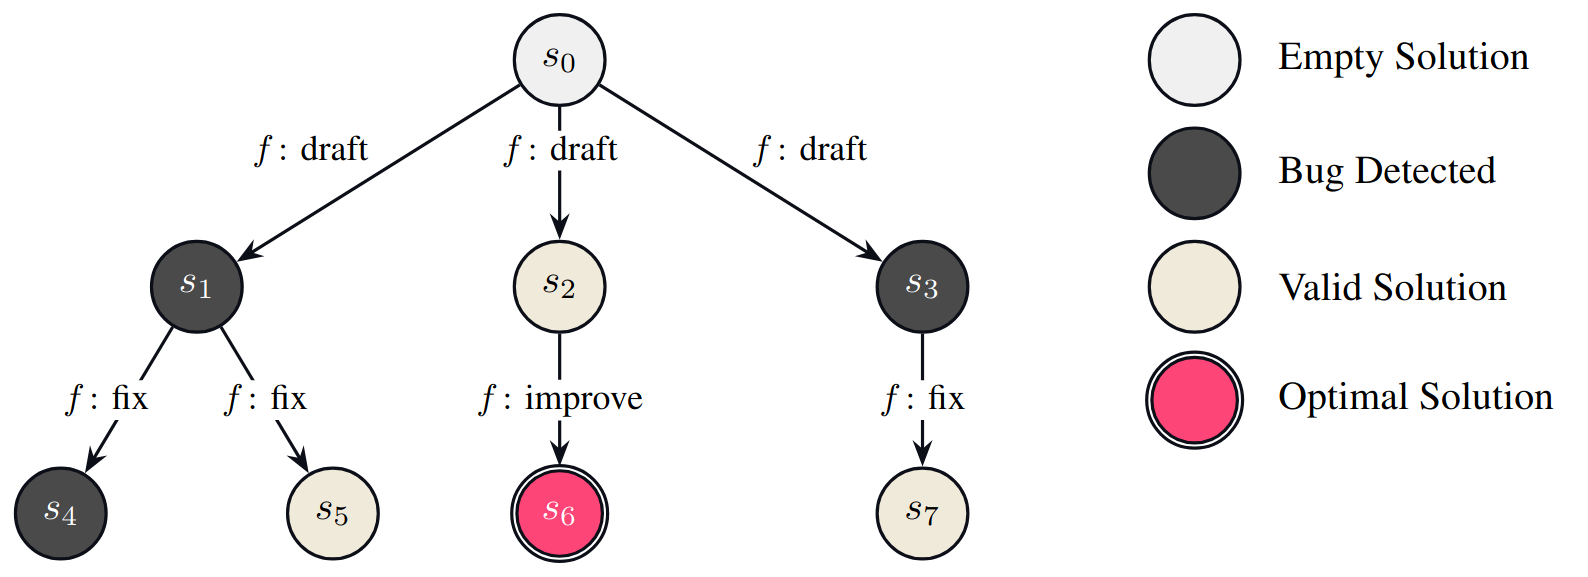
\includegraphics[width=0.8\linewidth]{images/aide-solution-tree.png}
%     \caption{A sample solution tree for AIDE, illustrating the drafting, fixing, and improvement steps. (Source: Schmidt et al., 2025, p. 4)}
%     \label{fig:enter-label}
% \end{figure}

% The Solution Tree ($T$): This is all discovered/proposed solutions (Python code scripts) and the improvement attempts (edges linking them) stored in a tree structure. The root solution ($s_0$) is typically an empty script, a node with value 'None'.

% Evaluator ($h$): This is a stateless function that takes a solution script as input and returns a scalar score (e.g., validation accuracy, loss). This score guides the search process. this evaluator is composed of a code interpreter that executes the code, then another LLM then takes the execution result (the trace back) and produces a structured output via function calling. this particular role is considered stateless since it always produce the same score, and it does not include past attempts in its evaluation, and this is important in the overall tree search for the best solution as every node or possible solution is evaluated primary on this.

% Search Policy ($\pi$): AIDE uses a simple, hard-coded search policy that determines the next step or next action. Based on the current state of the solution tree, it decides to:

% 1. Draft a new initial solution (if a desired number of diverse starting points hasn't been reached).

% 2. Debug a buggy node (if it's within a certain debug depth).

% 3. Improve an existing, non-buggy solution (typically targeting the current best-performing one).

% This policy has practical heuristics, such as initially exploring diverse solutions and then iteratively refining the most promising ones, while also limiting attempts to fix persistently broken solutions. Although this might be the most obvious area of improvement in the AIDE pipline, weather that was using a learned model that guides this search, the nature of the problems that small open source models have is largely not caused by the search heuristic, rather it is more fundamental in terms of ability to generate valid code in the first place, or correct usage of libraries and APIs.

% Coding Operator ($F$): This is the LLM itself as it proposes new scripts. It has three main entry points, each with specialized prompts:

% Drafting: Create a completely new solution `exploration`. The LLM is prompted to outline a plan to solve the problem (e.g., specify a neural network architecture and feature engineering ideas) and then generate a single-file Python program implementing that plan. These are then separated using regular expressions.

% Debugging: Repairing buggy solutions by inspecting error logs and execution traces. It attempts to fix issues like broken imports or incorrect tensor dimensions while preserving the overall approach.

% Improving: Called when a valid, non-buggy solution exists but could benefit from modifications (data preprocessing changes, architectural adjustments, or optimization tweaks and hiperparameter tuning). The LLM is prompted to propose a single `atomic` change, such as switching an optimizer or adding a regularization technique, so its impact on performance can be directly measured.

% Finally, to manage the LLM's context window and avoid `prompt explosion' from an  the growing history being fed to the model during the debugging and improvement phases, AIDE uses a summarization operator. Instead of appending all historical logs, this operator selectively extracts relevant information from the solution tree, such as Performance metrics (accuracy, AUC-ROC, etc.), Hyperparameter settings from previous attempts, Relevant hints for debugging (e.g., misaligned array shapes from trace-backs), This concise summary allows each code revision to be somewhat stateless yet guided by prior information, maintaining efficiency.

% Data Preview in Coding Prompts: AIDE also includes a small, static `data preview' in its coding prompts, providing the LLM with basic knowledge of the dataset's size or feature layout without needing extensive exploratory data analysis (EDA) at each step. As there is a code interpreter part of this iterative process, this Data preview tells the model exactly where and how the data is organized, and where to save its output or `submission.csv`

% The choice of AIDE as the foundational scaffold for this research is deliberate. It is open-source , it allows for the modification and integration of the inference-time scaling methods (self-consistency and self-reflection, etc) that are central to our work. Furthermore, AIDE's design, which explicitly models ML engineering as an iterative code optimization and tree search process powered by an LLM, provides a structured environment to study the effects of these techniques. It is established and proven to work effectively in solving ML tasks, as demonstrated in its original paper and subsequent evaluations on benchmarks like MLE-Bench, offers a great platform for experimentation. 

% AIDE has been tested and evaluated only using lagre-scale propriety LLMs, and our aim is to investigate how inference-time strategies can enhance AIDE's problem-solving capabilities, particularly its ability to make an open source, small-scale LLM generate more robust and higher-performing solutions on the challenging task like Machine learning Engineering.


% \section{MLE-Bench}
% To assess the performance of the enhanced aide scaffold we developed, we utilize the newly released MLE-bench, a benchmark for measuring how well AI agents perform at machine learning engineering, it is composed of 75 kaggle competitions, curated carefully from the Metakaggle dataset that contains around 5000 Kaggle competitions.
% This benchmark is designed specifically to be a benchmark for evaluating the performance of AI agents at machine learning engineering. MLE-Bench vary in category, scale, and complexity. This benchmark is designed not merely to test isolated skills, but to measure an agent's capacity for autonomous, end-to-end problem-solving—a workflow that spans model creation, training, evaluation, and iterative refinement.

% While MLE-Bench is a recent development, it is built upon a foundation of prior work aimed at evaluating LLMs coding and agentic abilities. Benchmarks like APPS (Hendrycks et al., 2021) and early evaluations of models such as Codex (Chen et al., 2021) have been used to measure general coding competence. The choice of MLE-Bench, and its particular relevance to this thesis, lies in its focus on tasks that are both representative of modern industry practices and known to be challenging for current AI systems, it offers a more specialized and demanding evaluation. However, it is very big benchmark, and evaluating on the 75 competitions is computationally infeasable for this thesis, hece, we opted for a subset of the benchmark,
% The core design of MLE-Bench is mostly around its task selection. The 75 selected competitions present an extremly difficult challenge for any coding agent. Essentially, MLE-Bench provides an offline Kaggle competition environment. For context, Kaggle is a platform that hosts data science and ML competitions where participants build predictive models to solve real-world challenges, competing for the best score on predefined metrics and earning rankings on a leaderboard. Top performers are often awarded monetary prizes, in addition to recognition with a bronze, silver, or gold medals. MLE-Bench adopts a similar structure to Kaggle, allowing for a realistic comparison of agent performance against historical human achievements 'offline leaderboard. The final results in this benchmark are often presented in terms of the average number of medals an agent would have won, determined by comparing its solution's metric on an unseen test set against the saved leaderboard from the original Kaggle competition.



% \section{Experiment Setup}

% To provide a rigorous and reliable evaluation of the inference-time strategies proposed in this thesis, a carefully designed experimental setup is essential. This section outlines the benchmark competitions, the baselines for comparison, the specific metrics used for evaluation, and the overall experimental procedure. The primary goal is to establish a solid evaluation framework that can take a given agent configuration as input and produce clear, quantitative metrics to determine its effectiveness relative to other methods.

% 1. Benchmark Competitions

% The foundation of our evaluation is a representative subset of competitions from the official MLE-Bench framework. While the full MLE-Bench is extensive, running experiments on all 75 competitions is computationally prohibitive for this project. Therefore, I have selected a curated subset of 10 competitions from the 'lite' complexity category. This choice was driven by several factors:

% Diversity: The selected competitions span 6 distinct machine learning categories, ensuring that our evaluation is not biased towards a single problem type. This diversity is crucial for assessing the general applicability of the proposed inference strategies.

% Feasibility: By focusing on 'lite' competitions, which are relatively lightweight in terms of data size and complexity, our experiments can focus on the quality of the agent's problem-solving process rather than being constrained by the technical overhead of handling massive datasets.

% Representativeness: This subset is a good representation of the full 'lite' category and provides a strong, empirical basis for evaluation.

% Flexibility: The chosen set is flexible enough to be extended in future work, either by including more competitions from the 'lite' category for a full standard comparison or by adding selected 'medium' complexity tasks to further test the limits of our methods.

% The 10 competitions selected for this benchmark are detailed in Table \ref{tab:competitions}.

% % \begin{table}[h!]
% % \centering
% % \caption{Selected Benchmark Competitions from MLE-Bench 'Lite' Category}
% % \label{tab:competitions}
% % \begin{tabular}{ll}
% % \hline
% % \textbf{Competition Name} & \textbf{Category} \ \hline
% % aerial-cactus-identification & Image Classification \
% % leaf-classification & Image Classification \
% % spooky-author-identification & Text Classification \
% % random-acts-of-pizza & Text Classification \
% % tabular-playground-series-may-2022 & Tabular \
% % nomad2018-predict-transparent-conductors & Tabular \
% % denoising-dirty-documents & Image to Image \
% % text-normalization-challenge-english-language & Sequence to Sequence \
% % text-normalization-challenge-russian-language & Sequence to Sequence \
% % mlsp-2013-birds & Audio Classification \ \hline
% % \end{tabular}
% % \end{table}

% 2. Baselines for Comparison

% To properly contextualize the performance of our proposed methods, we will benchmark them against a diverse set of established baselines. The aim is twofold: first, to prove that our strategies provide a meaningful improvement over a standard open-source model, and second, to demonstrate that these strategies make open-source models competitive with both closed-source counterparts and human experts.

% The baselines are summarized in Table \ref{tab:baselines}.

% % \begin{table}[h!]
% % \centering
% % \caption{Baselines for Performance Comparison}
% % \label{tab:baselines}
% % \begin{tabular}{lll}
% % \hline
% % \textbf{Baseline} & \textbf{Type} & \textbf{Reason for Inclusion} \ \hline
% % \textbf{AIDE + GPT-4o} & CS / High-Capability & Represents a strong, widely-used frontier model. \
% % & & Provides a high-water mark for performance. \ \
% % \textbf{AIDE + o4-mini} & CS / Reasoning-Optimized & Assumed to be a cost-effective, state-of-the-art reasoning \
% % & & model from OpenAI. Serves as a key SOTA reference. \ \
% % \textbf{AIDE + Llama 3.1 (405B)} & OS / High-Capability & A top-tier open-source model. Outperforming this \
% % & & demonstrates the power of our strategy. \ \
% % \textbf{Our Model + Default AIDE} & OS / Ablation & \textbf{Critical baseline.} This isolates the performance gain \
% % & & attributable specifically to our inference strategies, \
% % & & by removing them from our chosen model. \ \
% % \textbf{Human Performance} & Human Eval & Provides real-world context by comparing agent scores \
% % & & to the original Kaggle leaderboards. \ \hline
% % \end{tabular}
% % \end{table}

% 3. Evaluation Metrics

% To capture a holistic view of agent performance, we will use a suite of metrics inspired directly by the MLE-Bench and AIDE papers. These metrics evaluate an agent's ability to produce functional code, understand the task requirements, and ultimately generate an optimal solution.

% Code and Submission Generation: These metrics assess the fundamental ability of the agent to generate working code and complete the task.

% Valid Code Rate (\%): The number of steps that produce a valid, executable script divided by the total number of steps, averaged across seeds and competitions. A higher rate indicates a stronger fundamental code generation capability.

% Valid Submission Rate (\%): The percentage of independent runs (i.e., per seed, per competition) that successfully produce a submission file that passes the benchmark's validity checks. This is a stricter measure of task completion.

% Performance Against Human Baselines: Once a valid submission is produced, its quality is scored against the historical human leaderboard.

% Above Median (\%): The percentage of competitions where the agent's best score is strictly better than the median score achieved by human participants.

% Any Medal (\%): The percentage of competitions where the agent's best score is high enough to have earned a bronze, silver, or gold medal according to official Kaggle rules. This is our headline metric for overall success.

% The final results for each agent configuration will be presented in a summary table, as shown in the template in Table \ref{tab:results_template}.

% % \begin{table}[h!]
% % \centering
% % \caption{Template for Aggregated Results Table}
% % \label{tab:results_template}
% % \begin{tabular}{lccc}
% % \hline
% % \textbf{Model + Method} & \textbf{Valid Submission (\%)} & \textbf{Above Median (\%)} & \textbf{Any Medal (\%)} \ \hline
% % AIDE + o4-mini & X% 
% % ±
% % ±
% %  Y & X% 
% % ±
% % ±
% %  Y & X% 
% % ±
% % ±
% %  Y \
% % Our Model + Strategy 1 & X% 
% % ±
% % ±
% %  Y & X% 
% % ±
% % ±
% %  Y & X% 
% % ±
% % ±
% %  Y \
% % Our Model + Default AIDE & X% 
% % ±
% % ±
% %  Y & X% 
% % ±
% % ±
% %  Y & X% 
% % ±
% % ±
% %  Y \ \hline
% % \end{tabular}
% % \end{table}

% 4. Experimental Procedure

% To ensure a fair and repeatable evaluation, all experiments are conducted using a standardized protocol within a consistent environment.

% Environment: All runs are executed within a Dockerized environment to ensure consistency. AIDE is configured with fixed hyperparameters for all methods (e.g., 20 steps per attempt, 5 initial drafts).

% Execution: For each of the 10 competitions, every agent configuration ("Method") is run for k=3 independent attempts (seeds). This helps account for the inherent stochasticity of LLMs.

% Data Collection: After each run, we automatically collect the raw data, including whether a valid submission was generated and its corresponding score.

% Metric Calculation: Using the collected data, we calculate the flags for Valid Submission, Above Median, and Any Medal for each run.

% Aggregation: These flags are then aggregated. For metrics like Above Median and Any Medal, we consider a competition "solved" if at least one of the three seeds was successful (a pass@3 approach). The final percentages are averaged across the 10 competitions, with results reported as mean ± standard error.

% This standardized pipeline ensures that as we introduce and test new inference-time strategies, the results are directly and fairly comparable to our established baselines.



% % This is essentially what AIDE’s “solution tree” does conceptually – it navigates a solution space tree by proposing variations and seeing which yields better scores. Another formulation is the Tree-of-Thoughts
% % approach (Yao et al., 2023) where the model can propose multiple thoughts (steps of a solution)

% % This is somewhat what AIDE does by default (running the full training code to get a score), but one could go further and allow fine-grained tool use: the agent could execute just a part of the code (say a data pre-processing step) to inspect intermediate results, or call a library function to check documentation, etc. Another tool is a web browser or documentation fetcher, useful if the coding problem needs external knowledge
% % (though MLE-bench specifically disallows internet to prevent cheating). Still, 

% % For instance, in
% % OpenAI’s tests, they tried different “scaffolds”: AIDE, ResearchAgent, CodeAct, etc., each of which
% % structures the LLM’s process differently. 

% % AIDE’s self-reflection is essentially
% % an internal critic role given to the same model. We could also have a different model entirely
% % serve as the critic – for instance, use a 13B model to generate code and a more reliable 13B or
% % a set of heuristic rules to review it. This two-model system was not explicitly used in AIDE (to
% % our knowledge, AIDE uses one model for everything), but it’s a viable ITS approach: compose
% % multiple smaller experts rather than rely on one monolith. Each expert at inference time does
% % part of the task. 

% % search algorithms to explore solution space, tool use to gain information or verify outputs during generation, and modular agent frameworks that break the task into
% % pieces handled sequentially. These methods have proven effective: for example, using a Process Reward
% % Model + search enabled a 3B model to outperform a 70B model on a math benchmark, and
% % self-debugging allowed models to fix errors that they would otherwise miss. Importantly, most of these
% % techniques do not require fine-tuning the base model – they work by manipulating the inference
% % process (through prompting, iterating, or orchestration). Some advanced methods do introduce learned
% % components (e.g. training a verifier network, or fine-tuning the model to better utilize reflections), which blurs the line between pure inference-time and training. We’ll discuss a few such cases as well, but
% % the primary focus is on what can be done on the fly with an off-the-shelf model. The ultimate goal of
% % 5these strategies is well captured by OpenAI’s notion of “self-verification”, where the model can reliably
% % check its own work instead of relying on a giant ensemble or an external judge. In the next section,
% % we propose concrete techniques from these categories that AIDE could adopt to further empower its
% % small-model code generation in the ML domain.
% % **EITHER SPEAK ABOUT AIDE AND MLE BENCH HERE OR IN THE METHODS SECTINO** % You do not need to have exactly 4 chapters.
%                  % It is probably a good minimum, with 5 chapters 
%                  % average, and 7 chapters might be a maximum.
% % \chapter{Summary of Results}

% This chapter provides a concise overview of the experimental results, presenting the key aggregate performance metrics and empirical code generation capabilities for the evaluated agent configurations on the MLE-Bench subset.

% \section{Aggregate Performance Summary}

% Table \ref{tab:summary_aggregate} summarizes the overall performance of each model configuration, focusing on key metrics such as Valid Submission Rate (VSR), Above Median Rate (AMR), and Any Medal Rate (Pass@3). Made Submission is also included as a primary pipeline success indicator.

% \begin{table}[h!]
%     \centering
%     \caption{Summary of Aggregate Performance Metrics}
%     \label{tab:summary_aggregate}
%     % Using tabularx to make the table fit within the text width
%     \begin{tabularx}{\textwidth}{p{4.5cm} *{4}{>{\centering\arraybackslash}X}}
%         \toprule
%         Method                      & Made Submission (\%) & Valid Submission (\%) & Above Median (\%) & Any Medal (Pass@3 \%) \\
%         \midrule
%         \textbf{AIDE} & & & & \\
%         AIDE + o1-preview          & - & - & - & - \\
%         AIDE + GPT-4-turbo         & 73.3 $\pm$ 3.3 & 63.3 $\pm$ 3.3 & 20.0 $\pm$ 5.8 & 6.7 \\ % Pass@3 based on provided table
%         AIDE + gpt-4o-mini         & 76.7 $\pm$ 2.4 & 63.3 $\pm$ 2.4 & 26.7 $\pm$ 2.4 & 10.0 \\ % Pass@3 based on provided table
%         AIDE + DeepSeek-7B (Base)  & 23.3 $\pm$ 3.3 & 20.0 $\pm$ 0.0 & 0.0 $\pm$ 0.0 & 0.0 \\ % Pass@3 based on provided table
%         AIDE + DeepSeek-7B + SR    & - & - & - & - \\
%         AIDE + DeepSeek-14B (Base) & 73.3 $\pm$ 2.4 & 60.0 $\pm$ 4.1 & 10.0 $\pm$ 4.1 & 10.0 \\ % Pass@3 based on provided table
%         AIDE + DeepSeek-14B + SR   & - & - & - & - \\
%         AIDE + DeepSeek-32B (Base) & 76.7 $\pm$ 3.3 & 63.3 $\pm$ 3.3 & 33.3 $\pm$ 3.3 & 20.0 \\ % Pass@3 based on provided table
%         AIDE + DeepSeek-32B + SR   & - & - & - & - \\
%         \midrule
%         \textbf{Human Performance} & - & - & 50.0 & 12.4 \\
%         \bottomrule
%     \end{tabularx}
%     \caption*{\textbf{Note}: Metrics are mean $\pm$ standard error of the mean, averaged across 10 competitions and 3 seeds, except for Pass@3 which is the percentage of competitions with at least one medal across 3 seeds. SR denotes Self-Reflection strategy. Entries marked '-' indicate data was not available in the provided context.}
% \end{table}

% \section{Empirical Code Generation and Submission Attempt Summary}

% Table \ref{tab:summary_empirical} provides a summary of the average empirical metrics, highlighting the agent's code generation capabilities and pipeline progression based on Valid Code Generation Rate (VCGR), CSV Submission Attempt Rate (CSAR), Average Steps to First Working Output (StepsToWO), and Average Code Quality.

% \begin{table}[h!]
%     \centering
%     \caption{Summary of Empirical Code Generation and Submission Attempt Metrics}
%     \label{tab:summary_empirical}
%     % Using tabularx to make the table fit within the text width
%     \begin{tabularx}{\textwidth}{p{4.5cm} *{5}{>{\centering\arraybackslash}X}}
%         \toprule
%         Metric                     & AIDE + gpt-4o-mini & AIDE + GPT-4-turbo & AIDE + DeepSeek-7B (Base) & AIDE + DeepSeek-14B (Base) & AIDE + DeepSeek-32B (Base) \\
%         \midrule
%         VCGR (\%)                   & 40.53              & 40.40              & 3.73                      & 24.83                      & 25.63                      \\
%         CSAR (\%)                   & 41.47              & 41.87              & 4.93                      & 29.24                      & 26.50                      \\
%         Avg. Steps to First WO     & 9.77               & 12.00              & 28.77                     & 13.86                      & 13.56                      \\
%         Avg. Code Quality (1-10)    & 5.76               & 5.86               & 3.66                      & 5.00                       & 5.26                       \\
%         \bottomrule
%     \end{tabularx}
%     \caption*{\textbf{Note}: Metrics are averaged over all available runs (typically 10 competitions $\times$ 3 seeds). VCGR is the percentage of steps generating valid code. CSAR is the percentage of steps attempting a CSV submission. StepsToWO is the average number of steps to the first working output (using the \texttt{StepsToWO\_inf\_replaced} value from the source data). Avg. Code Quality is on a scale of 1--10. Data for models with the Self-Reflection strategy was not available in the provided aggregate empirical summaries.}
% \end{table} % Conclusion is usually a chapter itself. 
% %\chapter{Discussion and Conclusion}

This chapter provides a concise overview of the experimental results, presenting the key aggregate performance metrics and empirical code generation capabilities for the evaluated agent configurations on the MLE-Bench subset.

\section{Aggregate Performance Summary}

Table \ref{tab:summary_aggregate} summarizes the overall performance of each model configuration, focusing on key metrics such as Valid Submission Rate (VSR), Above Median Rate (AMR), and Any Medal Rate (Pass@3). Made Submission is also included as a primary pipeline success indicator.

\begin{table}[h!]
    \centering
    \caption{Summary of Aggregate Performance Metrics}
    \label{tab:summary_aggregate}
    % Using tabularx to make the table fit within the text width
    \begin{tabularx}{\textwidth}{p{4.5cm} *{4}{>{\centering\arraybackslash}X}}
        \toprule
        Method                      & Made Submission (\%) & Valid Submission (\%) & Above Median (\%) & Any Medal (Pass@3 \%) \\
        \midrule
        \textbf{AIDE} & & & & \\
        AIDE + o1-preview          & - & - & - & - \\
        AIDE + GPT-4-turbo         & 73.3 $\pm$ 3.3 & 63.3 $\pm$ 3.3 & 20.0 $\pm$ 5.8 & 6.7 \\ % Pass@3 based on provided table
        AIDE + gpt-4o-mini         & 76.7 $\pm$ 2.4 & 63.3 $\pm$ 2.4 & 26.7 $\pm$ 2.4 & 10.0 \\ % Pass@3 based on provided table
        AIDE + DeepSeek-7B (Base)  & 23.3 $\pm$ 3.3 & 20.0 $\pm$ 0.0 & 0.0 $\pm$ 0.0 & 0.0 \\ % Pass@3 based on provided table
        AIDE + DeepSeek-7B + SR    & - & - & - & - \\
        AIDE + DeepSeek-14B (Base) & 73.3 $\pm$ 2.4 & 60.0 $\pm$ 4.1 & 10.0 $\pm$ 4.1 & 10.0 \\ % Pass@3 based on provided table
        AIDE + DeepSeek-14B + SR   & - & - & - & - \\
        AIDE + DeepSeek-32B (Base) & 76.7 $\pm$ 3.3 & 63.3 $\pm$ 3.3 & 33.3 $\pm$ 3.3 & 20.0 \\ % Pass@3 based on provided table
        AIDE + DeepSeek-32B + SR   & - & - & - & - \\
        \midrule
        \textbf{Human Performance} & - & - & 50.0 & 12.4 \\
        \bottomrule
    \end{tabularx}
    \caption*{\textbf{Note}: Metrics are mean $\pm$ standard error of the mean, averaged across 10 competitions and 3 seeds, except for Pass@3 which is the percentage of competitions with at least one medal across 3 seeds. SR denotes Self-Reflection strategy. Entries marked '-' indicate data was not available in the provided context.}
\end{table}

% \section{Empirical Code Generation and Submission Attempt Summary}

% Table \ref{tab:summary_empirical} provides a summary of the average empirical metrics, highlighting the agent's code generation capabilities and pipeline progression based on Valid Code Generation Rate (VCGR), CSV Submission Attempt Rate (CSAR), Average Steps to First Working Output (StepsToWO), and Average Code Quality.

% \begin{table}[h!]
%     \centering
%     \caption{Summary of Empirical Code Generation and Submission Attempt Metrics}
%     \label{tab:summary_empirical}
%     % Using tabularx to make the table fit within the text width
%     \begin{tabularx}{\textwidth}{p{4.5cm} *{5}{>{\centering\arraybackslash}X}}
%         \toprule
%         Metric                     & AIDE + gpt-4o-mini & AIDE + GPT-4-turbo & AIDE + DeepSeek-7B (Base) & AIDE + DeepSeek-14B (Base) & AIDE + DeepSeek-32B (Base) \\
%         \midrule
%         VCGR (\%)                   & 40.53              & 40.40              & 3.73                      & 24.83                      & 25.63                      \\
%         CSAR (\%)                   & 41.47              & 41.87              & 4.93                      & 29.24                      & 26.50                      \\
%         Avg. Steps to First WO     & 9.77               & 12.00              & 28.77                     & 13.86                      & 13.56                      \\
%         Avg. Code Quality (1-10)    & 5.76               & 5.86               & 3.66                      & 5.00                       & 5.26                       \\
%         \bottomrule
%     \end{tabularx}
%     \caption*{\textbf{Note}: Metrics are averaged over all available runs (typically 10 competitions $\times$ 3 seeds). VCGR is the percentage of steps generating valid code. CSAR is the percentage of steps attempting a CSV submission. StepsToWO is the average number of steps to the first working output (using the \texttt{StepsToWO\_inf\_replaced} value from the source data). Avg. Code Quality is on a scale of 1--10. Data for models with the Self-Reflection strategy was not available in the provided aggregate empirical summaries.}
% \end{table} % You may have more chapters. (Use e.g. git add FILE)
% % This is where we stop counting pages.
% % Acknowledgements and References are not counted.
% %-----------------------------------------------------------------------------
% % See the acknowledgement.tex file and follow the instructions there.
% \chapter*{Acknowledgements}
% Don't change anything above this.
% We do not number this or add it to the contents!
% Overly long acknowledgements are not professional.

I want to acknowledge AIMS and it's funders for supporting this work, as well as my supervisor, Prof Arnu Pretorius from University of Stellenbosch, and my co-supervisor, Arnol Fokam from InstaDeep.

I would also like to thank my family and friends, and my colleagues at AIMS for their support and encouragement.

% %-----------------------------------------------------------------------------
% % Note the errata page is not for now, it is for use during the examination.
% % Not that you're going to have any errata.
% %-----------------------------------------------------------------------------
% % THE BIBLIOGRAPHY 
% % Bibliography styles define how the bibliography is 
% % listed and formatted. This is part of the AIMS house
% % style and is only changed under exceptional circumstances
% \renewcommand{\bibname}{References}
% \nocite{*}
% \bibliographystyle{myabbrvnat}
% \bibliography{references}
% \addcontentsline{toc}{chapter}{References}
% %-----------------------------------------------------------------------------
% \end{document}


% Explain the context of your research project topic, so that the
% topic itself appears motivated, natural and important.

% Paragraphs are separated by blank lines in the \LaTeX\ code, 
% and the line spacing, paragraph indentation,
% and paragraph spacing are set in the preamble for you, 
% according to AIMS house style.